\documentclass[conference]{IEEEtran}

% -------------------------
% Packages
% -------------------------
\usepackage{cite}
\usepackage{graphicx}
\usepackage{booktabs}
\usepackage{longtable}
\usepackage{hhline}
\usepackage[table]{xcolor}
\usepackage{amsmath,amsfonts}
\usepackage{bm}
\usepackage{multirow}
\usepackage{wrapfig}
\usepackage{comment}
\usepackage{import}
\usepackage[ruled,vlined,linesnumbered]{algorithm2e}
\usepackage{enumerate}
\usepackage{enumitem}
\usepackage{balance}
\usepackage[caption=false,font=footnotesize]{subfig}
\usepackage{xurl}
\usepackage{url}
\usepackage{float}

\usepackage[T1]{fontenc}
\usepackage[utf8]{inputenc}
\usepackage{tikz}
\usepackage{xcolor}
\newcommand{\cq}[1]{\textcolor{black}{#1}}

\usepackage{amsthm}

\newtheorem{lemma}{Lemma}
\newtheorem{definition}{Definition}
\newtheorem{theorem}{Theorem}

% \newcommand*\circled[2][black]{%
%   \tikz[baseline=(char.base)]{\node[
%     shape=circle, draw=none, thick,
%     fill=#1, inner sep=0.9pt] (char)
%   {\textcolor{white}{#2}};}}

\DeclareRobustCommand{\circled}[2][black]{%
  \tikz[baseline=(char.base)]{
    \node[
      circle,
      fill=#1,
      inner sep=0pt,
      minimum size=1.2em
    ] (char)
    {\scriptsize\textcolor{white}{#2}};
  }%
}

% -------------------------
% Your comment macros
% -------------------------
\newcommand{\yj}[1]{\textcolor{blue}{[\small YJ: ~#1~]}}
\newcommand{\YJ}[1]{\textcolor{red}{[\small YJ: ~#1~]}}
\newcommand{\CQ}[1]{\textcolor{brown}{[CQ: #1]}}

\AtBeginDocument{%
  \providecommand\BibTeX{{Bib\TeX}}}

\newcommand{\name}{\textsc{GIR}}

\begin{document}

\title{\name: A Persistent Intermediate Representation for Scalable Dynamic Graph Analytics}

% \title{\name: A Graph Intermediate Representation for Scalable Dynamic Graph Update and Computation}

% \author{
% \IEEEauthorblockN{Chaoqun Li, Yuede Ji}
% \IEEEauthorblockA{
% Department of Computer Science and Engineering\\
% The University of Texas at Arlington\\
% Arlington, Texas, USA
% }
% }

\maketitle

\begin{abstract}
% \begin{abstract}
% \YJ{TODO}
% Dynamic graphs demand both high-throughput structural updates and efficient, repeated
% downstream analytics. We present {\name}, a query-agnostic Graph Intermediate Representation
% that maintains multi-granular connectivity invariants—weakly connected components
% (WCC), strongly connected components (SCC) with a condensation DAG, and biconnected
% components (BiCC) organized as block-cut (BC) trees—and updates them incrementally
% using Scope–Prune–Update and Filter–Merge–Update strategies. By
% pruning at the DAG level and exposing independent BiCC blocks for concurrent
% execution, GIR enables block-level task parallelism that substantially reduces
% redundant downstream recomputation. We implement a GIR-enabled execution framework
% and evaluate it on seven real-world graphs (up to large scale), achieving up to
% 3.0× speedup on BFS, 2.7× on SSSP, and 1.7× on betweenness centrality while
% maintaining competitive update throughput and strong multi-thread scalability.
% \YJ{TODO}
% \end{abstract}
Dynamic graphs demand both high-throughput structural updates and efficient downstream analytics. 
Existing methods are either \textit{history-blind} as they discard prior computation after each update, incurring large repeated overhead
or \textit{query-dependent} as they reuse results but are tied to specific algorithms or parameters, offering no general
reuse. 
Neither approach captures algorithm-independent structural invariants as a persistent, reusable layer.
Inspired by compiler intermediate representations, we propose \textbf{GIR}, a
query-agnostic \emph{Graph Intermediate Representation} that decouples dynamic
graph updates from downstream query execution. GIR maintains a three-level
structural hierarchy of weakly connected components, strongly connected
components with a condensation DAG, and biconnected components
organized as block-cut trees. To keep GIR current under continuous updates,
we design strategies to confine each repair to the minimum affected region. GIR further enables a two-level parallel execution model that combines task parallelism across
independent blocks with data parallelism within each block. 
% Evaluated on
% seven real-world graphs, GIR achieves up to $3.0\times$ speedup on BFS,
% $2.7\times$ on SSSP, and $1.7\times$ on betweenness centrality over
% state-of-the-art systems, while maintaining competitive update throughput and
% near-linear scalability.
% We design {GIR}, a query-agnostic graph intermediate representation
% that bridges high-throughput dynamic graph updates and efficient downstream
% analytics. 
% GIR persistently maintains a three-level structural hierarchy of WCC, SCC, and BiCC, confines maintenance to the minimum affected region, and enables task parallelism.
% SCC with a condensation DAG, and BiCC with BC trees. 
% We confine maintenance to the minimum affected region, avoiding global recomputation.
% GIR further enables task parallelism.
Experiments on seven real-world graphs show that GIR achieves 1.8$\times$ more  update throughput than state-of-the-art methods.
For graph analytics, GIR achieves an average of 1.2$\times$, 1.2$\times$, and 1.7$\times$ speedups for breadth-first search, single-source shortest path, and betweenness centrality, respectively.
\end{abstract}

\section{Introduction}
\label{sec:introduction}

The graph is a fundamental abstraction for modeling relationships and 
dependencies across diverse domains, including social and information 
networks, transportation systems, cybersecurity provenance, and software 
package ecosystems~\cite{mislove2007measurement, leskovec2005graphs, 
kikas2017structure}. 
Among these, directed graphs 
% (digraphs)
are of particular interest 
as they capture asymmetric dependencies and causal flows that 
underpin critical analytics, such as breadth-first search (BFS)~\cite{lee1961algorithm}
%\YJ{add a citation for BFS, and later for SSSP and APSP} 
for traversal, single-source and all-pairs shortest paths (SSSP/APSP)~\cite{thorup1997undirected, seidel1992all}  for routing and dependency, and betweenness 
centrality (BC)~\cite{Brandes2001BC} for node importance.


Over the past years, graph processing systems and domain-specific 
frameworks have achieved substantial performance improvements for 
\emph{static} graph analytics on both CPUs and 
GPUs~\cite{Shun2013Ligra,Wang2016Gunrock,Zhang2018GraphIt}. 
% In parallel,  dynamic graph data structures have made it possible to ingest and  maintain evolving graphs under high update  rates~\cite{ediger2012stinger,Busato2018Hornet,Awad2020DynamicGPU}.
However, in many real-world domains, graphs are \emph{dynamic}, i.e., vertices and edges
continuously appear and disappear as the underlying system evolves~\cite{besta2021practice}. At the
same time, the users might issue \emph{ad hoc} queries with changing sources,
targets, and scopes. For example, a user may need to trace the blast
radius (i.e., the set of downstream services affected by a failure) of a newly
disclosed vulnerability, recompute reachability after
integrating new services, or update dependency analysis in an evolving
software ecosystem~\cite{brank2003download}. These traversal-centric tasks all
depend on the current graph structure and must be repeated as the graph evolves. These 
workloads combine continuous structural updates with repeated, query-driven 
traversals, forming an end-to-end pipeline that must be efficient in both 
dimensions.

Existing dynamic graph systems primarily focus on \textit{update throughput}, 
i.e., how quickly structural changes can be incorporated into the 
graph~\cite{ediger2012stinger,Busato2018Hornet,Awad2020DynamicGPU,fan2025cuckoograph}. 
However, update throughput only addresses part of the end-to-end workload. 
That is, after each structural change, downstream analytics such as BFS, SSSP, BC, 
and reachability often need to be recomputed, either partially or entirely. 
As graphs grow to billions of edges, such downstream graph analytics
% traversal-based algorithms 
increasingly dominate the total runtime. 
% In our experiments, downstream computation accounts for over $42.4\%$ \YJ{TODO\CQ{Done}}\CQ{42.4\% = downsteam time/ (downsteam time + building time)} of end-to-end execution time on large graphs~\cite{Hanauer2022DynSurvey}. 
Therefore, optimizing update throughput alone is not enough, while reducing the cost of downstream graph computation under 
continuous evolution is equally critical.

% Graphs provide a natural abstraction for modeling relationships and dependencies in domains such as social and information networks, transportation systems, cybersecurity provenance, and software package ecosystems~\cite{rahman2025hugginggraph, brank2003download,kikas2017structure}. 
% Directed graphs (digraphs) capture asymmetric dependencies and causal flows, which underpin fundamental analytics including breadth-first search (BFS), single-source and all-pairs shortest paths (SSSP/APSP), and betweenness centrality (BC)~\cite{Brandes2001BC}. 
% Over the past decade, graph processing systems and domain-specific frameworks have achieved substantial performance improvements for \emph{static} graph analytics on both CPUs and GPUs~\cite{Shun2013Ligra,Wang2016Gunrock,Zhang2018GraphIt}. 
% In parallel, dynamic graph data structures have made it possible to ingest and maintain evolving graphs under high update rates~\cite{Ediger2012Stinger,Busato2018Hornet,Awad2020DynamicGPU}.
% However, real-world graphs are not only \emph{large} but also inherently \emph{dynamic}. 
% Vertices and edges continuously appear and disappear, while analysts issue \emph{ad hoc} queries with changing sources, targets, and scopes. 
% For example, analysts may need to trace the blast radius of a newly disclosed vulnerability, recompute reachability after integrating new services, or update dependency analysis in evolving software ecosystems. %cite here

% Existing dynamic graph systems primarily focus on \textit{update throughput}, i.e., how quickly structural changes can be incorporated into the graph~\cite{Ediger2012Stinger,Busato2018Hornet,Awad2020DynamicGPU}. 



% While high update throughput is essential, it addresses only part of the end-to-end workload. 
% After each structural change, downstream analytics, such as BFS, SSSP, BC, and reachability, often need to be recomputed either partially or entirely. 
% As a result, in practical deployments, dynamic updates and downstream graph algorithms together form the end-to-end processing pipeline and frequently become the dominant computational bottleneck~\cite{Hanauer2022DynSurvey}. 
% In other words, optimizing updates alone is insufficient; the efficiency of downstream graph computation under continuous evolution is equally critical.

% \subsection{Motivation}
% \subsection{Two Extremes of Reusing Prior Computation}


% \begin{figure}[t]
%     \centering
%     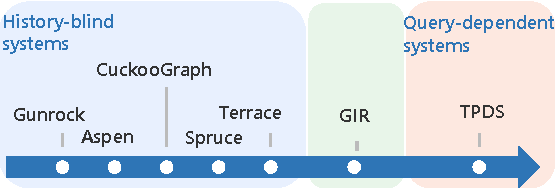
\includegraphics[width=\linewidth]{figures/history_blind-crop.pdf}
%     \caption{Dynamic graph systems classified by their use of prior
%     computation for downstream analytics.
%     History-blind systems (left) discard all prior results after each
%     update.
%     Query-dependent systems (right) cache results for a specific
%     query and source.
%     GIR (center) maintains query-agnostic structural invariants that
%     benefit all downstream algorithms.\YJ{Polish figure and caption to match this description. \CQ{Done}}}
%     \label{fig:history_query}
% \end{figure}

\textbf{Two extremes of reusing prior computation.} After a graph update, the results from previous computation do not 
simply become invalid.
Consider running SSSP from source $s$ on graph snapshot $G$,
when $G$ is updated to $G'$, many of the shortest paths from $s$ 
remain unchanged.
A system that could identify which results are still valid and which 
need to be recomputed would avoid a large fraction of redundant work.
However, the key question is, in what form should prior computation be retained to maximize reuse?
% As illustrated in Fig.~\ref{fig:history_query}, 
% Unfortunately, 
Existing approaches fall into two extremes, where they either igore such previous computation information (history-blind system) or overly rely on them (query-dependent system). 
% is well suited for ad hoc dynamic graph workloads.
% Particulalry,

\textit{(i) History-blind systems.}
Most dynamic graph systems, including Terrace~\cite{pandey2021terrace}, 
Spruce~\cite{shi2024spruce}, and Aspen~\cite{dhulipala2019low}, treat each query independently.
That is, after an update, such a system integrates the change into the graph representation and reruns the queried graph algorithm.
These systems are generic to any queries, while they discard the 
prior computation after every update.
For large graphs with frequent updates, such a system will incur large overhead due to repeated recomputation.
% is the dominant source of overhead.
% ~\cite{ramalingam1996computational}.

\textit{(ii) Query-dependent systems.}
A different class of systems try to reuse prior results more
directly.
For example,
% \textit{Khanda et al.}~\cite{khanda2021parallel} maintain an SSSP tree rooted at a fixed source $s$ after each query~\cite{khanda2021parallel}.
\textit{Khanda et al.} designed a method by maintaining  
% TPDS\cite{khanda2021parallel} maintains 
an SSSP tree rooted 
at a fixed source $s$~\cite{khanda2021parallel}.
\cq{Upon an update, they recompute only the affected subtree.
\textit{GraphBolt}~\cite{mariappan2019graphbolt} and
\textit{DZiG}~\cite{mariappan2021dzig} maintain per-vertex aggregation
dependencies for a fixed algorithm (e.g., PageRank) and propagate only the
incremental delta caused by mutations.
\textit{Kickstarter}~\cite{vora2017kickstarter} retains approximate monotonic results for path-based algorithms and propagates corrections after updates.
These approaches can be efficient when the same algorithm is repeated on the same graph.
However, they are tied to specific queries, e.g., a specific source vertex for SSSP query.
% However, each system is tied to a specific algorithm and, in some cases, a specific source vertex.
If the next query uses a different source, or switches to a different algorithm,
the cached state provides no benefit and must be rebuilt.}
In practice, dynamic graph workloads are dominated by \emph{ad hoc} queries
with varying sources, targets, and algorithms~\cite{Hanauer2022DynSurvey}.
Thus, such query-dependent systems offer limited reuse in practice.



% One natural way to reduce downstream recomputation is to retain and
% exploit the \emph{history of structural changes}.
% When an edge is inserted or deleted, not all downstream algorithms are
% equally affected.
% Only those that depend on the connectivity region touched by the update
% need to be re-executed.
% If a system could identify which structural invariants changed and which
% did not, downstream algorithms could skip unaffected regions entirely,
% rather than recomputing from scratch after every update.


% Modern applications increasingly rely on dynamic graphs, where edges and vertices evolve continuously over time. 
% Beyond the current snapshot, the \emph{history of updates} is essential for temporal reasoning, incremental computation, 
% and maintaining structural properties. However, existing systems treat history as either transient streams or low-level 
% storage artifacts, rather than a first-class abstraction for structural computation.



% As illustrated in Fig.~\ref{fig:history_query}, prior systems utilize history at different levels. 
% Streaming systems such as Terrace and Spruce process updates in an ephemeral manner, without retaining history for 
% structural reasoning. In contrast, systems like Aspen support versioned snapshots via persistent data structures, 
% enabling access to past states. However, such history remains at the data level and does not capture the evolution of 
% higher-level structures (e.g., SCCs or BCTs), leading to costly recomputation under updates.

% The key limitation is that \emph{history is stored but not understood}. Existing approaches fail to capture the semantic 
% impact of updates on graph structure, which is critical for connectivity-centric tasks.

% \textbf{A Compiler Mindset for Dynamic Graph}
% \subsection{A Compiler Mindset for Dynamic Graph}

\textbf{A compiler mindset for dynamic graph}.
The two extremes reveal a clear gap.
That is, we need a method that not only leverages historical computation results but also is not tied to any specific queries or algorithms.
% What is needed is a form of 
% prior computation that is incrementally maintained across updates and is not tied to any specific query or source.
% To address this gap, 
Inspired by the intermediate representation (IR) design in compiler~\cite{Lattner2004LLVM}, we propose a new  IR for dynamic graphs, named graph IR (GIR).
The goal is to capture \textbf{\textit{reusable structural invariants}} that persist across dynamic updates and can benefit many algorithms, without being tied to any specific queries or algorithms.

Just as a compiler IR sits between front-end parsing and back-end optimization passes, GIR sits between graph updates and downstream analytics.
% \YJ{working on}
As shown in Figure~\ref{fig:gir_ir}, this mirrors the compiler
pipeline. That is, updates modify the graph structure (analogous to front-end), 
and downstream algorithms repeatedly operate on the result
(analogous to optimizations).


% To address this, we propose a \emph{Graph Intermediate Representation (GIR)} that elevates history to a 
% \emph{structure-aware abstraction}. GIR maintains a compressed history that encodes structural evolution, enabling 
% efficient incremental updates across multi-granular connectivity representations. Instead of recomputing from scratch 
% or replaying full histories, GIR localizes changes and propagates updates efficiently across hierarchical structures.

% \YJ{Need more discussions on dynamic graph algorithm computation.}

% \textbf{Dynamic graph algorithm computation in practice.}
% Although theoretical research has proposed sophisticated fully dynamic algorithms for reachability, connectivity, and shortest paths~\cite{King1999TransitiveClosure,Demetrescu2004DynamicAPSP}, as well as incremental techniques for SSSP and centrality~\cite{Ramalingam1996Incremental,Nasre2014IncBC}, bridging theory and practical systems remains challenging.
% First, many dynamic algorithms assume fixed sources or specific query patterns, whereas real workloads are dominated by \emph{ad hoc} queries with changing sources and scopes~\cite{Hanauer2022DynSurvey}.
% Second, deletions and structural churn may trigger complex dependency updates, leading to high worst-case repair costs.
% %Third, modern parallel hardware such as GPUs favors regular, bulk-synchronous execution, while dynamic maintenance often introduces irregular control flow and scattered memory accesses~\cite{Gao2024DynGPUSurvey}.
% We also observe that as graph size grows, downstream computation increasingly dominates overall runtime.
% For smaller graphs, update processing and downstream analytics contribute comparable costs.
% However, for larger graphs, traversal-based algorithms such as BFS, SSSP, and BC account for the majority of execution time.
% This observation suggests that optimizing update throughput alone is insufficient for improving the performance of dynamic graph systems.
% Consequently, even when update throughput is high, downstream graph algorithms still incur substantial recomputation overhead under continuous evolution.
% Instead, reducing the cost of downstream analytics is critical for achieving scalable end-to-end performance.


%\YJ{Need two types of numbers (better to be in a figure), 1. +how slow are the downstream graph algorithms. 2. how slow are the end-to-end computation.}

% \textbf{A compiler mindset for dynamic graphs.}
% In compiler design, an intermediate representation (IR) separates front-end parsing from back-end optimization, enabling multiple optimization passes without repeatedly analyzing the original source code~\cite{Lattner2004LLVM}. 
% We observe a similar separation in dynamic graph processing: dynamic updates continuously modify the graph structure (analogous to parsing), while downstream algorithms repeatedly operate on the evolving graph (analogous to optimization passes).
% Motivated by this perspective, we introduce the \textbf{Graph Intermediate Representation (GIR)}, a dynamic and query-agnostic representation that persists across updates and exposes reusable structural invariants for downstream analytics.
% \YJ{Add a figure to show the connection between IR and GIR.}


% GIR is guided by three design principles. 
% (i) First, the invariants must be \textit{algorithm-independent}, capturing structural properties that benefit many graph algorithms rather than any single one. 
% (ii) Second, they must be \textit{incrementally maintainable}, allowing each invariant to be repaired after a local graph update without full recomputation. 
% (iii) Third, they must be \textit{multi-granular}, collectively exposing graph structure at multiple levels, from global connectivity down to local articulation boundaries. so that algorithms can prune their search space at whichever level is most appropriate.

% GIR is guided by three design principles.
% (i) First, the invariants must be \emph{algorithm-independent}: they should capture structural properties
% that benefit many graph algorithms, not just one.
% (ii) Second, they must be \emph{incrementally maintainable}: each invariant should be repairable
% after a local graph update without a full recomputation.
% (iii) Third, they must be \emph{multi-granular}: together, they should expose graph structure
% at multiple levels, from global connectivity down to local articulation boundaries,
% so that algorithms can prune their search space at whichever level is appropriate.

% However, this GIR needs to be efficient for under dynamic workloads, which poses three key
% challenges.
% \textbf{(i)} \textit{High update velocity} requires low-latency structural
% repair after each edge insertion or
% deletion.
% \textbf{(ii)} It can handle \textit{ad hoc queries} that the query source and type
% change frequently.
% \textbf{(iii)} \textit{scale and skew}, where billion-edge graphs with
% heavy-tailed degree distributions stress memory locality and load
% balancing on multi-core and GPU
% systems.
% To address these challenges, GIR enforces strict scope control.
% Each update triggers only the minimal structural repairs necessary,
% preventing maintenance overhead from outweighing the gains in
% downstream performance.

%\begin{figure}[t] % \centering % 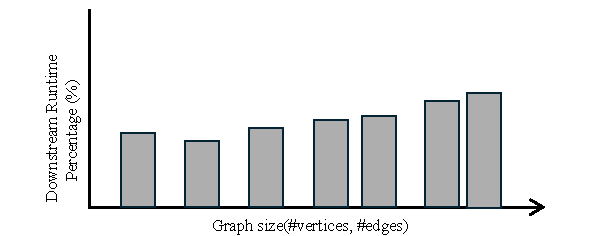
\includegraphics[width=\linewidth]{figures/Presentation2.pdf} %\caption{ %\textbf{Downstream computation increasingly dominates end-to-end runtime as graph size grows.} %The figure shows the percentage of runtime spent in downstream graph algorithms (e.g., BFS, SSSP, BC) relative to the total end-to-end processing time. %As the graph size increases, downstream computation becomes the dominant cost in the dynamic graph processing pipeline. %This trend highlights the importance of optimizing downstream analytics rather than focusing solely on update throughput. %\YJ{TODO} %} % \Description{Figure description.} % \label{fig:downstream_ratio} %\end{figure} %Figure~\ref{fig:downstream_ratio} illustrates how the runtime distribution changes as graph size increases. %The figure reports the percentage of runtime spent in downstream graph algorithms relative to the total end-to-end processing time.



% \YJ{This can merge with the previous paragraph. No need to discuss our concrete design of GIR at this stage.}

% Rather than caching answers for specific sources or queries, GIR maintains multi-granular connectivity structures—such as connected components (CC), strongly connected components (SCC) and their condensation DAG, and biconnected components (BiCC)—because these invariants provide algorithm-independent \emph{boundaries} and \emph{jump points}.
% These structural boundaries localize the impact of updates and allow traversal-based analytics to skip unaffected regions or shortcut exploration across certified structural cuts.
% \YJ{@YJ, needs further polishing.} \YJ{Challenges:
% Challenge 1. Inefficient graph update --> GIR;
% Challenge 2. Limited parallelism --> Concurrent computation framework} 

% Maintaining such structural information is challenging under three key properties of modern workloads:
% (i) \textbf{High update velocity}, which requires low-latency maintenance~\cite{Ediger2012Stinger,Busato2018Hornet};
% (ii) \textbf{Ad hoc queries}, which limit the effectiveness of source-specific caching~\cite{Hanauer2022DynSurvey};
% and (iii) \textbf{Scale and skew}, where billion-edge graphs with heavy-tailed degree distributions stress memory locality and load balancing on both CPUs and GPUs~\cite{Shun2013Ligra,Wang2016Gunrock,Zhang2018GraphIt,Gao2024DynGPUSurvey}.
% To prevent maintenance overhead from overwhelming query gains, our GIR also enforce strict \emph{scope control}, ensuring that each update triggers only the minimal necessary repairs.

% \subsection{Contribution}
% \label{subsec:contribution}

\begin{figure}[t]
    \centering
     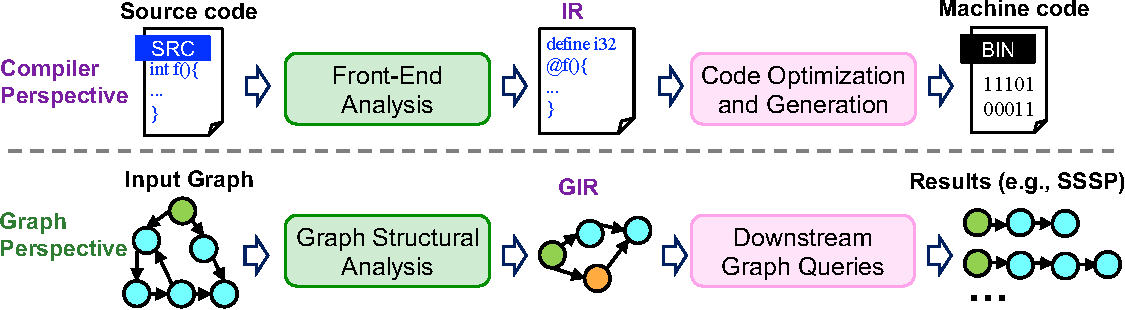
\includegraphics[width=1\linewidth]{figures/compiler_figure.pdf}
    \caption{\textit{From compiler IR to Graph IR (GIR).}
    Compiler IR enables reusable optimizations across different programming languages. Similarly, GIR maintains reusable structural invariants across dynamic updates.}
    \label{fig:gir_ir}
\end{figure}

% Particularly, this paper makes three major contributions.

\textbf{Contribution}.
Building GIR under continuous, high-velocity updates with ad hoc query patterns is nontrivial.
There are three challenges must be addressed.
\emph{(i) Update velocity}: low-latency GIR repair is required after each node/edge insertion or deletion.
\emph{(ii) Ad hoc queries}: the query source, target, and algorithm can change between requests. Thus, no query-specific state can be assumed.
\emph{(iii) Large scale graphs}: the graph could become large, e.g., with billion edges. Thus, the end-to-end computaiton, including update and query, needs to be efficient.
% sheer size of billion-edge graphs places sustained pressure on memory locality and makes efficient load balancing increasingly difficult on multi-core systems.
% \emph{(iii) Scale and skew}: billion-edge graphs with heavy-tailed degree distributions stress memory locality and load balancing on multi-core systems.
To address such challenges, this paper presents GIR, a scalable dynamic graph analytics system based on a newly designed persistent intermediate representation. Particularly, we make four major contributions.

% \textbf{Graph intermediate representation (GIR).}
% We devise GIR, a dynamic and query-agnostic structural layer for dynamic graphs.
% Particularly, the GIR integrates three fundamental structural algorithms. 
% \YJ{Why designing in this way.}
% First, \emph{weakly connected components (WCCs)} partition the graph into independent regions, which allow  downstream algorithms immediately skip entire components that are unreachable from a query source, pruning the largest unnecessary work at the coarsest level.
% Then, \emph{strongly connected components (SCCs) and their condensation directed acyclic craph (DAG)} capture directed
% reachability and cycle structure within each WCC.
% The condensation DAG reduces directed traversal to a DAG walk, eliminating redundant exploration of cyclic subgraphs.
% \emph{Biconnected components (BiCCs) and their block-cut tree (BCT)} expose articulation
% boundaries within each SCC.
% The BCT reveals which subgraphs are structurally independent, allowing algorithms to
% process each block separately without crossing unnecessary cut vertices.
% These algorithms are chosen because they are algorithm-independent structural invariants. They expose natural boundaries and hierarchical structure that many algorithms implicitly rediscover during computation.

\textbf{Graph intermediate representation (GIR).}
We devise GIR, a dynamic, query-agnostic structural layer for graphs. GIR integrates three fundamental primitives. First, \emph{weakly connected components (WCCs)} partition the graph into independent regions, enabling algorithms to skip unreachable components and prune work at a coarse level. Second, \emph{strongly connected components (SCCs)} and their condensation directed acyclic graph (DAG) capture directed reachability, reducing traversal to a DAG and avoiding redundant exploration of cycles. Third, \emph{biconnected components (BiCCs)} and the block-cut tree expose articulation boundaries, allowing independent processing of subgraphs. 
% These primitives are algorithm-agnostic structural invariants that reveal natural boundaries and hierarchy often rediscovered during computation.
These three primitives are chosen because they are algorithm-independent structural invariants that expose natural hierarchical boundaries many algorithms implicitly rediscover during computation.

\textbf{Structure-aware incremental maintenance.} We design an incremental maintenance method that keeps GIR structurally consistent under dynamic graph updates without full recomputation. 
\textit{The core insight is that GIR's three-layer hierarchy enables a metadata-only classification of every edge insertion or deletion into one of five structurally distinct cases, each confining repair to the minimum necessary region.}
We formalize this as a scope-prune-update strategy for single-edge updates and extend it to a filter-merge-update strategy for batch updates. 
Together, they eliminate redundant operations, merge overlapping maintenance regions, and enable parallel execution.
% across independent regions. 
% Together, they eliminate redundant operations, merge overlapping maintenance regions, and enable parallel execution across independent regions. 
% Compared to recent methods on dynamic graph computation, 
Benefited from this, for the update with both insertions and deletions, on all the tested graphs, GIR achieves an average throuput of $25.4$ million edges per second (MEPS), which is $1.8\times$ more than state-of-the-art methods.
% achieves an average of $8.5\times$, $1.9\times$, and $1.8\times$ speedup for update throughput over recent methods, including Spruce, Terrace, and Aspen, respectively.
%citation here

% On seven real-world graphs, GIR achieves 
% $8.5\times$ over Spruce, $1.9\times$ over Terrace, and $1.8\times$ over Aspen.
% average mixed-update throughput speedups of $8.5\times$ over Spruce, $1.9\times$ over Terrace, and $1.8\times$ over Aspen.
% Evaluated on seven real-world graphs, GIR achieves average mixed-update throughput speedups of $8.5\times$ over Spruce, $1.9\times$ over Terrace, and $1.8\times$ over Aspen.
%\YJ{Any benefit numbers? Like, how much throughput improvement?}
% Together, SPU and FMU provide correctness and efficiency guarantees that no flat or single-layer index can match.

% \textbf{Cascading repair ...}
% To maintain GIR efficiently, we develop the \emph{Scope-Prune-Update} strategy.
% SPU first identifies which structural layers are affected by an update, then restricts
% repair to the smallest affected region, and finally performs localized structural fixes.
% For batch updates, we extend SPU into the \emph{Filter-Merge-Update} pipeline,
% which removes redundant operations, groups related updates by affected region, and
% processes them in parallel.
% To the best of our knowledge, GIR is the first dynamic, query-agnostic intermediate
% representation that maintains multi-granular connectivity structures for reuse
% across downstream graph algorithms.
% including 
% weakly connected components (WCCs), strongly connected components
% (SCCs) and biconnected components (BiCCs).
% These invariants are algorithm-independent.
% They expose natural structural boundaries that traversal-based
% algorithms implicitly rediscover on every query.
% By keeping these boundaries explicit and up to date, GIR allows
% downstream algorithms to skip unaffected regions and shortcut
% traversal across structural cuts.
% The same GIR can accelerate BFS, SSSP, betweenness centrality, and
% reachability queries, without any query-specific precomputation.
% % GIR maintains WCCs, SCCs and their condensation DAG, and BiCCs
% % organized as block-cut trees, incrementally under continuous updates.
% % These invariants are reused across diverse downstream analytics,
% % avoiding redundant recomputation.
% To maintain GIR efficiently, we develop the {Scope-Prune-Update
% (SPU)} strategy.
% SPU first identifies which structural layers are affected by an
% update, then restricts repair to the smallest affected region, and
% finally performs localized structural fixes.
% This ensures that each update triggers only the minimal necessary
% work.
% For batch updates, we extend SPU into the {Filter-Merge-Update
% (FMU)} pipeline, which removes redundant operations, groups related
% updates by affected region, and processes them in parallel.
% To the best of our knowledge, GIR is the first dynamic,
% query-agnostic intermediate representation that maintains
% multi-granular connectivity structures for reuse across downstream
% graph algorithms.

\textbf{GIR-enabled two-level parallel execution.}
Conventional dynamic graph systems rely primarily on data parallelism,
% ~\cite{ediger2012stinger,Busato2018Hornet,Awad2020DynamicGPU,fan2025cuckoograph}, 
i.e., all threads work
on the same task simultaneously.
GIR unlocks a second, complementary form of parallelism, i.e., task parallelism.
As GIR explicitly decomposes the graph into independent structural units, multiple
units can be processed as concurrent tasks, each without inter-task synchronization.
% Taking BFS and SSSP as examples, 
% For BFS and SSSP, 
Taking BFS as an example,
we can prune their search space using the condensation DAG and then execute one task per BiCC block in parallel.
% For DFS, which is traditionally sequential and difficult to parallelize on flat graphs\cite{malumbres2000efficient},
% BiCC blocks provide naturally independent subtasks, making DFS parallelizable for the first time in a practical setting.
%\YJ{64 or 128?}
% Particularly, with 64 threads, our method achieves average $1.9\times$ task-level speedup over conventional graph execution on large graphs, including livejournal, twitter and friendster, by running BFS. 
% Particularly, on the tested graphs, GIR achieves an average of $3\times$, $1.3\times$, and $1.3\times$ speedup for running BFS over Spruce, Terrace, and Aspen, respectively. 
With the additional task parallelism, 
% Benefited from this, 
on all the tested graphs, GIR achieves an average of $1.2\times$, $1.2\times$, and $1.7\times$ speedups over state-of-the-art methods for running BFS, SSSP, and betweenness centrality (BC), respectively.
% $1.3- 3\times$ average speedups for BFS over state-of-the-art methods.
% besides BFS, on SSSP acheives $2.7\times$ average speedups,
% BC acheieves $1.7\times$ everage speedups by comparing with state-of-the-art methods


% \YJ{TODO}


% \YJ{TODO}
%\YJ{Be specific. Which graphs? Which compared methods?}
%\YJ{Fill in concrete numbers.\CQ{Done}}




\textbf{End-to-end evaluation.}
%update throughput
We evaluate GIR on seven real-world graphs covering social networks,
citation graphs, and web graphs, with the largest one having $2.4$ billion edges.
\cq{We compare GIR against state-of-the-art dynamic graph computation methods, i.e., Terrace~\cite{pandey2021terrace}, Aspen~\cite{dhulipala2019low}, and Spruce~\cite{shi2024spruce} for update throughput and BFS/BC analytics, and additionally against GraphBolt~\cite{mariappan2019graphbolt} and DZiG~\cite{mariappan2021dzig} for BFS/SSSP analytics.}
For update throughput,
on average, GIR achieves $22.6$ MEPS for \textit{insertion-only update}, which is $9.1\times$, $3.4\times$, and $2.7\times$ more than Spruce, Aspen, and Terrace, respectively. 
For \textit{deletion-only update}, GIR achieves $8.5\times$, $4.4\times$, $3.4\times$ over Spruce, Aspen, and Terrace, respectively. 
\cq{For downstream graph analytics, GIR achieves average speedups of $1.6\times$ on BFS over Spruce, Terrace, Aspen, GraphBolt, and DZiG.
% (up to $3\times$ over Spruce on structured graphs); 
% For SSSP, GIR achieves $2.7\times$ over Spruce, $1.6\times$ over DZiG, and $1.2\times$ over GraphBolt; 
For SSSP, GIR achieves $2.7\times$, $1.6\times$, and $1.2\times$ over Spruce, DZiG, and GraphBolt, respectively.
For BC, GIR achieves $1.7\times$ over Terrace and Aspen.}
In addition, GIR shows strong and stable scalability across all tested datasets.
% In addition, GIR shows strong and stable scalability, achieving $20.9\times$ average speedup at 64 threads, ahead of Spruce ($17\times$).
% on average, GIR achieves $22.6$ MEPS for \textit{insertion-only} updates ($9.1\times$, $3.4\times$, and $2.7\times$ over Spruce, Aspen, and Terrace) and $8.5\times$, $4.4\times$, $3.4\times$ more for \textit{deletion-only} updates.
% $9.1\times$, $3.4\times$, and $2.7\times$ more than Spruce, Aspen, and Terrace, respectively.
% \cq{For downstream graph analytics, GIR achieves average speedups of $1.3\times$ on BFS over Spruce, Terrace, Aspen, GraphBolt, and DZiG (up to $3\times$ over Spruce on structured graphs); 
% $2.7\times$ on SSSP over Spruce, $1.6\times$ over DZiG, and $1.2\times$ over GraphBolt; and $1.7\times$ on betweenness centrality over Terrace and Aspen.}
% In addition, GIR shows strong and stable scalability, achieving $20.9\times$ average speedup at 64 threads, ahead of Spruce ($17\times$).



%We compared GIR with state-of-the-art dynamic graph computation methods, including Terrace~\cite{pandey2021terrace}, Aspen~\cite{dhulipala2019low}, and Spruce~\cite{shi2024spruce}.
%\YJ{Two aspects, (1) update throuput; (2) performance on graph algorithms.}
%Besides the mixed (insertion and deletion update), 
% Specifically,or \textit{insertion update},
%on average, GIR achieves $22.6$ MEPS for \textit{insertion-only update}, which is $9.1\times$, $3.4\times$, and $2.7\times$ more than Spruce, Aspen, and Terrace, respectively. 
%For \textit{deletion-only update}, GIR achieves $8.5\times$, $4.4\times$, $3.4\times$ more than Spruce, Aspen, and Terrace, respectively. 
%for insersion-only updates, we achieve average $5.0\times$,  speedup $9.1\times$ over Spruce, $3.4\times$ over Aspen, $2.7\times$ over Terrace,
%for deletion-only updates, we achieve $8.5\times$ over spruce, $4.4\times$ over Aspen, $3.4\times$ over Terrace
%our average throughput is 25.4 meps versus Aspen 14 meps, Terrace 13.6 meps Spruce 3 meps
% on mixed insertion/deletion workloads, GIR
% achieves average speedups of $8.5\times$ over Spruce, $1.9\times$ over
% Terrace, and $1.8\times$ over Aspen.
% (ii) For downstream \textit{graph analytics}, GIR achieves an average $3\times$ speedup on BFS over Spruce, $2.7\times$ on SSSP over Spruce, and $1.7\times$ on BC over both Terrace and Aspen.
% (iii) 
% \textit{Scalability}: 
%In addition, GIR shows strong scalability.
%\YJ{TODO}
%That is, with 64 threads, GIR achieves xx speedups 
%GIR scales to average $47\times$--$50\times$ speedup at 64 threads, %on large graphs (LJ and WT), 
% achieves $6.8/times$ speedup 
%consistently outperforming all baselines at every thread count.
%In addition, GIR shows strong and stable scalability across all tested datasets.
% On average GIR achieves $20.9\times$ speedup at 64 threads, ahead of Spruce ($17\times$).
% On graphs with many independent BiCC blocks (WT and LJ), GIR reaches $47.4\times$ and $45\times$ self-speedup at 64 threads, outperforming Spruce ($17.0\times$ and $45\times$) and Aspen ($43.6\times$ and $45\times$) on WT.
% On graphs with fewer blocks (WG and CP), GIR reaches $7.5\times$ and $11.0\times$ at 64 threads.
% On average across all datasets, GIR achieves $20.9\times$ speedup at 64 threads, ahead of Spruce ($17.0\times$).
% \YJ{TODO}


%\YJ{Also discuss scalability.}


% \YJ{Fill in numbers from experiment section.\CQ{Done}}

% \subsection{Contribution}

% \YJ{For each contribution, we need to add numbers.}

% % Here we summarize the key contributions of our GIR design.
% % \YJ{Then, briefly discuss the specific contributions. One per paragraph.}
% We make three major contributions.

% \textbf{Graph Intermediate Representation (GIR).}
% We introduce GIR, a reusable and query-agnostic graph representation that maintains structural invariants and lightweight summaries under continuous updates, enabling diverse ad hoc analytics to avoid redundant recomputation. GIR complements dynamic graph stores that prioritize update throughput~\cite{Ediger2012Stinger,Busato2018Hornet,Awad2020DynamicGPU} and static graph DSLs that optimize compute-only performance~\cite{Shun2013Ligra,Wang2016Gunrock,Zhang2018GraphIt}.
% Based on GIR, we further develop the SPU strategy, an incremental maintenance method that restricts structural repairs to a bounded region of influence in the condensation structure, thereby avoiding global recomputation.
% Rather than optimizing a single algorithm, GIR provides a reusable structural backbone that supports multiple analytics simultaneously, similar to how a compiler IR supports multiple optimization passes.
% Our goal is to enable a responsiveness-oriented dynamic graph processing pipeline in which both updates and downstream computation can execute efficiently.

% To the best of our knowledge, prior work has not introduced a dynamic, query-agnostic intermediate representation that maintains multi-granular connectivity structures for reuse across downstream algorithms.
% % This gap motivates the design of GIR.

% \textbf{GIR-Enabled Task Parallel Execution Framework.}
% We design traversal kernels for BFS, SSSP, BC and DFS that leverage GIR structural hints to prune unnecessary exploration and accelerate query execution.
% By exploiting the hierarchical structure exposed by GIR, the framework also enables effective parallelization.
% Even algorithms that are traditionally sequential, such as DFS, can benefit from the structural parallelism provided by our framework.
% \YJ{Add measurable benefit numbers. E.g., how much parallelism has been improved.}


% \textbf{End-to-end evaluation.}
% Through extensive experiments on real and synthetic dynamic workloads, we demonstrate substantial improvements in downstream latency and overall end-to-end responsiveness while maintaining competitive update throughput on modern multi-core systems.

% \YJ{Needs further polishing.}
\section{Background}
\label{sec:background}




% \YJ{Merge this with the related work sections. Please add citations accordingly.}

%This section reviews graph representations, connectivity structures, and dynamic graph systems, and positions our work with respect to existing approaches.

% ============================================================
% \subsection{Graph Representation}
% ============================================================

\textbf{Static graph representation.}
High-performance graph processing systems rely on compressed
sparse formats such as CSR (Compressed Sparse Row) and CSC
(Compressed Sparse Column)~\cite{wheatman2018packed}.
These formats store adjacency information in contiguous arrays.
% ,enabling cache-efficient sequential access during traversal.
They form the foundation of major graph processing frameworks,
including Ligra~\cite{Shun2013Ligra},
Gunrock~\cite{Wang2016Gunrock}, and GraphIt~\cite{Zhang2018GraphIt}.
However, CSR and CSC are not suitable for dynamic workloads as vertex/edge insertions/deletions require rebuilding contiguous arrays, introducing significant overhead.
% under frequent updates.

\textbf{Dynamic graph representation.}
\begin{maybecut}
To support evolving graphs, recent systems propose specialized
in-memory structures that balance update cost and query
efficiency.
Terrace~\cite{pandey2021terrace} targets skewed graphs and uses
a hierarchical adjacency representation that adapts its storage
to vertex degree, improving locality and update efficiency on
power-law graphs~\cite{barabasi1999emergence}.
Spruce~\cite{shi2024spruce} combines compact indexing with
update-friendly adjacency organization, integrating dynamic
buffers with CSR-like sorted blocks and a read-optimized
concurrency protocol.
Aspen~\cite{dhulipala2019low} represents graphs using
compressed purely functional trees and exposes immutable
snapshot views that support concurrent readers across updates.
% CUT CANDIDATE: same one-line descriptions of Terrace/Spruce/Aspen
% repeated almost verbatim in experiment.tex's Baseline paragraph;
% condensed in \texttt{fixed} below.
\end{maybecut}
\begin{fixed}
To support evolving graphs, recent systems propose specialized
in-memory structures that balance update cost and query efficiency,
including Terrace~\cite{pandey2021terrace}, Spruce~\cite{shi2024spruce},
and Aspen~\cite{dhulipala2019low}; Section~\ref{sec:experiment} describes
each in detail as an experimental baseline.
\end{fixed}

\textbf{Incremental graph computation.}
A complementary approach maintains algorithm-specific state to avoid full recomputation after updates.
GraphBolt~\cite{mariappan2019graphbolt} tracks per-vertex aggregation dependencies across bulk-synchronous parallel (BSP) iterations and re-propagates only the delta induced by each mutation, supporting algorithms including SSSP and BFS.
DZiG~\cite{mariappan2021dzig} extends GraphBolt with sparsity-aware processing that skips zero-contribution edges, further reducing propagation work on sparse updates.
Both systems rely on Ligra-style static computation for initial results and are tightly coupled to the algorithm being executed; switching the query or source vertex requires rebuilding their cached state.


\begin{figure}[t]
    \centering
    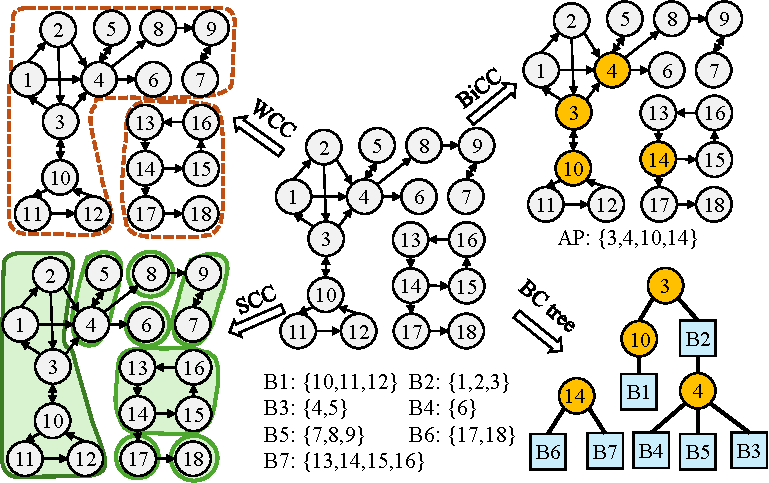
\includegraphics[width=\linewidth]{figures/scc_wcc_bcc-crop.pdf}
    \caption{Examples of weakly connected component (WCC), strongly connected component (SCC), biconnected component (BiCC), and block-cut (BC) tree.}
    \Description{An example directed graph annotated with its weakly connected components, strongly connected components, biconnected components, and the resulting block-cut tree.}
    % \YJ{TODO}}
    % \YJ{BC tree should look more like a "tree".\CQ{Done}}
    % }
    \label{fig:connectivity_example}
\end{figure}


% \YJ{Below discussions are too shallow. We need to touch the SOTA. Please rewrite.}
% \YJ{For static graphs, we should discuss adjacency matrix, adjacency list, and then emphasize CSR/CSC.}
% \YJ{For dynamic graphs, we need to clearly discuss the related works we have studied, such as, Terrace, Aspen, etc.}

% \textbf{Static graph representations.}
% Graph systems traditionally rely on several canonical representations.
% The earliest representations include adjacency matrices and adjacency lists.
% An adjacency matrix supports constant-time edge-existence queries but requires $O(n^2)$ memory, which makes it impractical for large sparse graphs.
% Adjacency lists significantly reduce memory usage to $O(n+m)$ and therefore form the basis of most traversal-based algorithms.

% Modern high-performance graph processing frameworks further adopt compressed sparse formats such as CSR (Compressed Sparse Row) and CSC (Compressed Sparse Column) ~\cite{wheatman2018packed}.
% These representations store adjacency information in contiguous arrays, enabling efficient sequential memory access and improved cache locality during neighborhood traversal.
% Consequently, CSR/CSC serve as the foundation of many static graph-processing systems, including Ligra~\cite{Shun2013Ligra}, Gunrock~\cite{Wang2016Gunrock}, and GraphIt~\cite{Zhang2018GraphIt}.

% Beyond classical CSR-based formats, some systems introduce alternative representations that support large-scale parallel graph analytics.
% For example, Aspen~\cite{dhulipala2019low} represents graphs using compressed purely-functional trees and exposes immutable \emph{snapshot} views for graph analytics.
% Each update produces a new graph version, enabling concurrent readers to operate on consistent snapshots while preserving structural sharing across versions.
% Although Aspen supports dynamic updates through versioning, its design primarily targets efficient analytics on static snapshots rather than fine-grained maintenance of continuously evolving graphs.

% Despite their efficiency for static workloads, CSR-based or snapshot-based representations are not well suited for highly dynamic environments.
% Edge insertions and deletions often require rebuilding large contiguous arrays or generating new graph versions, which introduces significant overhead when updates occur frequently.

% \textbf{Dynamic graph storage.}
% To support evolving graphs with interleaved updates and queries, recent systems propose specialized in-memory data structures that balance update cost, query efficiency, and memory usage.

% Terrace~\cite{pandey2021terrace} targets skewed streaming graphs and introduces a hierarchical adjacency representation in which a vertex’s neighbors are stored using different data structures depending on its degree.
% As vertex degrees evolve, the system dynamically reorganizes storage to improve locality and update efficiency on power-law graphs.

% Spruce~\cite{shi2024spruce} proposes a dynamic graph storage structure that combines compact indexing with update-friendly adjacency organization.
% It integrates dynamic buffers with CSR-like sorted blocks and introduces a read-optimized concurrency protocol that supports efficient simultaneous read and write operations.

%These systems primarily focus on efficiently storing and updating adjacency information.
%In contrast, our work focuses on maintaining reusable \emph{structural invariants} that directly accelerate downstream analytics.
%Rather than optimizing only the storage of edges, our approach maintains higher-level connectivity structures that reduce recomputation costs for traversal-based algorithms after graph updates.

% ============================================================
% \subsection{Graph Connectivity Structures}
% ============================================================

% \YJ{The below discussion is disorganized. In this section, the key is to explain "what is the algorithm (WCC, SCC)", not "how are they computed".}

% \YJ{Add references to each algorithm}

\textbf{Graph connectivity}
provides fundamental abstractions for graph topologies.
% As illustrated in Figure~\ref{fig:connectivity_example}, they capture structural relationships at multiple levels of granularity.
\textit{Weakly connected component (WCC)}
% In directed graphs, weakly connected components are 
is obtained by ignoring edge directions and grouping vertices that are reachable through undirected paths~\cite{vishkin1982log}.
WCCs partition the graph into independent regions that remain disconnected even when edge directions are ignored.
For the example in Figure~\ref{fig:connectivity_example}, the subgraph containing vertices $\{1\text{--}12\}$ forms one WCC, while vertices $\{13\text{--}18\}$ form another.
WCCs therefore represent the coarsest structural partition of the graph.

\textit{Strongly connected component (SCC)} 
% captures directed cyclic structure.
% An SCC 
is defined as a maximal subset of vertices such that every pair of vertices is mutually reachable~\cite{sharir1981strong}.
For the example in Figure~\ref{fig:connectivity_example}, vertices $\{1\text{--}3,10\text{--}12\}$, $\{13\text{--}16\}$ form a large SCC (shaded in green), while vertices $\{4,5\}$ and $\{7,9\}$ form small SCCs.

\textit{Biconnected component (BiCC)}
denotes a maximal subgraph that remains connected after removing any single vertex~\cite{westbrook1992maintaining}.
Vertices whose removal disconnects the graph are called articulation points (APs)~\cite{hopcroft1973algorithm}.
% Even within an SCC, strong connectivity does not necessarily imply structural robustness.
% To expose articulation structure, we temporarily treat edges as undirected and compute biconnected components (BiCCs).
% A BiCC is a maximal subgraph that remains connected after removing any single vertex. 
For the example in Figure~\ref{fig:connectivity_example},  $\{3,4,10,14\}$ are identified as APs.
The BiCC decomposition yields 7 blocks, including $B_1$ till $B_7$.
% such as 
% $b_1=\{10,11,12\}$,
% $b_2=\{1,2,3\}$,
% $b_3=\{4,5\}$,
% $b_4=\{6\}$, 
% $b_5=\{7,8,9\}$, 
% $b_6=\{17,18\}$, and
% $b_7=\{13,14,15,16\}$.

\textit{Block-cut (BC) tree} organizes the 
blocks and APs into a tree structure.
% are organized into a BC tree, which is always a tree even though the original graph may contain cycles.
For example, AP vertex 10 connects blocks $B_2$ and $B_1$, while AP vertex 14 connects blocks $B_6$ and $B_7$.
This tree structure explicitly exposes articulation boundaries within strongly connected regions.
% These connectivity abstractions are algorithm-independent structural invariants.
% They expose natural boundaries and hierarchical structure that many traversal-based algorithms implicitly rediscover during execution.

% \YJ{Might need an example figure to explain WCC, SCC, and BC tree.}
% \YJ{Can we use Figure 1?}



% ============================================================
%\subsection{Dynamic Graph Algorithms}
% ============================================================

%Fully dynamic graph algorithms maintain connectivity, reachability, or shortest paths under edge insertions and deletions.
%Early work studied dynamic transitive closure and APSP~\cite{King1999TransitiveClosure,Demetrescu2004DynamicAPSP}.
%Incremental approaches address SSSP and centrality updates~\cite{Ramalingam1996Incremental,Nasre2014IncBC}.

%Recent GPU-oriented research explores SCC and traversal acceleration, including frameworks such as ISPAN that combine synchronization strategies to accelerate SCC detection.

%\YJ{Should mention less here. Details should be in Related Work.}

%While these works improve specific dynamic problems, most are algorithm-specific and do not provide a reusable structural backbone for multiple downstream analytics.
%Our approach instead constructs a query-agnostic representation shared across algorithms.




\begin{figure*}[!t]
    \centering
    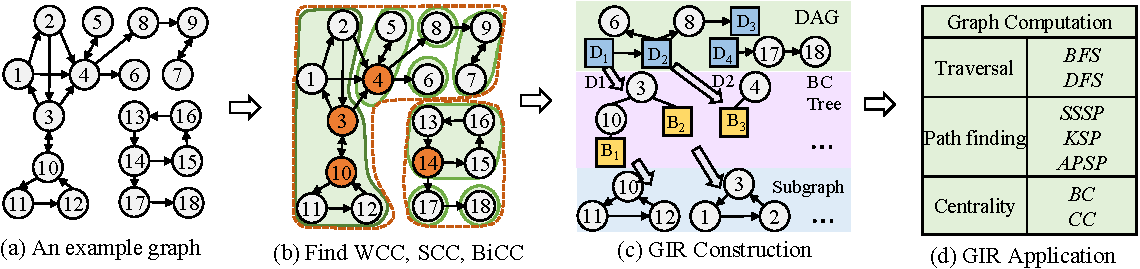
\includegraphics[width=1\linewidth]{figures/gir_framework-crop.pdf}
    \caption{Overview of the pipeline.
    (a) shows an example graph,
    (b) decomposes it into WCCs, SCCs, and BiCCs,
    (c) constructs the GIR,
    and (d) performs downstream graph query analytics on GIR.}
    \Description{Four-panel pipeline diagram: an example graph, its decomposition into WCCs/SCCs/BiCCs, the resulting GIR structure, and downstream query analytics running on GIR.}
    \label{fig:gir}
\end{figure*}

\section{Overview}
\label{sec:methodology}

% \YJ{working on.}

Figure~\ref{fig:gir} overviews the end-to-end pipeline of our method on an exmaple graph.
Particularly, 
GIR operates in three phases: GIR construction, structure-aware incremental maintenance, and GIR-enabled task parallel execution.

% GIR operates in three phases: GIR construction (Section~\ref{sec: construction}), structure-aware incremental maintenance (Section~\ref{sec: maintenance}), and GIR-enabled task parallel execution (Section~\ref{sec:task_parallel}).
% These correspond to the three technical sections that follow
% (Sections~\ref{sec:gir}, \ref{sec:maintenance}, and~\ref{sec:framework}).

% Figure~\ref{fig:gir} presents the overall workflow of \name{} using a directed graph example, covering three components: GIR construction, dynamic maintenance, and GIR-guided analytics.

% GIR is a dynamic, query-agnostic structural index that decomposes a directed graph into three nested layers, as illustrated in Figure~\ref{fig:gir}. 
\textit{(i)} For GIR construction, at the coarsest level, WCCs partition the graph into independent regions. Within each WCC, SCCs are contracted into a condensation DAG, eliminating redundant exploration of cyclic subgraphs, as shown in Figure~\ref{fig:gir}(b). Within each SCC, BiCCs and their block-cut tree expose articulation boundaries, as shown in Figure~\ref{fig:gir}(c). They enable independent processing of structurally isolated subgraphs. Together, these three layers make structural boundaries explicit and directly accessible, replacing boundaries that would otherwise be rediscovered implicitly at query time.

\textit{(ii)} To keep GIR consistent under dynamic updates, we classify every edge insertion or deletion into one of five structurally distinct cases using only pre-maintained metadata. This confines each repair to the minimum necessary region via a scope-prune-update (SPU) strategy for single-edge updates and a filter-merge-update (FMU) strategy for batches.


\textit{(iii)} GIR further unlocks task parallelism as a complement to conventional data parallelism. Because GIR decomposes the graph into independent structural units, multiple units can be processed as concurrent tasks without inter-task synchronization, offering a second dimension of parallelism that flat adjacency representations cannot provide.


% \textbf{GIR construction.} Given a directed graph, GIR decomposes it into three nested structural
% layers, Figure~\ref{fig:gir}(b)(c).
% At the coarsest level, weakly connected components (WCCs) partition the graph into globally
% independent regions.
% Within each WCC, strongly connected components (SCCs) are identified and contracted into supernodes,
% producing a condensation DAG that captures global directed reachability without cycles.
% Within each SCC, biconnected components (BiCCs) decomposition exposes articulation boundaries
% and organizes blocks into a block-cut (BC) tree.
% Figure~\ref{fig:gir}(c) shows the constructed GIR. A super vertex $D_1$ is described by a BC tree with block nodes $B_1$, $B_2$ and AP vertices 3 and 10, making explicit that any path from vertex~2 to vertex~11 must pass through both APs.
% This three-level hierarchy transforms a flat adjacency structure into
% a representation that makes structural boundaries explicit and
% directly accessible to downstream algorithms.

% % This hierarchy of WCCs, condensation DAG, and BC trees constitutes the \emph{Graph Intermediate Representation} (GIR), which materializes structural invariants once for reuse across updates and queries.

% % Given the dynamic directed graph in Figure~\ref{fig:gir}(a), \name{} first builds GIR by decomposing it into three nested structural layers.
% % At the coarsest level, the graph is partitioned into weakly connected components (WCCs).
% % Within each WCC, strongly connected components (SCCs) are identified and contracted into supernodes, producing a condensation DAG that compactly captures global inter-component reachability, as shown in Figure~\ref{fig:gir}(b).
% % At the finest level, each SCC is further decomposed into biconnected components (BiCCs) and organized as a BC tree, where block nodes correspond to BiCCs and articulation nodes correspond to articulation points (APs).

% \textbf{Structure-aware incremental maintenance.}
% When the graph evolves, GIR updates its structural layers
% incrementally rather than recomputing them from scratch.
% \textit{The key insight is that most edge insertions and deletions affect
% only a small local region of the hierarchy}.
% For each update, the designed \emph{scope-prune-update} strategy
% determines which layer is affected, restricts the repair to the
% smallest affected subregion, and performs localized structural fixes.
% For batches of updates, the designed \emph{filter-merge-update} 
% pipeline removes redundant operations and processes
% structurally related updates concurrently.


% % When the graph evolves, \name{} updates GIR incrementally rather than recomputing from scratch.
% % For each edge insertion or deletion, a \textit{scope-prune-update} (SPU) strategy first identifies which GIR layers are affected using lightweight metadata (e.g., DAG ranks), restricts repair to the smallest affected subregion, and then performs localized structural updates.
% % For batch updates, a \textit{filter-merge-update} (FMU) pipeline removes redundant operations and processes structurally related updates concurrently.

% \textbf{GIR-enabled two-level parallel execution.}
% Once GIR is updated, downstream algorithms exploit the hierarchy
% to eliminate redundant work and expose task parallelism
% (Figure~\ref{fig:gir}(d)).
% Given a source query, GIR first prunes unreachable SCCs via the
% condensation DAG.
% It then decomposes the retained region into independent BC-tree
% blocks, each of which becomes an independent task that can further improve the parallelism by enabling task parallelism.
% In the running example, five BFS tasks execute concurrently, a level of task parallelism that flat-graph traversal cannot expose.
% The same decomposition applies to other algorithms, such as SSSP, DFS, and betweenness centrality.



% Once GIR is maintained, downstream analytics exploit its hierarchy for scalable execution, as shown in Figure~\ref{fig:gir}(d).
% Given a query, \name{} prunes unreachable SCCs via the condensation DAG, decomposes the retained region into independent BC-tree blocks for concurrent task execution, and merges local results into a globally consistent output.
% In the running example, five BFS tasks execute concurrently, a level of task parallelism that flat-graph traversal cannot expose.
% The same strategy generalizes to SSSP and betweenness centrality (BC).

% \YJ{Too short. \CQ{done}}


%
%\YJ{TODO: Add the lemmas}

%\textbf{Lemma 1.}  
%Given a directed graph, after decomposing it into SCCs, all BiCCs are contained within individual SCCs.
%\textbf{Lemma 2.}  
%When an insertion occurs in the DAG layer, only nodes whose topological order lies between the affected high-level and low-level nodes may be impacted.

%\textbf{Lemma 3.}  
%During cycle detection or path verification in DAG updates, the search space can be pruned to nodes whose topological ranks lie betw  een the source and target levels.

\section{A Novel Hierarchical Graph IR}

\label{sec: construction}

% We propose GIR as a novel structural layer for dynamic graphs.
% Traditional dynamic graph systems operate directly on adjacency
% structures.
% Each downstream algorithm must repeatedly rediscover connectivity
% boundaries, articulation structure, and reachable regions from
% scratch.
% GIR instead materializes these structural properties once and
% keeps them up to date as the graph evolves.
% Downstream algorithms reuse this maintained structure rather than
% recomputing it.
% This makes GIR query-agnostic: the same structural layer serves different graph algorithms
% without any query-specific precomputation.

% \subsection{Three-Level Structural Hierarchy}
% \label{subsec:hierarchy}

GIR is built on a simple but powerful principle: \emph{separate structural organization from algorithm execution}.
However, not every structural property of a graph deserves to be maintained incrementally.
Instead, we select 
% GIR selects 
invariants that satisfy three criteria simultaneously.
First, the invariant must be \emph{incrementally maintainable}: a single
vertex/edge insertion or deletion must confine repair to the structurally
affected region, not the entire graph.
For WCC and BiCC, this region is provably local (a single component or block).
For SCC, a single edge can in principle merge many SCCs if it closes a large
cycle; however, GIR's rank-based pruning (Section~\ref{sec: maintenance})
bounds the search to the rank interval between the two endpoints, limiting the
work to the actually affected SCCs rather than triggering a global recomputation.
Second, it must be \emph{algorithm-independent}, meaning that it must reflect the structure of the graph itself, not the parameters of any
specific query.
Third, it must be \emph{directly actionable}. That is, a downstream
algorithm must be able to use it to skip work, not merely consult
it as reference.

We observe that connectivity decomposition algorithms, including WCC, SCC (along with condensation DAG), and the BC tree, 
% are 
% three standard connectivity decompositions of a directed graph that
satisfy all three criteria.
Together, they form a complete global-to-local hierarchy with no
gap and no redundancy between levels.
Motivated by this, we design the GIR as a three-level structural hierarchical layer.
% Figure~\ref{fig:gir} illustrates this hierarchy on an example graph.

\textbf{Level 1: WCC}
is chosen as it provides the strongest possible pruning
at zero traversal cost.
No path of any kind can cross a WCC boundary.
A query at any vertex is therefore entirely confined to that
vertex's WCC.
All other WCCs can be eliminated before a single edge is examined.
WCC also has the simplest incremental maintenance rule of the three. That is, one insertion can only merge two WCCs, and one deletion can only split one.
This makes the WCC layer a nearly free filter that benefits every
source-rooted algorithm on the graph.

\textbf{Level 2: SCC}
is used because it resolves the fundamental difficulty of
directed traversal, i.e., cycles.
In a directed graph, any strongly connected region is internally
equivalent for reachability purposes.
Every vertex in an SCC can reach every other vertex in the same
SCC, so the SCC as a whole can be treated as a single unit.
Contracting each SCC into a supernode and connecting them by the
remaining inter-SCC edges produces the condensation directed acyclic graph (DAG).
% which is acyclic by construction.
This transforms directed reachability into a DAG walk, eliminating
all cycle-related redundancy.
The DAG also yields a topological order that lets algorithms
process SCCs level by level without backtracking.
Incrementally, one edge insertion can at most merge SCCs by creating
a new directed cycle, and one deletion can at most split one SCC.
Both operations are local and do not affect the rest of the DAG.

\textbf{Level 3: Block-cut tree}
is selected as it exposes the finest level of independent
substructure within an SCC.
Even inside a strongly connected region, the internal topology is
not uniform.
Some vertices are articulation points (APs), whose removal will disconnect
the SCC into separate regions.
Any path between vertices in different BiCC blocks must pass through these APs.
This property holds unconditionally, regardless of algorithm type.
Therefore, we can exploit it to decompose execution. That is, each BiCC block can be
processed as an independent task, enabling task parallelism
across blocks without inter-task synchronization.
The BC tree organizes blocks and APs hierarchically, exposing the entry point of each block and making the task decomposition explicit.
% Incrementally, a single edge update typically affects only the
% block containing that edge.
% The BC tree repair is therefore confined to a small local region
% even within a large SCC.


% An algorithm that uses all three levels first discards irrelevant
% components, then navigates a cycle-free inter-SCC structure,
% then executes concurrently within independent blocks.



% Section~\ref{sec:maintenance} describes how GIR is maintained
% incrementally under continuous updates.
% Section~\ref{sec:framework} describes how downstream algorithms
% exploit the hierarchy for parallel and efficient computation.

% \subsection{Scope of Benefit}
% GIR is most beneficial for algorithms whose execution can be pruned, decomposed, or reordered using structural boundaries. 
% The three GIR levels provide three types of structural knowledge that enable three corresponding optimizations.

% \textit{WCC (Level 1) is for scope elimination}. Any single-source algorithm on a directed or undirected graph can immediately discard all WCCs that do not contain the source. This benefits many algorithms, such as, BFS, DFS, SSSP, APSP (per-source), reachability queries, betweenness centrality (which issues SSSP from every vertex), $k$-shortest paths. Essentially any algorithm that starts from a specific source benefits.

% \textit{Condensation DAG (Level 2) is for cycle elimination.} On a directed graph, any algorithms that must follow directed paths can use the DAG to prune reachable SCCs before walking raw edges. This benefits algorithms, such as SSSP, directed reachability, topological-order-dependent algorithms, and dependency-chain analysis. Algorithms that need to traverse only forward-reachable SCCs can skip cycles entirely.

% \textit{BC tree (Level 3) is for task decomposition}. Any algorithms that can process subgraphs independently and then merge results benefits. This is the basis of GIR's task parallelism contribution. BFS, DFS, SSSP, and betweenness centrality all have this property. The BC tree also enables localized updates, i.e., when GIR is maintained after an edge change, only the affected BiCC block needs to be repaired.

% % GIR is most beneficial for algorithms that issue queries from
% % a specific source or target, or that traverse directed paths.
% % This class includes BFS, DFS, SSSP, all-pairs shortest paths
% % (via per-source SSSP), betweenness centrality, closeness
% % centrality, reachability queries, and k-shortest paths.
% % For these algorithms, GIR enables two distinct optimizations.
% % First, WCC and DAG structure prune the search space before
% % traversal begins.
% % Second, BC-tree decomposition exposes task parallelism across
% % independent BiCC blocks.

% Algorithms that aggregate globally across all vertices, such
% as PageRank~\cite{page1999pagerank} and label propagation~\cite{zhu2002learning}, might not directly benefit from the
% condensation DAG or BC tree.
% They operate on all edges regardless of source, so
% structural boundaries do not reduce their work.
% However, these algorithms still benefit from WCC-level
% partitioning. That is, separating WCCs can be processed independently
% and in parallel.
% After that, the updates confined to one WCC require
% only that component's scores to be updated.
% We would not claim of benefit for global aggregation algorithms beyond this.

%\textbf{GIR design.}
% We propose GIR as a hierarchical graph intermediate representation built upon three fundamental decompositions: weakly connected components (WCCs), strongly connected components (SCCs), and biconnected components (BiCCs)~\cite{tarjan1972depth, tarjanscc1972depth, hopcroft1973algorithm,ji2018ispan,ji2020aquila}.
% As illustrated in Section~\ref{sec:methodology}, these form three nested structural layers---WCCs, the SCC condensation DAG, and per-SCC BC trees---that together make connectivity structure explicit and reusable.
% Here we focus on three design aspects that are not covered in the overview: structural--execution separation, storage compatibility, and extensibility.


% \subsection{old}
% A key feature of GIR is that it separates \emph{structural organization} from \emph{algorithm execution}.
% Traditional dynamic graph processing often operates directly on adjacency structures, forcing each downstream task to repeatedly rediscover connectivity boundaries, critical connectors, and affected regions.
% In contrast, GIR materializes these structural invariants once and reuses them across multiple tasks.
% For example, the condensation DAG can be used to prune unreachable SCCs during traversal or path computation, while the BC tree can localize exploration to only those BiCCs and articulation boundaries that are relevant to a given query.
% This makes GIR query-agnostic: the same structural representation can support many different downstream computations, such as reachability, traversal, and path finding~\cite{tarjan1972depth,gross2005graph,nagamochi2000graph}, without requiring each algorithm to rebuild structural knowledge from scratch.

% Another important aspect of GIR is that its hierarchy naturally supports scalable execution.
% The WCC, SCC, and BiCC layers form explicit structural partitions that can be used as independent or semi-independent computation units.
% At the global level, different WCCs can often be processed separately.
% Within a WCC, SCC supernodes provide a compact execution scope for many graph tasks.
% Within an SCC, BiCCs and articulation points further expose localized substructures that can be processed selectively.
% This hierarchical decomposition is particularly suitable for multi-threaded and GPU systems, where component-level parallelism and localized memory access are critical for performance.
% Our previous systems, Aquila~\cite{ji2020aquila} and iSpan~\cite{ji2018ispan,ji2022ispan}, already demonstrate that WCC, SCC, and BiCC decompositions can be computed at high throughput on billion-edge graphs, which makes GIR a practical foundation for large-scale dynamic graph analytics.

% GIR is also designed to work with dynamic graph storage rather than replacing it.
% The representation can be integrated with existing dynamic graph formats such as PMA~\cite{bender2007adaptive}, DCSR~\cite{king2016dynamic}, Terrace~\cite{pandey2021terrace}, and DGAP~\cite{islam2023dgap}.
% In this sense, GIR serves as a structural layer above the underlying storage layer: the storage format is responsible for maintaining graph data efficiently under updates, while GIR is responsible for exposing reusable structural invariants for analytics and maintenance.
% This separation improves modularity and allows GIR to be incorporated into existing dynamic graph systems without redesigning the entire storage stack.

% Although the current instantiation of GIR focuses on WCC, SCC, and BiCC, the framework itself is intentionally extensible.
% These three decompositions are the core structural primitives in our current design because they provide a strong balance between expressiveness, computability, and practical usefulness.
% However, the abstraction is not limited to them.
% Additional structural indices or auxiliary representations, such as dominator trees or reachability indices, can be incorporated whenever they provide value for dynamic maintenance or downstream analytics.
% This makes GIR a general structural framework for dynamic graph systems rather than a fixed-purpose representation.

% Overall, GIR transforms a flat dynamic graph into a layered structural representation that explicitly captures both global connectivity and local articulation structure.
% By organizing the graph into reusable WCC, SCC, and BC tree layers, GIR provides a common framework for structural maintenance, query pruning, and scalable downstream computation.
% This hierarchical design is the key that allows GIR to support efficient updates while also accelerating diverse graph analytics.

% \YJ{Example}
% In Figure~\ref{fig:pre_process}, nodes prefixed with `a' denote APs, and nodes prefixed with `b' denote BiCCs. There are two important properties of the BC tree that lay the foundation for us to exploit it to KSP computation:
% These BiCCs serve as logical submodules that support efficient localized computation and resilience analysis. The BC tree structure not only enables rapid evaluation of queries like fault impact or neighborhood exploration, but also allows future integration of fine-grained update strategies on a per-block basis.
% \YJ{Explain our BC+ tree idea.}
% \YJ{Can add the lemma of AP in SCC here.}



\section{Structure-Aware Incremental Maintenance}
\label{sec: maintenance}



\subsection{Structural Classification of Edge Updates}




As the graph dynamically inserts or deletes vertices or edges, this may affect GIR layers in different ways.
However, we observe that many updates actually leave the structural connectivity entirely unchanged. For example, an edge inserted within a WCC would not alter that WCC at all. 
% For example, an edge inserted within a WCC would not alter that WCC at all.

To leverage this opportunity, we design a \textit{structure-aware incremental maintenance method to identify exactly which regions are affected and repair only the minimum necessary ones}.
% To address it, we design two complementary strategies, i.e., \textit{Scope-Prune-Update (SPU) for single update}, and \textit{Filter-Merge-Update (FMU) for batch update}.
Particularly, GIR's three-layer hierarchy transforms the maintenance problem.
Instead of treating every edge change as a potential graph-wide event, \textit{we classify each update into one of five distinct cases using only pre-maintained metadata}.
Each case identifies exactly which layers are affected and confines the repair to the smallest possible region.
We call this strategy \textit{Scope-Prune-Update (SPU)} for single-edge updates and extend it to \textit{Filter-Merge-Update (FMU)} for batches.

We primarily focus on \textit{single edge update} (insertion or deletion), as vertex insertions without edges do not affect connectivity and vertex deletions reduce to bulk edge deletions.
The central challenge is determining which GIR layers each operation affects.
Because GIR stores component labels, SCC membership, DAG ranks, and articulation point metadata for every vertex, it resolves this question through a metadata lookup, not a graph traversal.
This classification is only possible as GIR maintains all three structural layers simultaneously.
% No system that lacks these layers can make such a distinction.
% \YJ{working on.}

Every edge update ($s\rightarrow t$) falls into one of five cases shown in Figure~\ref{fig:scope-update}.
Particularly, \circled{c1}~$s$ and $t$ reside in \emph{different WCCs} (insertion);
\circled{c2}~$s$ and $t$ reside in the \emph{same WCC but different SCCs} (insertion);
\circled{c3}~$s$ and $t$ reside in the \emph{same SCC but different BiCCs} (insertion);
\circled{c4}~$s$ and $t$ reside in the \emph{same BiCC} (insertion);
\circled{c5}~edge \emph{deletion}, whose scope depends on bridge status.
In addition, Table~\ref{tab:updates} summarizes the scope rules and time complexity.
For each case, we identify which GIR layers are affected (\textit{scope}), how GIR restricts computation to the smallest subgraph (\textit{prune}), and what structural repair GIR performs (\textit{update}). 
% Below, we will discuss the details for each case.

\begin{figure}[t]
    \centering
    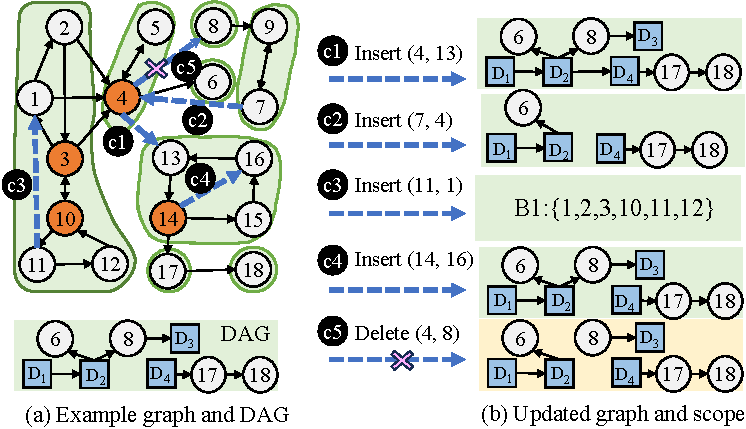
\includegraphics[width=1\linewidth]{figures/update_scope-crop.pdf}
    \caption{Five cases (\circled{c1}-\circled{c5}) for a single edge update.
    % Cases \circled{c1}-\circled{c4} are about insertions,
    % % classified by the structural relationship between the two endpoints; 
    % while \circled{c5} is about deletion.
    % classified by whether the removed edge is a bridge and at which GIR layer.
    Affected DAG nodes are highlighted in blue, and green shade indicates a WCC.}
    % \YJ{X on the deletion edge.}}
    \label{fig:scope-update}
\end{figure}


\begin{table}[t]
    \centering
    % \footnotesize
    \setlength{\tabcolsep}{3pt}
    % \renewcommand{\arraystretch}{1.1}
    \caption{Scope rules and SPU time complexity per case.
    $|V_{\mathrm{a}}|$ and $|E_{\mathrm{a}}|$ denote the number of vertices and edges in the affected region;
    $\Delta r$ denotes the rank interval for Case~2.}
    \begin{tabular}{c l c l l}
    \toprule
    \textbf{Case} & \textbf{Endpoint relation} & \textbf{Op} & \textbf{Layers} & \textbf{Complexity} \\
    \midrule
    1  & Different WCCs                         & Ins & WCC             & $\mathcal{O}(1)$ \\
    \multirow{2}{*}{2}
       & \multirow{2}{*}{Same WCC, diff.\ SCCs} & \multirow{2}{*}{Ins}
                                                & SCC (no cycle)  & $\mathcal{O}(1)$ \\
       &                                        &     & SCC+BiCC        & $\mathcal{O}(\Delta r$+$|V_{\mathrm{a}}|$+$|E_{\mathrm{a}}|$) \\
    3  & Same SCC, diff.\ BiCCs                 & Ins & BiCC            & $\mathcal{O}(|V_{\mathrm{a}}|+|E_{\mathrm{a}}|)$ \\
    4  & Same BiCC (no-op)                      & Ins & BiCC             & $\mathcal{O}(1)$ \\
    \midrule
    5a & Non-bridge                             & Del & BiCC            & $\mathcal{O}(|V_{\mathrm{a}}|+|E_{\mathrm{a}}|)$ \\
    5b & Bridge within SCC                      & Del & SCC+BiCC        & $\mathcal{O}(|V_{\mathrm{a}}|+|E_{\mathrm{a}}|)$ \\
    5c & Bridge in DAG                          & Del & WCC+BiCC        & $\mathcal{O}(|V_{\mathrm{a}}|+|E_{\mathrm{a}}|)$ \\
    \bottomrule 
    \end{tabular}
    \label{tab:updates}
\end{table}


\textbf{Case 1 (Insertion): $s$ and $t$ reside in different WCCs.}
The inserted edge connects two previously disconnected regions.
No directed cycle can form across WCC boundaries, and thus no biconnected structure inside either component changes.

\textit{Scope.} GIR identifies WCC layer as the only affected layer.

\textit{Prune and Update.} GIR merges the two components in $O(1)$ time via a
union-find root-pointer update~\cite{tarjan1975efficiency}: only the root label
of the smaller component is redirected to the root of the larger one, with no
SCC or BC tree traversal.
Full path compression is applied lazily during subsequent label lookups, keeping
amortized per-operation cost at $O(\alpha(n))$.
% \CQ{The time complexity is $\mathcal{O}(1)$, as the merge requires only a single WCC label update with no SCC or BiCC traversal.}


\textit{Example.}
Inserting an edge $(4,\,13)$ (\circled{c1} in Figure~\ref{fig:scope-update})
% (\circled{c1}) 
bridges $\text{WCC}_1 = \{1, ..., 12\}$ and $\text{WCC}_2 = \{13, ..., 18\}$.
Thus, GIR connects the two condensation DAGs into one.





\textbf{Case 2 (Insertion): $s$ and $t$ are in the same WCC but different SCCs.}
The inserted edge $s \to t$ introduces a new edge between two SCC supernodes in the condensation DAG.
The critical question is \textit{whether this edge creates a directed cycle, which would cause two or more SCCs to merge}.

\textit{Scope.} To answer this without traversing the entire DAG, we design a rank-based method. 
That is, we assign each SCC a {rank}, which is a compact topological index maintained incrementally alongside the DAG.
If $\mathrm{rank}(\mathrm{SCC}(s)) \le \mathrm{rank}(\mathrm{SCC}(t))$, the edge either follows the existing DAG order or connects two SCCs at the same rank with no directed path between them.
Neither will form a cycle, and the scope is limited to inserting a new DAG edge with no SCC-level structural change.
If $\mathrm{rank}(\mathrm{SCC}(s)) > \mathrm{rank}(\mathrm{SCC}(t))$, the edge goes against the DAG order and may introduce a cycle.
The scope then expands to the SCC and BiCC layers.

\textit{Prune.} 
% As illustrated in Figure~\ref{fig:rank-prune},
GIR restricts cycle detection to the rank interval $[\mathrm{rank}(\mathrm{SCC}(t)),\,\mathrm{rank}(\mathrm{SCC}(s))]$ in the  DAG.
This avoids a global DAG search.

\textit{Update.} If a cycle is detected within this interval, it merges all SCCs on this cycle, updates the condensation DAG locally, and reconstructs the BC trees of the affected SCCs. The time complexity is $\mathcal{O}(\Delta r + |V_{\mathrm{a}}| + |E_{\mathrm{a}}|)$, where $|V_{\mathrm{a}}|$ and $|E_{\mathrm{a}}|$ denote vertex and edge count of  the affected region, and $\Delta r$ denotes the rank interval.
If no cycle forms, the cost is $\mathcal{O}(1)$. 

% When a cycle is detected, the rank-interval search costs $\mathcal{O}(\Delta r)$ and the SCC merge plus BC tree reconstruction costs $\mathcal{O}(|V_{\mathrm{aff}}| + |E_{\mathrm{aff}}|)$, giving a total of $\mathcal{O}(\Delta r + |V_{\mathrm{aff}}| + |E_{\mathrm{aff}}|)$.

\textit{Example.}
As shown in Figure~\ref{fig:rank-prune}, inserting edge $(7,\,4)$ (\circled{c2}) has $\mathrm{rank}(D_3) > \mathrm{rank}(D_2)$. As $D_2 \to D_3$ is in the original DAG, the edge goes against the DAG order and triggers cycle detection over $[\mathrm{rank}(D_2),\,\mathrm{rank}(D_3)]$.
A cycle is found, and $D_2$ and $D_3$ will be merged.
The BC tree of the combined SCC will be updated, as shown in Figure~\ref{fig:scope-update} (\circled{c2}).
In contrast, inserting $(2,\,8)$ satisfies $\mathrm{rank}(\mathrm{SCC}(2)) \le \mathrm{rank}(\mathrm{SCC}(8))$, thus no cycle can form and only a new DAG edge is added.



\textbf{Case 3 (Insertion): $s$ and $t$ are in the same SCC but different BiCCs.}
Both endpoints lie within the same SCC, so no WCC or SCC needs to be changed.

\textit{Scope.} GIR confines the scope to the BiCC layer. Specifically, only the two BiCC blocks containing $s$ and $t$ are potentially affected.

\textit{Prune and Update.} The new edge may merge the two blocks into a single larger BiCC, eliminating one or more APs.
GIR updates the BC tree accordingly.
The time complexity is $\mathcal{O}(|V_{\mathrm{a}}| + |E_{\mathrm{a}}|)$, confined to the two affected BiCC blocks and the local BC tree repair.

\begin{figure}[t]
    \centering
    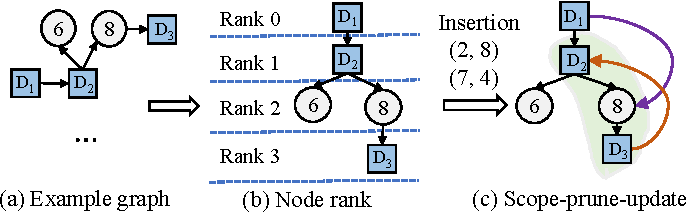
\includegraphics[width=1\linewidth]{figures/scope_update-crop.pdf}
    \caption{Rank-interval pruning for Case \circled{c2} (inter-SCC insertion). 
    Inserting edge (2, 8) will not affect SCC, while edge (7, 4) will merge multiple SCCs.
    % Each SCC is assigned a topological rank in the condensation DAG. When an inserted edge goes against the DAG order from $\mathrm{SCC}(s)$ to $\mathrm{SCC}(t)$, GIR restricts cycle detection to the rank interval $[\mathrm{rank}(\mathrm{SCC}(t)),\,\mathrm{rank}(\mathrm{SCC}(s))]$ (shaded region), avoiding a global DAG traversal.
    %\YJ{Make sure this figure matches with the example in Figure 5.} done it;s the same
    }
    \label{fig:rank-prune}
\end{figure}
\textit{Example.}
Inserting an edge $(11,\,1)$ (\circled{c3} in Figure~\ref{fig:scope-update}) will lead to the merge of two blocks. Particularly, 
vertex $11$ is in block $B_1 = \{10,\,11,\,12\}$ and vertex $1$ is in block $B_2 = \{1,\,2,\,3\}$, both within $D_1$.
Therefore, GIR merges the two blocks into $B_1 = \{1,\,2,\,3,\,10,\,11,\,12\}$.
% , as shown in Figure~\ref{fig:scope-update} (\circled{c3}).


\textbf{Case 4 (Insertion): $s$ and $t$ are in same BiCC.}
As both vertices already belong to the same BICC, adding an edge within an already 2-edge-connected subgraph will not create new APs, split any BiCC, or alter SCC or WCC structure.

\textit{Scope.} GIR identifies the update as a structural no operation for all layers.
The time complexity is $\mathcal{O}(1)$.
% and no maintenance is needed.
% \CQ{Since no structural change occurs, the time complexity is $\mathcal{O}(1)$.}


\textit{Example.}
Inserting an edge $(14,\,16)$ (\circled{c4} in Figure~\ref{fig:scope-update}) will not change the GIR as both vertices lie in the same block $D_4$.
% so the GIR remains unchanged (Figure~\ref{fig:scope-update}, \circled{c4}).

\textbf{Case 5 (Deletion):}
The scope of deleting an edge $(s,\,t)$
depends on whether the edge is a bridge, which is defined as the only edge between two blocks.
%\YJ{clearly explain what is an bridge.} 
For this case, GIR further decomposes it into three sub-cases.


\emph{Case 5a (non-bridge):}
If parallel edges or alternative undirected paths exist between $s$ and $t$, the deletion cannot change WCC, SCC, or higher-level connectivity.
GIR confines the scope to the BiCC layer, checks whether any articulation points have changed, and repairs the BC tree locally within the enclosing SCC.
% \CQ{
The time complexity is $\mathcal{O}(|V_{\mathrm{a}}| + |E_{\mathrm{a}}|)$, confined to the affected BiCC block within the enclosing SCC.
% }


% \emph{Case 5a (non-bridge):}
% If parallel edges or alternative undirected paths exist between $s$ and $t$, the deletion cannot change WCC, SCC, or higher-level connectivity.
% \textit{Scope.} GIR confines the scope to the BiCC layer: the removed edge may alter block boundaries or articulation structure within the enclosing SCC, but the change does not propagate upward.
% \textit{Update.} GIR checks whether any articulation points have changed and repairs the BC tree locally.

\emph{Case 5b (bridge within an SCC):}
% If the edge is the unique undirected path between its endpoints and both endpoints share the same SCC, the deletion may split that SCC.
% \textit{Scope.} GIR expands the scope to the SCC layer: it checks whether the directed SCC breaks apart.
% If so, GIR partitions the affected SCC, rebuilds the relevant fragment of the condensation DAG, and reconstructs the BC trees of the resulting components.
If the edge is a bridge and both endpoints share the same SCC, GIR expands the scope to the SCC layer.
It checks whether the directed SCC breaks apart and, if so, partitions the affected SCC, rebuilds the relevant fragment of the condensation DAG, and reconstructs the BC trees of the resulting components.
% \CQ{
The time complexity is $\mathcal{O}(|V_{\mathrm{a}}| + |E_{\mathrm{a}}|)$, covering the SCC partition check, condensation DAG fragment update, and BC tree reconstruction.

\emph{Case 5c (bridge in the condensation DAG):}
If the deleted edge is an inter-SCC edge and serves as the bridge connecting two regions of the WCC, its removal disconnects the WCC entirely.
In this situtation, both WCC and BiCC layers are affected. It will split the WCC into two independent components, partition the condensation DAG accordingly, and update the BC trees on each side to reflect the new component boundaries.
The time complexity is $\mathcal{O}(|V_{\mathrm{a}}| + |E_{\mathrm{a}}|)$, covering the WCC split, condensation DAG partition, and BC tree updates on both resulting components.

\textit{Example.} 
The edge $4 \to 8$ (\circled{c5} in Figure~\ref{fig:scope-update}) 
% Deleting bridge $(4,\,8)$ (\circled{c5}): edge $4 \to 8$ 
is the only edge between the $\{D_1, D_2\}$ side and the $\{6, 8, D_3\}$ side.
% of the graph.
Deleting it will split the WCC into two, which will lead to WCC relabeling and BC tree updating on each resulting component.
% \CQ{

% }



% \emph{Case 5c (bridge in the condensation DAG):}
% If the deleted edge is an inter-SCC arc and serves as the only undirected path connecting two regions of the WCC, its removal disconnects the WCC entirely.

% \textit{Scope.} GIR identifies both the WCC and BiCC layers as affected: it splits the WCC into two independent components, partitions the condensation DAG accordingly, and updates the BC trees on each side to reflect the new component boundaries.

% \textit{Example.}
% Deleting bridge $(4,\,8)$ (\circled{c5}): edge $4 \to 8$ is the only undirected path between the $\{D_1, D_2\}$ side and the $\{6, 8, D_3\}$ side of the graph.
% GIR splits the WCC into two components, as shown in Figure~\ref{fig:scope-update} (\circled{c5}), and performs WCC relabeling and BC tree updates on each resulting component.


% \textit{Example.}
% Deleting bridge $(4,\,8)$ (\circled{c5}): edge $4 \to 8$ is the only undirected path between the $\{D_1, D_2\}$ side and the $\{6, 8, D_3\}$ side of the graph.
% GIR splits the WCC into two components, as shown in Figure~\ref{fig:scope-update} (\circled{c5}), and performs WCC relabeling and BC tree updates on each resulting component.




%if 5 == all, all the edges are included, insertion and deletion are within those cases.

% Table~\ref{tab:updates} summarizes the scope rules and per-case time complexity.
% \CQ{Three cases cost $\mathcal{O}(1)$: Case~1 (WCC merge) requires only a label update; Case~2 without a cycle adds a single DAG edge; Case~4 is a structural no-op that touches no GIR layer.
% Case~2 with a cycle costs $\mathcal{O}(\Delta r + |V_{\mathrm{aff}}| + |E_{\mathrm{aff}}|)$, where $\Delta r$ bounds the rank-interval cycle search and $|V_{\mathrm{aff}}| + |E_{\mathrm{aff}}|$ covers the SCC merge and BC tree reconstruction within the identified interval.
% Cases~3, 5a, 5b, and 5c all cost $\mathcal{O}(|V_{\mathrm{aff}}| + |E_{\mathrm{aff}}|)$, where the affected region is always confined to the structurally identified subgraph: the two BiCC blocks for Case~3, the enclosing BiCC block for Case~5a, the affected SCC and its condensation DAG fragment for Case~5b, and both resulting WCC components with their BC trees for Case~5c.
% Crucially, $|V_{\mathrm{aff}}| + |E_{\mathrm{aff}}|$ is always a strict subgraph of $G$, so SPU never performs a full-graph traversal regardless of graph size.}

% \subsection{Region-Minimal Layered Repair}

% \subsection{Top-down Cascaded Repair}

% The five-case classification identifies \emph{which} layers are affected. 
% % tells GIR \emph{which} layers are affected.
% The follow-up challenge is to correctly apply them on the GIR.
% To achieve that, we design a top-down cascaded repair method 
% % reginon-minimal layered repair method 
% to confine and execute the repair to guarantee that no update touches more structure than logically necessary.

% The key design principle is \textbf{top-down cascaded repair}, i.e., GIR always repairs layers from coarsest to finest.
% It first stabilizes the WCC layer, then the SCC/DAG layer, then the BiCC/BC tree layer.
% Each layer's repair is confined to the region that the layer above it identifies as affected.
% This cascade ensures that lower-layer repairs never operate on stale higher-layer state.

% \textit{WCC-layer repair.}
% WCC repair is the simplest.
% For Case~1 insertions, GIR merges two WCCs with a single relabeling step.
% For Case~5c deletions, GIR splits a WCC by checking connectivity and assigning new component labels.
% Both operations are $O(1)$ or $O(|V_{\mathrm{WCC}}|)$ in the affected component.
% No other case triggers WCC repair.

% \textit{SCC/DAG-layer repair.}
% SCC repair is governed by cycle formation (insertion) or cycle breaking (deletion).
% For Case~2, the rank-interval pruning (Figure~\ref{fig:rank-prune}) bounds the cycle search to a small region of the condensation DAG.
% If GIR finds a cycle, it merges the involved SCCs and locally updates the DAG.
% For Case~5b, GIR checks whether the deleted bridge disconnects the directed SCC.
% If so, GIR partitions the SCC, updates the DAG fragment, and passes the resulting sub-SCCs to the BiCC layer for BC tree reconstruction.
% In both cases, GIR touches only the SCCs within the pruned interval, not the entire DAG.

% \textit{BiCC/BC tree repair.}
% BiCC repair runs only after the WCC and SCC layers have stabilized.
% For Case~3, GIR merges the two affected BiCC blocks and removes the eliminated articulation points from the BC tree.
% For Cases~5a and 5b, GIR checks whether the deletion creates new articulation points or splits existing blocks, and repairs the BC tree accordingly.
% Because the higher layers have already localized the affected SCC, BC tree repair is confined to a small subgraph.
% Within a large SCC, GIR can carry out multiple non-overlapping BiCC repairs in parallel.

% This layered discipline produces a strong guarantee, that the repair never performs more  than the structural change requires.

\subsection{Filter-Merge-Update for Batch Updates}

Applying the single edge update strategy (SPU) independently to each update in a batch is correct but inefficient.
% Two problems arise.
There are two problems.
\textit{(i)} Some updates cancel or are redundant. That is, if an edge is inserted and later deleted within the same batch, neither needs to be processed.
\textit{(ii)} Multiple updates may jointly affect the same structural region.
Processing them one at a time triggers repeated maintenance on the same region.

To address both problems, 
we design a filter-merge-update (FMU) strategy by preprocessing the batch before applying SPU logic. Specifically, it involves three stages.

\textit{(i) Filter} stage removes updates that does not require processing.
Particular, we identify two such types of updates.
The first is canceling pair. 
% \emph{Canceling pairs:} 
That is, if an edge is inserted and later deleted within the same batch (or vice versa), the two operations cancel and GIR discards both.
The second is structural no operations.
% \emph{Structural no-ops:} 
Particularly, based on the five-case classification
% each remaining update using the five-case rules
in Table~\ref{tab:updates}, we remove any Case~4 updates (i.e., $s$ and $t$ are in the same BiCC), as they will not affect any GIR layer.
% Particularly, GIR classifies each remaining update using the five-case rules in Table~\ref{tab:updates} and removes any Case~4 updates (i.e., $s$ and $t$ are in the same BiCC) immediately, since they cannot affect any GIR layer.
This filter step reduces both the number of updates and the total maintenance work.

\textit{(ii) Merge}
% After filtering, GIR 
will group the remaining updates by the structural region they may jointly affect.
We first group the updates whose endpoints share the same WCC.
Within each WCC group, we identify updates whose SCC endpoints have overlapping DAG rank intervals and merges them into a single SCC-level maintenance region.
Further, we group updates that touch the same local articulation structure at the BiCC level.
This grouping has two benefits.
First, it amortizes repeated maintenance. That is, the updates that would trigger repairs on the same region are handled together in a single pass.
Second, it identifies structurally independent groups, each of which becomes a natural unit for parallel execution.

\textit{(iii) Update.}
Finally, GIR applies the single edge update logic to each merged region rather than to individual edges.
A set of inserted edges may jointly create a cycle and merge several SCCs, even though none of the edges alone would trigger a merge.
GIR detects such structural transitions over the merged region and repairs the corresponding WCC, SCC, and BC tree structures in a coordinated way.
Once the batch is complete, GIR processes independent merged regions concurrently.
This makes FMU a parallel and amortized extension of SPU for high-throughput update streams.

% Together, SPU and FMU keep GIR structurally consistent under both fine-grained and high-throughput updates.





% % As the graph will dynamically insert or delete nodes or edges, this may affect GIR layers in different ways.
% % % edge insertion or deletion may affect GIR layers in different ways.
% % However, we observe that many updates actually leave the structural connectivity entirely unchanged. For example, an edge inserted within a WCC would not after that WCC at all. 
% % To leverage this opportunity, \textit{the key challenge is to identify exactly which layers are affected and repair only the minimum necessary region}.
% % To address it, we design two complementary strategies, i.e., \textit{Scope-Prune-Update (SPU) for single update}, and \textit{Filter-Merge-Update (FMU) for batch update}.
% % We detail each strategy below.

% % Following the SPU and FMU strategies outlined in Section~\ref{sec:methodology}, \name{} updates GIR incrementally after each graph change.
% % The central challenge is that an edge insertion or deletion may affect GIR layers in different ways, and many updates leave the structural connectivity entirely unchanged.
% % We now detail how each strategy is realized.

% %\YJ{TODO: How do we dynamically update the GIR? Please write as much details as possible}

% % \subsection{Scope-Prune-Update for Single Update}

% \subsection{Accurately Locating Affected Regions}

% % \YJ{Please read the following and think about plotting a figure.}

% \begin{figure}
%     \centering
%     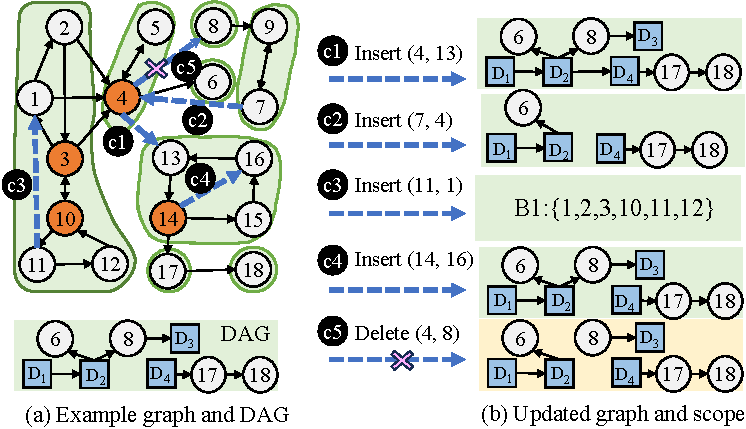
\includegraphics[width=1\linewidth]{figures/update_scope-crop.pdf}
%     \caption{Five scope cases (\circled{c1}--\circled{c5}) for a single edge update on the running example.
%     Cases \circled{c1}--\circled{c4} cover insertions classified by the structural relationship between the
%     two endpoints; \circled{c5} covers deletion, classified by whether the removed edge
%     is a bridge and at which GIR layer.
%     Affected DAG nodes are highlighted in blue; yellow shading indicates a WCC split.}
%     \label{fig:scope-update}
% \end{figure}

% We focus on \textit{single edge update} (insertion/deletion), as node insertions without edges
% do not affect connectivity and node deletions reduce to bulk edge deletions.
% The central challenge is determining which GIR layers are affected by each operation.
% Because GIR stores component labels, SCC membership, DAG ranks, and articulation-point
% metadata for every vertex, this classification requires no graph traversal.
% As illustrated in Figure~\ref{fig:scope-update}, every edge update falls into one of five cases:
% \circled{c1}~$s$ and $t$ reside in \emph{different WCCs} (insertion);
% \circled{c2}~$s$ and $t$ reside in the \emph{same WCC but different SCCs} (insertion);
% \circled{c3}~$s$ and $t$ reside in the \emph{same SCC but different BiCCs} (insertion);
% \circled{c4}~$s$ and $t$ reside in the \emph{same BiCC} (insertion);
% \circled{c5}~edge \emph{deletion}, whose scope depends on bridge status.

% \textbf{Case 1 (Insertion): $s$ and $t$ belong to different WCCs.}
% The inserted edge connects two previously disconnected regions.
% No directed cycle can form across WCC boundaries, and no articulation structure inside
% either component changes.
% The scope is confined to the WCC layer: the two components are merged with an $O(1)$
% label update, and neither the SCC condensation DAGs nor the BC trees are touched.
% \textit{Example.}
% Inserting edge $(4,\,13)$ (\circled{c1}) bridges WCC$_1 = \{1\text{--}12\}$ and
% WCC$_2 = \{13\text{--}18\}$.
% The two condensation DAGs are concatenated into a single one, as shown in
% Figure~\ref{fig:scope-update} (\circled{c1}).

% \begin{figure}[t]
%     \centering
%     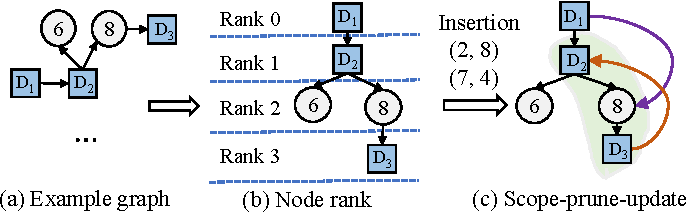
\includegraphics[width=1\linewidth]{figures/scope_update-crop.pdf}
%     \caption{Rank-interval pruning for Case \circled{c2} (inter-SCC insertion).
%     Each SCC is assigned a topological rank in the condensation DAG.
%     When an inserted edge goes against the DAG order from $\mathrm{SCC}(s)$ to
%     $\mathrm{SCC}(t)$, cycle detection is confined to the rank interval
%     $[\mathrm{rank}(\mathrm{SCC}(t)),\,\mathrm{rank}(\mathrm{SCC}(s))]$
%     (shaded region), avoiding a global DAG traversal.}
%     \label{fig:rank-prune}
% \end{figure}

% \textbf{Case 2 (Insertion): $s$ and $t$ are in the same WCC but different SCCs.}
% The inserted edge $s \to t$ introduces a new arc between two SCC supernodes in the
% condensation DAG.
% The critical question is whether this arc creates a directed cycle, which would cause
% two or more SCCs to merge.
% To answer this without traversing the entire DAG, GIR assigns each SCC a \emph{rank}—a
% compact topological index maintained incrementally alongside the condensation DAG.
% If $\mathrm{rank}(\mathrm{SCC}(s)) < \mathrm{rank}(\mathrm{SCC}(t))$, the edge follows
% the existing DAG order and cannot close a cycle; the scope is limited to inserting a
% new DAG arc with no SCC-level structural change.
% If $\mathrm{rank}(\mathrm{SCC}(s)) > \mathrm{rank}(\mathrm{SCC}(t))$, the edge goes
% against the DAG order and may introduce a cycle.
% As illustrated in Figure~\ref{fig:rank-prune}, GIR restricts cycle detection to the
% rank interval $[\mathrm{rank}(\mathrm{SCC}(t)),\,\mathrm{rank}(\mathrm{SCC}(s))]$ in
% the condensation DAG, avoiding a global DAG search.
% If a cycle is confirmed within this interval, all SCCs on the cycle are merged, the
% condensation DAG is updated locally, and the BC trees of the affected SCCs are
% reconstructed.
% \textit{Example.}
% Inserting edge $(5,\,2)$ (\circled{c2}): vertex $5 \in D_2$ and vertex $2 \in D_1$, with
% $\mathrm{rank}(D_2) > \mathrm{rank}(D_1)$ because $D_1 \to D_2$ in the original DAG.
% The edge goes against the DAG direction, so GIR runs cycle detection restricted to the
% interval $[\mathrm{rank}(D_1),\,\mathrm{rank}(D_2)]$ (Figure~\ref{fig:rank-prune}).
% A cycle is confirmed; $D_1$ and $D_2$ are merged, and the BC tree within the new
% combined SCC is updated, as shown in Figure~\ref{fig:scope-update} (\circled{c2}).

% \textbf{Case 3 (Insertion): $s$ and $t$ are in the same SCC but different BiCCs.}
% Both endpoints lie within the same SCC, so no WCC or SCC membership can change.
% The scope is confined to the BiCC layer: specifically, only the two BiCC blocks
% containing $s$ and $t$ are potentially affected.
% The new edge may merge the two blocks into a single larger BiCC, eliminating one or
% more articulation points and updating the BC tree accordingly.
% \textit{Example.}
% Inserting edge $(11,\,1)$ (\circled{c3}): vertex $11$ is in block $b_1 = \{10,\,11,\,12\}$ and
% vertex $1$ is in block $b_2 = \{1,\,2,\,3\}$, both within $D_1$.
% The two blocks merge into $b_1 = \{1,\,2,\,3,\,10,\,11,\,12\}$, as shown in
% Figure~\ref{fig:scope-update} (\circled{c3}).

% \textbf{Case 4 (Insertion): $s$ and $t$ are in the same BiCC.}
% Both endpoints already belong to the same biconnected component.
% Adding an edge within an already 2-edge-connected subgraph cannot create new
% articulation points, split any BiCC block, or alter SCC or WCC structure.
% The update is a structural no-op for all GIR layers; no maintenance is needed.
% \textit{Example.}
% Inserting edge $(14,\,16)$ (\circled{c4}): both vertices lie in the same BiCC block of $D_4$, so
% the GIR remains unchanged (Figure~\ref{fig:scope-update}, \circled{c4}).

% \textbf{Case 5 (Deletion):}
% For deletion of edge $(s,\,t)$, the scope depends on whether the edge is a bridge—
% the sole undirected path between its two endpoints.

% \emph{Case 5a (non-bridge):}
% If parallel edges or alternative undirected paths exist between $s$ and $t$, the
% deletion cannot change WCC, SCC, or higher-level connectivity.
% The scope is confined to the BiCC layer: the removed edge may alter block boundaries
% or articulation structure within the enclosing SCC, but the change does not propagate
% upward.

% \emph{Case 5b (bridge within an SCC):}
% If the edge is the unique undirected path between its endpoints and both endpoints
% share the same SCC, the deletion may split that SCC.
% The scope expands to the SCC layer: GIR checks whether the directed SCC breaks apart
% and, if so, partitions the affected SCC, rebuilds the relevant fragment of the
% condensation DAG, and reconstructs the BC trees of the resulting components.

% \emph{Case 5c (bridge in the condensation DAG):}
% If the deleted edge is an inter-SCC arc and serves as the only undirected path
% connecting two regions of the WCC, its removal disconnects the WCC entirely.
% The scope spans the WCC layer and the BiCC layer: the WCC splits into two independent
% components, the condensation DAG is partitioned accordingly, and the BC trees on each
% side are updated to reflect the new component boundaries.
% \textit{Example.}
% Deleting bridge $(4,\,8)$ (\circled{c5}): edge $4 \to 8$ is the only undirected path between the
% $\{D_1, D_2\}$ side and the $\{6,\,8,\,D_3\}$ side of the graph.
% Its deletion splits the WCC into two components, as shown in
% Figure~\ref{fig:scope-update} (\circled{c5}), requiring both WCC relabeling and BC tree
% updates on each resulting component.

% Table~\ref{tab:updates} summarizes all five cases.
% Only updates that are not structural no-ops proceed to the subsequent Prune and
% Update stages.

% \begin{table}[t]
% \centering
% \small
% \setlength{\tabcolsep}{4pt}
% \renewcommand{\arraystretch}{1.1}
% \caption{Scope rules for single edge update, organized by the five cases.}
% \begin{tabular}{c l l l}
% \toprule
% \textbf{Case} & \textbf{Endpoint relation} & \textbf{Op} & \textbf{Layers affected} \\
% \midrule
% 1 & Different WCCs          & Insert & WCC only\\
% 2 & Same WCC, different SCCs & Insert & SCC + BiCC\\
% 3 & Same SCC, different BiCCs & Insert & BiCC only\\
% 4 & Same BiCC               & Insert & BiCC only\\
% \midrule
% 5a & Non-bridge             & Delete & BiCC only \\
% 5b & Bridge within SCC      & Delete & SCC + BiCC \\
% 5c & Bridge in DAG          & Delete & WCC + BiCC \\
% \bottomrule
% \end{tabular}
% \label{tab:updates}
% \end{table}

% %In GIR, we maintain three layers of structure: WCCs, the SCC condensation DAG, and a per-SCC BC tree.
% %Upon each update, we first apply the gating conditions summarized in Table~\ref{tab:updates} to determine whether the update can affect a given layer.
% %Only the affected layer(s) enter the subsequent prune and update phases; all other cases are treated as no-ops.

% %\YJ{Consider adding examples (in figure) to explain the specific cases.}

% % \subsection{Scope-Prune-Update for Single Edge Updates}

\begin{figure}
    \centering

    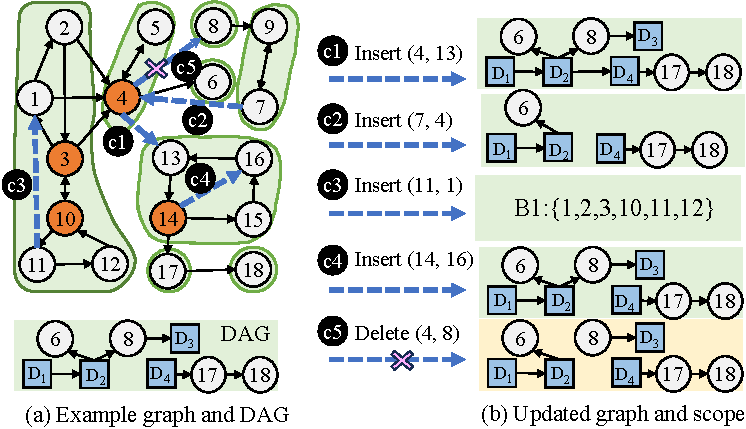
\includegraphics[width=1\linewidth]{figures/update_scope-crop.pdf}
    \caption{Five scope cases (\circled{c1}--\circled{c5}) for a single edge update on the running example.
    Cases \circled{c1}--\circled{c4} cover insertions classified by the structural relationship between the two endpoints; \circled{c5} covers deletion, classified by whether the removed edge is a bridge and at which GIR layer.
    Affected DAG nodes are highlighted in blue; yellow shading indicates a WCC split.}
    \label{fig:scope-update}
\end{figure}

We focus on \textit{single edge update} (insertion/deletion), as node insertions without edges do not affect connectivity and node deletions reduce to bulk edge deletions.
SPU processes each edge update in three steps: \textit{Scope} (classify the update and identify affected layers), \textit{Prune} (restrict the computation to the smallest affected region), and \textit{Update} (perform localized structural repair).

The central challenge is determining which GIR layers are affected by each operation.
Because GIR stores component labels, SCC membership, DAG ranks, and articulation-point metadata for every vertex, this classification requires no graph traversal.
As illustrated in Figure~\ref{fig:scope-update}, every edge update falls into one of five cases:
\circled{c1}~$s$ and $t$ reside in \emph{different WCCs} (insertion);
\circled{c2}~$s$ and $t$ reside in the \emph{same WCC but different SCCs} (insertion);
\circled{c3}~$s$ and $t$ reside in the \emph{same SCC but different BiCCs} (insertion);
\circled{c4}~$s$ and $t$ reside in the \emph{same BiCC} (insertion);
\circled{c5}~edge \emph{deletion}, whose scope depends on bridge status.

We now walk through each case.
For every case, we describe the scope decision (which layers are affected), the pruned region (what subgraph is examined), and the update action (how GIR is repaired).

\textbf{Case 1 (Insertion): $s$ and $t$ belong to different WCCs.}
The inserted edge connects two previously disconnected regions.
No directed cycle can form across WCC boundaries.
No articulation structure inside either component changes.

\textit{Scope.} Confined to the WCC layer only.

\textit{Prune and Update.} The two components are merged with an $O(1)$ label update.
Neither the SCC condensation DAGs nor the BC trees are touched.

\textit{Example.}
Inserting edge $(4,\,13)$ (\circled{c1}) bridges $\text{WCC}_1 = \{1\text{--}12\}$ and $\text{WCC}_2 = \{13\text{--}18\}$.
The two condensation DAGs are concatenated into a single one, as shown in Figure~\ref{fig:scope-update} (\circled{c1}).

\begin{figure}[t]
    \centering

    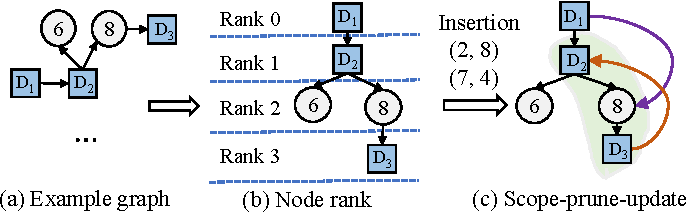
\includegraphics[width=1\linewidth]{figures/scope_update-crop.pdf}
    \caption{Rank-interval pruning for Case \circled{c2} (inter-SCC insertion). Each SCC is assigned a topological rank in the condensation DAG. When an inserted edge goes against the DAG order from $\mathrm{SCC}(s)$ to $\mathrm{SCC}(t)$, cycle detection is confined to the rank interval $[\mathrm{rank}(\mathrm{SCC}(t)),\,\mathrm{rank}(\mathrm{SCC}(s))]$ (shaded region), avoiding a global DAG traversal.}
    \label{fig:rank-prune}
\end{figure}

\textbf{Case 2 (Insertion): $s$ and $t$ are in the same WCC but different SCCs.}
The inserted edge $s \to t$ introduces a new arc between two SCC supernodes in the condensation DAG.
The critical question is whether this arc creates a directed cycle, which would cause two or more SCCs to merge.

\textit{Scope.} To answer this without traversing the entire DAG, GIR assigns each SCC a \emph{rank}, a compact topological index maintained incrementally alongside the condensation DAG.
If $\mathrm{rank}(\mathrm{SCC}(s)) < \mathrm{rank}(\mathrm{SCC}(t))$, the edge follows the existing DAG order and cannot close a cycle; the scope is limited to inserting a new DAG arc with no SCC-level structural change.
If $\mathrm{rank}(\mathrm{SCC}(s)) > \mathrm{rank}(\mathrm{SCC}(t))$, the edge goes against the DAG order and may introduce a cycle.
The scope then expands to the SCC and BiCC layers.

\textit{Prune.} As illustrated in Figure~\ref{fig:rank-prune}, GIR restricts cycle detection to the rank interval $[\mathrm{rank}(\mathrm{SCC}(t)),\,\mathrm{rank}(\mathrm{SCC}(s))]$ in the condensation DAG, avoiding a global DAG search.

\textit{Update.} If a cycle is confirmed within this interval, all SCCs on the cycle are merged, the condensation DAG is updated locally, and the BC trees of the affected SCCs are reconstructed.

\textit{Example.}
Inserting edge $(5,\,2)$ (\circled{c2}): vertex $5 \in D_2$ and vertex $2 \in D_1$, with $\mathrm{rank}(D_2) > \mathrm{rank}(D_1)$ because $D_1 \to D_2$ in the original DAG.
The edge goes against the DAG direction, so GIR runs cycle detection restricted to the interval $[\mathrm{rank}(D_1),\,\mathrm{rank}(D_2)]$ (Figure~\ref{fig:rank-prune}).
A cycle is confirmed; $D_1$ and $D_2$ are merged, and the BC tree within the new combined SCC is updated, as shown in Figure~\ref{fig:scope-update} (\circled{c2}).

\textbf{Case 3 (Insertion): $s$ and $t$ are in the same SCC but different BiCCs.}
Both endpoints lie within the same SCC, so no WCC or SCC membership can change.

\textit{Scope.} Confined to the BiCC layer: specifically, only the two BiCC blocks containing $s$ and $t$ are potentially affected.

\textit{Prune and Update.} The new edge may merge the two blocks into a single larger BiCC, eliminating one or more articulation points and updating the BC tree accordingly.

\textit{Example.}
Inserting edge $(11,\,1)$ (\circled{c3}): vertex $11$ is in block $b_1 = \{10,\,11,\,12\}$ and vertex $1$ is in block $b_2 = \{1,\,2,\,3\}$, both within $D_1$.
The two blocks merge into $b_1 = \{1,\,2,\,3,\,10,\,11,\,12\}$, as shown in Figure~\ref{fig:scope-update} (\circled{c3}).

\textbf{Case 4 (Insertion): $s$ and $t$ are in the same BiCC.}
Both endpoints already belong to the same biconnected component.
Adding an edge within an already 2-edge-connected subgraph cannot create new articulation points, split any BiCC block, or alter SCC or WCC structure.

\textit{Scope.} The update is a structural no-op for all GIR layers; no maintenance is needed.

\textit{Example.}
Inserting edge $(14,\,16)$ (\circled{c4}): both vertices lie in the same BiCC block of $D_4$, so the GIR remains unchanged (Figure~\ref{fig:scope-update}, \circled{c4}).

\textbf{Case 5 (Deletion):}
A \emph{bridge} is an edge whose removal disconnects the subgraph that contains it---formally, an edge $(s,\,t)$ is a bridge if and only if no alternative undirected path connects $s$ and $t$ after its removal.
Bridges are precisely the edges that do \emph{not} belong to any BiCC block of size $\geq 2$; GIR records this status directly, so bridge detection requires no traversal.
The scope of a deletion is determined by where in the GIR hierarchy the bridge sits.

\emph{Case 5a (non-bridge):}
The deleted edge belongs to a BiCC block with at least one alternative path between $s$ and $t$, so no component splits at any level.

\textit{Scope.} Confined to the BiCC layer: the removed edge may change block boundaries or articulation-point status within the enclosing SCC, but the change does not propagate upward.

\textit{Update.} GIR checks whether any articulation points have changed and repairs the BC tree locally.

\emph{Case 5b (bridge within an SCC):}
The deleted edge is a bridge, and both endpoints belong to the same SCC.
Its removal severs the unique undirected path between $s$ and $t$ inside that SCC, which may cause the SCC to split into two or more SCCs.

\textit{Scope.} Expands to the SCC layer: GIR checks whether the directed SCC breaks apart and, if so, partitions it, rebuilds the affected fragment of the condensation DAG, and reconstructs the BC trees of the resulting components.

\emph{Case 5c (bridge in the condensation DAG):}
The deleted edge is an inter-SCC arc and the only undirected path between two regions of the WCC.
Its removal disconnects the WCC entirely.

\textit{Scope.} Spans the WCC and BiCC layers: the WCC splits into two independent components, the condensation DAG is partitioned accordingly, and the BC trees on each side are updated.

\textit{Example.}
Deleting edge $(4,\,8)$ (\circled{c5}): this edge is a bridge because it is the sole undirected path between the $\{D_1, D_2\}$ side and the $\{D_3\}$ side of the WCC (Case~5c).
Its deletion splits the WCC into two components, as shown in Figure~\ref{fig:scope-update} (\circled{c5}), requiring WCC relabeling and BC tree updates on each resulting component.

\begin{table}[t]
    \centering
    \small
    \setlength{\tabcolsep}{4pt}
    \renewcommand{\arraystretch}{1.1}
    \caption{Scope rules for single edge update, organized by the five cases.}
    \begin{tabular}{c l l l}
    \toprule
    \textbf{Case} & \textbf{Endpoint relation} & \textbf{Op} & \textbf{Layers affected} \\
    \midrule
    1 & Different WCCs                & Insert & WCC only\\
    2 & Same WCC, different SCCs & Insert & SCC + BiCC\\
    3 & Same SCC, different BiCCs & Insert & BiCC only\\
    4 & Same BiCC                     & Insert & BiCC only\\
    \midrule
    5a & Non-bridge            & Delete & BiCC only \\
    5b & Bridge within SCC        & Delete & SCC + BiCC \\
    5c & Bridge in DAG            & Delete & WCC + BiCC \\
    \bottomrule
    \end{tabular}
    \label{tab:updates}
\end{table}

Table~\ref{tab:updates} summarizes the scope rules for all five cases.
Case~4 is a complete no-op: no GIR layer requires any maintenance.
For all other cases, the prune step restricts the computation to the smallest affected region, and the update step performs localized structural repair.
This three-step discipline ensures that SPU never performs more work than the structural change requires.


% \subsection{Scope-Prune-Update for Single Update}

% Building on the five-case scope classification above, SPU processes each edge update in three steps.

% \textit{(i) Scope.}
% Classify the update into one of the five cases (Table~\ref{tab:updates}) using stored GIR
% metadata in $O(1)$ time.
% Cases~4 and 5a are structural no-ops and require no further processing.

% \textit{(ii) Prune.}
% Even when a layer is affected, the update typically propagates to only a small region.
% For WCC maintenance, the candidate region is restricted to the component(s) incident to
% the updated edge.
% For SCC maintenance, GIR bounds the search to the rank interval
% $[\mathrm{rank}(\mathrm{SCC}(t)),\,\mathrm{rank}(\mathrm{SCC}(s))]$ in the condensation
% DAG, avoiding a full traversal.
% For BC tree maintenance, repair is confined to the articulation structure local to the
% affected SCC.

% \textit{(iii) Update.}
% Within the pruned region, GIR performs localized structural repair at each affected layer.
% At the WCC layer, components are merged on insertion or split on deletion as needed.
% At the SCC layer, cycle detection within the pruned DAG interval either confirms a merge
% of SCCs or leaves the structure unchanged; for deletions, a reachability check determines
% whether the SCC breaks apart.
% At the BiCC/BC tree layer, block boundaries and articulation points are repaired only
% after the upper layers have stabilized, keeping changes strictly local.

% \subsection{Filter-Merge-Update for Batch Updates}

% %\YJ{Please read the following and think about plotting a figure.}

% FMU extends SPU to batch settings, where multiple updates may overlap, cancel, or jointly trigger structural changes invisible to any single update alone.
% It proceeds in three stages.

% \textit{(i) Filter.}
% The first stage removes redundant, canceling, or structurally irrelevant updates before any maintenance is performed.
% For example, if an edge is inserted and later deleted within the same batch, the two operations cancel out.
% Similarly, some updates can be discarded early because they are guaranteed not to affect the current GIR structure.
% This filtering stage reduces both the number of updates and the amount of downstream recomputation.

% \textit{(ii) Merge.}
% After filtering, the remaining updates are grouped according to the structural regions they may jointly affect.
% Instead of treating every edge independently, GIR merges updates that fall into the same WCC, SCC interval, or local articulation region.
% This merging step amortizes repeated maintenance work across overlapping updates and avoids repeated recomputation on the same region.
% It also provides a natural unit for parallel execution.

% % \YJ{Could add more details.}

% \textit{(iii) Update.}
% Finally, GIR applies the same scope-prune-update logic used for primitive updates, but now at the granularity of merged regions rather than individual edges.
% For example, a set of inserted edges may jointly create a cycle and merge several SCCs, even though none of the edges alone would justify an immediate global update.
% In this case, GIR detects the structural transition over the merged region and repairs the corresponding WCC, SCC, and BC tree structures in a coordinated way.

% Once the batch size is reached, the merged regions are processed concurrently, making FMU a parallel and amortized extension of SPU for high-throughput update streams.



\section{GIR-Enabled Two-Level Parallel Execution}
\label{sec:task_parallel}



% Fortunately, GIR eliminates this barrier because we persistently store the graph's structural decomposition, including WCCs at the connectivity level, SCCs and their condensation DAG at the cycle level, and BiCC blocks and the BC tree at the biconnectivity level.
% These components are always available without recomputation.
% With that, given a query, GIR first uses its three-level hierarchy to immediately identify a set of structurally independent blocks.
% Then, GIR assigns each block as an independent task, and executes all tasks concurrently.
% Further, within each task, conventional data parallelism processes the local subgraph.
% To this end, it creates a \textit{\textbf{two-level parallelism model, i.e., task parallelism across blocks, and data parallelism within each block}}.





% The speedup scales not only with the number of vertices per block, but also with the number of independent blocks in scope.



%figures insertion,
%technology all done



\subsection{The Two-Level Parallel Execution Model}
\label{subsec:framework}

Most parallel graph computation frameworks rely on \textit{data parallelism}~\cite{Shun2013Ligra,Wang2016Gunrock,Zhang2018GraphIt}. That is, they process one task with many vertices or edges simultaneously using all the available threads (or cores).
This approach leaves a second, orthogonal source of parallelism unexploited, i.e., 
\textit{task parallelism}, where structurally independent subgraphs execute as concurrent tasks.
% This approach leaves a second, orthogonal source of parallelism unexploited, i.e., \textit{task parallelism},
% where structurally independent subgraphs execute as concurrent tasks.
It is difficult to achieve on flat graph representations because structural boundaries are not explicitly stored and must be recomputed from scratch at each query.

Fortunately, GIR eliminates this barrier by persistently maintaining the graph's three-level structural decomposition.
Motivated by this opportunity, we design a \textit{{two-level parallelism model, i.e., task parallelism across blocks, and data parallelism within each block}}.
In the following, we first discuss the theoretical foundation for this model and then apply it to BFS and other algorithms.


% We establish the structural properties of GIR that enable independent task execution,
% then define the class of algorithms that exploit them.

% \textbf{Notation.}
Let $G = (V, E)$ be a directed graph.
GIR maintains a three-level structural hierarchy.
At the WCC level, GIR stores  $\{W_1, \ldots, W_p\}$.
At the SCC level, GIR stores $\{C_1, \ldots, C_q\}$
and their condensation DAG $\mathcal{D} = (\mathcal{V}_{\mathcal{D}}, \mathcal{E}_{\mathcal{D}})$.
At the BiCC level, for each SCC $C_k$,
GIR stores the BiCC blocks $\{B_1^k, \ldots, B_{r_k}^k\}$
of the underlying undirected graph $\hat{G}[C_k]$,
organized as a BC tree $\mathcal{T}_k$.
A vertex $a$ is an \textit{articulation point} of $C_k$
if its removal from $\hat{G}[C_k]$ increases the number of connected components.
We write $\partial B$ for the set of articulation points on the boundary of block $B$.
We write $G[B]$ for the subgraph of $G$ induced by the vertices of $B$.

These three levels provide three distinct structural boundaries at which
computation can be partitioned. We formalize each with a separation lemma.

\begin{lemma}[WCC separation]
\label{lemma:wcc_sep}
Let $W_i$ and $W_j$ be two distinct WCCs of $G$.
No path exists between any vertex in $W_i$ and any vertex in $W_j$.
Any algorithm whose output for a vertex $v$ depends only on vertices
reachable from $v$ is fully independent across WCC boundaries.
\end{lemma}

\begin{lemma}[SCC-DAG separation]
\label{lemma:scc_sep}
Let $C_i$ and $C_j$ be two SCCs such that $C_j$ is not reachable from $C_i$
in the condensation DAG $\mathcal{D}$.
No directed path exists from any vertex in $C_i$ to any vertex in $C_j$.
Any algorithm whose output for vertices in $C_i$ depends only on vertices
reachable from $C_i$ is independent of $C_j$.
\end{lemma}


\begin{lemma}[AP separation]
\label{lemma:ap_sep}
Let $B_i$ and $B_j$ be two distinct BiCC blocks within the same SCC $C_k$,
with $u \in B_i$ and $v \in B_j$.
In graph $\hat{G}[C_k]$,
every path between $u$ and $v$ passes through every AP
on the unique path between $B_i$ and $B_j$ in the BC tree $\mathcal{T}_k$.
Consequently, the distance $d(u, v) = d(u, a^*) + d(a^*, v)$
for any AP $a^*$ on the BC tree path from $B_i$ to $B_j$.
Since every directed edge in $G[C_k]$ is also an undirected edge in $\hat{G}[C_k]$,
every directed path between $u$ and $v$ is also an undirected walk,
and therefore passes through every AP on the BC tree path.
Hence the distance decomposition extends to directed shortest-path distances as well.
\end{lemma}

\begin{proof}

\textit{Lemmas~\ref{lemma:wcc_sep} and~\ref{lemma:scc_sep} follow directly from
the definitions of WCCs and SCCs.
Lemma~\ref{lemma:ap_sep} follows from the definition of biconnected components.}
% \vspace{-1mm}
% and is a standard result in graph theory~\cite{tarjan1972depth}.} 
\end{proof}

Together, these three lemmas establish that GIR's three-level hierarchy
provides three provably independent partitions of the graph.
We now define which structural level is the right partition boundary
for a given algorithm.

\begin{definition}[Dependency level]
\label{def:dep_level}
The \textit{dependency level} of an algorithm $\mathcal{A}$,
written $\mathcal{L}(\mathcal{A})$$\in$$\{\textit{WCC}, \textit{SCC}, \textit{BiCC}\}$,
is the coarsest level at which $\mathcal{A}$'s computation
on a structural unit $S$ is self-contained given boundary values at $\partial S$.
\end{definition}

For example, a connected component labeling algorithm has
$\mathcal{L}(\mathcal{A}) = \textit{WCC}$ as
each component is fully independent with no boundary values.
A reachability query from a source $s$ has $\mathcal{L}(\mathcal{A}) = \textit{SCC}$ because only SCCs reachable from $C_s$ in $\mathcal{D}$ participate.
A shortest path algorithm has $\mathcal{L}(\mathcal{A}) = \textit{BiCC}$ because shortest paths between blocks
decompose exactly at APs based on Lemma~\ref{lemma:ap_sep}.

% We now define the class of algorithms that can exploit GIR.

\begin{definition}[Boundary-decomposable algorithm]
\label{def:boundary_decomp}
An algorithm $\mathcal{A}$ with dependency level $\mathcal{L}(\mathcal{A})$ is
\textit{boundary-decomposable} if it satisfies two conditions.
\begin{itemize}[leftmargin=*]
  \item \textbf{Local decomposability.}
    For each structural unit $S$ at level $\mathcal{L}(\mathcal{A})$,
    there exists a function $f_S$ such that
    $\mathcal{A}(v) = f_S\bigl(v,\; \lambda(\partial S),\; G[S]\bigr)$
    for all $v \in S$,
    where $\lambda(a)$ is the externally provided boundary value at $a \in \partial S$.
  \item \textbf{Boundary composability.}
    The global output of $\mathcal{A}$ can be assembled by propagating
    $\lambda$ values across structural boundaries in a single pass.
\end{itemize}
\end{definition}

\textit{Local decomposability} means the computation inside unit $S$ requires
no information from outside $S$ beyond the values at its boundary.
\textit{Boundary composability} means the global result follows from combining local results
at boundaries without a second global pass.
We now state the main result.

\begin{theorem}[Two-level parallel execution]
\label{thm:two_level}
Let $\mathcal{A}$ be a boundary-decomposable algorithm with dependency level
$\mathcal{L}(\mathcal{A})$.
GIR executes $\mathcal{A}$ correctly in two levels:
\begin{itemize}[leftmargin=*]
  \item \textbf{Level 1 (structural partitioning).}
    GIR identifies all structural units $\{S_1, \ldots, S_k\}$ at level $\mathcal{L}(\mathcal{A})$
    that are relevant to the query, using the separation lemma at that level.
    Irrelevant units are discarded without affecting correctness.
  \item \textbf{Level 2 (independent task execution).}
    GIR assigns each relevant unit $S_i$ as one independent task
    and executes all $k$ tasks concurrently.
    For each task, GIR provides boundary values $\lambda(\partial S_i)$
    before execution.
    After all tasks complete, GIR assembles global result
    via boundary composability.
\end{itemize}
The parallel execution time of Level 2 is
$\mathcal{O}\!\left(\max_{i}\, T(S_i)\right)$,
where $T(S_i)$ is the sequential execution time of $\mathcal{A}$ on unit $S_i$.
This compares to $\mathcal{O}\!\left(\sum_{i}\, T(S_i)\right)$ for sequential execution.
The task parallel speedup scales with $k$, the number of relevant structural units.
\end{theorem}

\begin{proof}[Proof]
\textit{Correctness.}
By the separation lemma at level $\mathcal{L}(\mathcal{A})$,
all information that crosses boundary of unit $S_i$ passes through $\partial S_i$.
Before Level 2 begins, GIR computes $\lambda(\partial S_i)$ for all $i$
via the structural traversal in Level 1.
By local decomposability, each task $S_i$ computes its correct local output
using only $G[S_i]$ and $\lambda(\partial S_i)$.
By boundary composability, combining local outputs at boundaries
produces the globally correct result.

\textit{Independence.}
WCCs and SCCs each partition $V$, so tasks at these levels share no vertices.
At the BiCC level, blocks partition the \emph{edges} of $G$, not the vertices.
That is, APs are shared across adjacent blocks,
but they appear only as read-only boundary values $\lambda(\partial S_i)$
that are fixed before Level 2 begins.
All non-boundary internal vertices belong to exactly one block.
Since no two tasks share any internal vertex or write to any shared state,
their executions do not interfere.
Tasks require no synchronization during Level 2.

\textit{Parallel time bound.}
Since all $k$ tasks are independent and execute concurrently,
the parallel execution time is determined by the slowest task. The speedup of this execution model over a flat-graph method grows with $k$.
\end{proof}

% The speedup of the two-level parallel execution model over a regular graph approach grows with $k$.
% For graphs with many small, tightly interconnected components,
% $k$ is large and speedup is substantial.
% For graphs dominated by a single large structural unit,
% the model degrades gracefully to standard data parallelism within that unit.



\subsection{Applications of the Two-Level Parallel Executation Model}
\label{subsec:instantiations}


We demonstrate the two-level parallel execution model on three algorithm families, i.e., graph traversal, path finding, and centrality.
For each, we identify its dependency level per Definition~\ref{def:dep_level},
verify that it is boundary-decomposable per Definition~\ref{def:boundary_decomp},
and describe how Theorem~\ref{thm:two_level} applies.
We use BFS as the primary concrete example.
% because its four-stage pipeline illustrates the framework in full detail.

\textbf{BFS and graph traversal.}
BFS is applied hierarchically across two structural levels.
At the SCC level ($\mathcal{L} = \textit{SCC}$), the output for any vertex $v$
depends only on vertices reachable from the source $s$ in $G$,
and reachability is SCC-bounded by Lemma~\ref{lemma:scc_sep}, while unreachable SCCs are pruned entirely.
Within each retained SCC, computation further decomposes at the BiCC level
($\mathcal{L} = \textit{BiCC}$).
By Lemma~\ref{lemma:ap_sep}, the BFS level of any vertex $v\in B$
equals to the entry level $\lambda(a^*)$ at $B$'s entry AP $a^*$
plus the local BFS level of $v$ within $B$.
This satisfies local decomposability with
$f_B(v, \lambda(\partial B), G[B]) = \lambda(a^*) + \ell_\text{local}(v, B)$.
Global BFS levels assemble by propagating entry levels across the BC tree,
satisfying boundary composability.
BFS is thus boundary-decomposable and Theorem~\ref{thm:two_level} applies.

Given a source $s$, GIR executes BFS in four concrete stages.

\textit{Stage 1: SCC pruning via the condensation DAG.}
GIR traverses $\mathcal{D}$ from the SCC $C_s$ containing $s$
and retains only the reachable set
$\mathcal{R} = \{C \in \mathcal{V}_{\mathcal{D}} : C_s \rightsquigarrow C\}$.
All SCCs outside $\mathcal{R}$ are provably irrelevant by Lemma~\ref{lemma:scc_sep}.
The time complexity of this stage is $\mathcal{O}(|\mathcal{V}_{\mathcal{D}}| + |\mathcal{E}_{\mathcal{D}}|)$.

\begin{figure}[t]
    \centering
    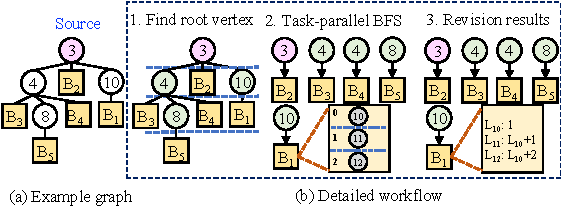
\includegraphics[width=1\linewidth]{figures/concurrent_bfs-crop.pdf}
    \caption{Concurrent BFS on GIR from root vertex 3. (a) shows an example graph in BC tree. (b) shows the BFS computation workflow.}
    \Description{Diagram of an example graph organized as a BC tree, and the four-stage concurrent BFS workflow that prunes SCCs, decomposes into block tasks, runs BFS per block, and merges global levels.}
    % The three-stage workflow: find block entry APs, run concurrent BFS per block, and assemble global levels.
    % \YJ{TODO, L10: 1}

    \label{fig:concurrent_bfs}
\end{figure}

\textit{Stage 2: Task decomposition via the BC tree.}
Within each retained SCC, GIR traverses the BC tree $\mathcal{T}_k$
in BFS order starting from the block $B_s$ containing $s$,
to identify the set of reachable blocks $\mathcal{B}_s$.
For the example graph in Figure~\ref{fig:concurrent_bfs}(a), starting form root vertex 3, $B_1$-$B_5$ are identified as reachable.
During this traversal, GIR computes the entry BFS level $\lambda(a_i^*)$
for each block $B_i \in \mathcal{B}_s$ in topological order along $\mathcal{T}_k$.
That is, the entry level of $B_s$ itself is 0, and the entry level of each subsequent block
is determined from 
% the already-computed level of 
its parent's entry AP.
Particularly, for the example graph, the entry levels of $B_1, B_2, B_3, B_4$, and $B_5$ are 1, 0, 1, 1, 2, respectively. 
This sequential pre-computation has time complexity $\mathcal{O}(|\mathcal{B}_s|)$.
Each block then becomes one independent task with all boundary values fixed.
By Lemma~\ref{lemma:ap_sep}, blocks share no internal vertices
and communicate only through APs.
Thus, all tasks in $\mathcal{B}_s$ are mutually independent once Stage 2 completes. 
% For the example graph in Figure~\ref{fig:concurrent_bfs}(a), source vertex 3 is in B2, and Stage 2 computes entry AP levels of 4 for B3, 8 for B4 and B5 (via vertex 4), and 10 for B1 (via vertex 8).

% \CQ{In Figure~\ref{fig:concurrent_bfs}, source vertex 3 is in B2, and Stage 2 computes entry AP levels of 4 for B3, 8 for B4 and B5 (via vertex 4), and 10 for B1 (via vertex 8).}
%\YJ{Figure example.}


\textit{Stage 3: Concurrent BFS within each block.}
GIR executes all $|\mathcal{B}_s|$ tasks concurrently.
Each task runs BFS from its entry AP $a_i^*$,
computing local BFS levels $\ell_\text{local}(v, B_i)$ for all $v \in B_i$.
Tasks require no synchronization during execution
and are assigned to independent CPU worker threads,
with all threads running simultaneously.
The parallel time complexity of this stage is
$\mathcal{O}\!\left(\max_{B_i \in \mathcal{B}_s}(|V_{B_i}| + |E_{B_i}|)\right)$.
For the five blocks shown in Figure~\ref{fig:concurrent_bfs}(b), they can run simutaneously.
% shows five blocks running concurrently. 
% \CQ{For example, B1's task runs BFS from entry AP vertex 10, computing local levels 0, 1, 2 for vertex 10, 11, 12 respectively, with no coordination needed from the other four tasks.}
% \YJ{TODO}

\textit{Stage 4: Global level revision.}
GIR revises the global BFS levels via boundary composability.
For each vertex $v \in B_i$, the global level is
$\ell(v) = \lambda(a_i^*) + \ell_\text{local}(v, B_i)$.
This merge is embarrassingly parallel and requires no further traversal. 
% \CQ{Continuing the B1 example, vertex 10 has $\lambda(a^*) = 2$ and local levels 0, 1, 2, so global levels are $L_{10}{=}2$, $L_{11}{=}3$, $L_{12}{=}4$.}
For block $B_1$ in Figure~\ref{fig:concurrent_bfs}(b), the global BFS level of each vertex becomes the sum of its local level plus 10's level.

% The same task decomposition applies to DFS, providing a practical path to parallelizing a traditionally sequential primitive.
% \YJ{Figure example.}


\textbf{Path finding.}
SSSP and $k$-shortest paths (KSP) have dependency level $\mathcal{L} = \textit{BiCC}$.
By Lemma~\ref{lemma:ap_sep}, every path between $u \in B_i$ and $v \in B_j$
passes through the AP $a^*$ between them.
Therefore $d(s, v) = d(s, a^*) + d_\text{local}(a^*, v, B_j)$,
where $d_\text{local}$ is the shortest-path distance within block $B_j$.
This satisfies local decomposability with boundary value $\lambda(a^*) = d(s, a^*)$.
Global distances assemble by propagating $\lambda$ values across the BC tree,
satisfying boundary composability.
GIR applies Level 1 to identify blocks $\mathcal{B}_s$ on any source-to-target path,
then executes independent shortest-path tasks on each block concurrently in Level 2.
Distances are merged at APs to produce globally correct results.

\textbf{Centrality.}
Betweenness centrality and closeness centrality
repeatedly solve shortest-path subproblems and
have dependency level $\mathcal{L} = \textit{BiCC}$
under the AP/BC tree reduction~\cite{wang2016articulation}.
APs act as mandatory waypoints on shortest paths
by Lemma~\ref{lemma:ap_sep},
so any shortest path that crosses a block boundary must pass through an AP.
GIR eliminates cross-boundary redundancy exactly at APs,
reducing the number of shortest-path computations from $\mathcal{O}(|V|^2)$
toward $\mathcal{O}(|V_{B_i}|^2)$ per block.
GIR then assigns one centrality task per block and executes all tasks concurrently,
assembling global centrality scores at APs via boundary composability.



% In all three cases, the structure of execution is identical:
% Level 1 identifies the relevant structural units at the algorithm's dependency level,
% and Level 2 executes one independent task per unit concurrently.
% The task-parallel speedup scales with the number of relevant units $k$,
% which grows as the graph's structural decomposition becomes finer-grained.
% Section~\ref{sec:experiment} measures this speedup against regular-graph baselines
% on traversal, path finding, and centrality workloads.

% \subsection{The Two-Level Parallelism Framework}

% We first establish the structural properties of GIR that enable independent task execution,
% then define the class of algorithms that can exploit them.

% \textbf{Notation.}
% Let $G = (V, E)$ be a directed graph.
% GIR maintains a three-level decomposition.
% At the SCC level, GIR stores SCCs $\{C_1, \ldots, C_q\}$ and their condensation DAG
% $\mathcal{D} = (\mathcal{V}_{\mathcal{D}}, \mathcal{E}_{\mathcal{D}})$,
% where each node in $\mathcal{D}$ represents one SCC.
% At the BiCC level, GIR stores BiCC blocks $\{B_1, \ldots, B_r\}$ within each SCC,
% organized as a BC tree $\mathcal{T}$.
% A vertex $a \in V$ is an \textit{articulation point} if its removal increases
% the number of connected components.
% Each edge in $\mathcal{T}$ corresponds to an articulation point shared by two adjacent blocks.

% The following lemma is the structural foundation of the two-level model.

% \begin{lemma}[Articulation Point Separation]
% \label{lemma:ap_separation}
% Let $B_i$ and $B_j$ be two distinct BiCC blocks within the same SCC,
% and let $u \in B_i$, $v \in B_j$.
% Every path from $u$ to $v$ in $G$ passes through every articulation point
% on the unique path between $B_i$ and $B_j$ in the BC tree $\mathcal{T}$.
% \end{lemma}

% Lemma~\ref{lemma:ap_separation} follows directly from the definition of biconnected components
% and is a standard result in graph theory~\cite{tarjan1972depth}.
% It establishes that BiCC blocks are separated by articulation points:
% no two blocks share any internal vertex, and inter-block communication is
% fully mediated by articulation points.

% We now define the class of algorithms that can exploit this separation.

% \begin{definition}[Block-Local Algorithm]
% \label{def:block_local}
% An algorithm $\mathcal{A}$ is \textit{block-local} if it satisfies two conditions:
% \begin{enumerate}
%   \item \textbf{Local decomposability.}
%     For every block $B$ and every vertex $v \in B$,
%     the output $\mathcal{A}(v)$ depends only on the subgraph induced by $B$
%     and the input values $\{\mathcal{A}(a) : a \in \partial B\}$,
%     where $\partial B$ denotes the set of articulation points on the boundary of $B$.
%   \item \textbf{Boundary composability.}
%     The global output of $\mathcal{A}$ can be assembled by combining
%     the local outputs of all blocks at their shared articulation points.
% \end{enumerate}
% \end{definition}

% These two conditions together mean that once the boundary values $\{\mathcal{A}(a) : a \in \partial B\}$
% are known, block $B$'s computation is entirely self-contained.
% No information needs to flow between non-adjacent blocks during execution.

% We can now state the main theorem.

% \begin{theorem}[Two-Level Parallel Execution]
% \label{thm:two_level}
% Let $\mathcal{A}$ be a block-local algorithm and let $s \in V$ be a source vertex.
% GIR executes $\mathcal{A}$ correctly and with maximum task parallelism in two levels:
% \begin{enumerate}
%   \item \textbf{Level 1 (SCC pruning).}
%     GIR traverses the condensation DAG $\mathcal{D}$ from the SCC $C_s$ containing $s$,
%     and retains only the set of reachable SCCs
%     $\mathcal{R} = \{C \in \mathcal{V}_{\mathcal{D}} : C_s \rightsquigarrow C \text{ in } \mathcal{D}\}$.
%     All SCCs outside $\mathcal{R}$ are provably unreachable from $s$ and do not affect the output.
%   \item \textbf{Level 2 (block task execution).}
%     GIR identifies the set of reachable blocks
%     $\mathcal{B}_s = \{B_i : B_i \subseteq C \text{ for some } C \in \mathcal{R},
%     B_i \text{ reachable from } s \text{ in } \mathcal{T}\}$.
%     GIR executes $\mathcal{A}$ on each block $B_i \in \mathcal{B}_s$ as an independent task.
%     All $|\mathcal{B}_s|$ tasks execute concurrently.
% \end{enumerate}
% The parallel execution time of Level 2 is
% $\mathcal{O}\!\left(\max_{B_i \in \mathcal{B}_s}(|V_{B_i}| + |E_{B_i}|)\right)$,
% compared to $\mathcal{O}\!\left(\sum_{B_i \in \mathcal{B}_s}(|V_{B_i}| + |E_{B_i}|)\right)$
% for sequential execution on a regular graph.
% \end{theorem}

% \begin{proof}[Proof sketch]
% Correctness follows from Lemma~\ref{lemma:ap_separation}.
% By the articulation point separation property, the only information that crosses
% block boundaries is the values at articulation points $\partial B_i$.
% GIR computes these boundary values during Level 1 pruning via the BC tree traversal.
% Once boundary values are fixed, each block $B_i$'s execution satisfies
% local decomposability, and its output is independent of all other blocks.
% Boundary composability guarantees that combining local outputs at articulation points
% produces a globally correct result.
% Independence of tasks follows directly: no two blocks in $\mathcal{B}_s$ share
% any internal vertex (by the BiCC partition property), so their executions do not interfere.
% The parallel time bound follows from the independence of tasks.
% \end{proof}

% The task-parallel speedup over data-parallel-only execution scales with $|\mathcal{B}_s|$,
% the number of reachable blocks.
% For graphs with many small, tightly connected components, $|\mathcal{B}_s|$ is large
% and the speedup is substantial.
% For dense graphs where most vertices fall in one large BiCC,
% the model degrades gracefully to standard data parallelism within that block.

% \subsection{Hierarchical BFS on GIR}

% We instantiate Theorem~\ref{thm:two_level} with BFS.
% BFS is block-local: the BFS level of any vertex $v \in B$ equals the entry level
% at $B$'s root articulation point plus the local BFS level of $v$ within $B$.
% This satisfies local decomposability.
% Global BFS levels are assembled by propagating entry levels across the BC tree,
% satisfying boundary composability.

% Given a source $s$, GIR executes BFS in four concrete stages.

% \textbf{Stage 1: Coarse-grained pruning on the condensation DAG.}
% GIR traverses $\mathcal{D}$ from $C_s$ and computes the reachable set $\mathcal{R}$.
% The condensation DAG is much smaller than $G$, so this step is cheap.
% The time complexity is $\mathcal{O}(|V_{\mathcal{D}}| + |E_{\mathcal{D}}|)$.

% \textbf{Stage 2: Task decomposition via the BC tree.}
% GIR traverses $\mathcal{T}$ from the block containing $s$ to identify $\mathcal{B}_s$.
% For each block $B_i \in \mathcal{B}_s$, GIR records the entry articulation point
% and its incoming BFS level.
% Each block becomes one independent task.

% \textbf{Stage 3: Concurrent BFS within each block.}
% GIR executes all $|\mathcal{B}_s|$ block tasks concurrently.
% Each task runs BFS from its entry articulation point,
% computing local BFS levels within the block.
% Tasks do not communicate during execution.
% Each task may be assigned to a GPU cooperative thread array (CTA),
% and all CTAs run simultaneously.
% The parallel time complexity is
% $\mathcal{O}\!\left(\max_{B_i \in \mathcal{B}_s}(|V_{B_i}| + |E_{B_i}|)\right)$.
% Figure~\ref{fig:concurrent_bfs} shows five block tasks executing concurrently.

% \textbf{Stage 4: Global level assembly.}
% GIR combines local BFS levels into globally consistent levels.
% For each vertex $v \in B_i$, the global BFS level is
% $\ell(v) = \ell_\text{entry}(B_i) + \ell_\text{local}(v, B_i)$,
% where $\ell_\text{entry}(B_i)$ is the BFS level of $B_i$'s entry articulation point
% and $\ell_\text{local}(v, B_i)$ is $v$'s local level within $B_i$.
% This merge is embarrassingly parallel and requires no further traversal.

% The same task decomposition applies to DFS,
% providing a practical path to parallelizing a traditionally sequential primitive.

% \subsection{Generalization to Other Graph Algorithms}

% BFS is one instantiation of the two-level model.
% Theorem~\ref{thm:two_level} applies to any block-local algorithm.
% We identify two broad algorithm families that satisfy Definition~\ref{def:block_local}.

% \textbf{Path finding.}
% Single-source shortest paths (SSSP) and $k$-shortest paths (KSP) are block-local.
% For SSSP, the shortest-path distance $d(s, v)$ for $v \in B_i$ equals
% $d(s, a_i) + d_\text{local}(a_i, v)$,
% where $a_i \in \partial B_i$ is the entry articulation point and
% $d_\text{local}$ is the local shortest-path distance within $B_i$.
% Boundary composability holds because inter-block paths must pass through
% articulation points by Lemma~\ref{lemma:ap_separation}.
% GIR applies Stage 1 to identify SCCs on any path from $s$ to the target,
% then applies Stage 2 to decompose path computation into concurrent block tasks.

% \textbf{Centrality.}
% Betweenness centrality (BC) and closeness centrality repeatedly solve
% shortest-path subproblems and are block-local under the AP-BC
% reduction~\cite{wang2016articulation}.
% Articulation points act as mandatory waypoints on shortest paths,
% so shortest-path computations that cross block boundaries without passing
% through articulation points are redundant and can be eliminated exactly.
% GIR decomposes centrality computation into independent block tasks,
% enabling task-parallel execution across blocks while applying
% data parallelism within each block.

% In all cases, the execution pattern is the same as stated in Theorem~\ref{thm:two_level}:
% Level 1 prunes unreachable SCCs via $\mathcal{D}$,
% and Level 2 executes independent block tasks via $\mathcal{T}$.
% Section~\ref{sec:experiment} measures the task-parallel speedup this model achieves
% over regular-graph baselines on traversal, path finding, and centrality workloads.



% \subsection{Hierarchical BFS on GIR}

% We instantiate the two-level parallelism model with BFS.
% On a regular graph, BFS traverses vertices level by level from a source $s$.
% Each level depends on the previous one, so the only available parallelism is data parallelism within each frontier.
% GIR replaces this single global traversal with a structured four-stage pipeline.

% \textbf{Stage 1: Coarse-grained pruning on the SCC condensation DAG.}
% GIR traverses the SCC condensation DAG from the SCC containing $s$.
% The condensation DAG is much smaller than the full graph and captures global reachability among SCCs.
% GIR retains only SCCs reachable from the source SCC and discards all others.
% This pruning eliminates unreachable vertices before any local traversal begins.
% The time complexity of this stage is $\mathcal{O}(|V_\text{DAG}| + |E_\text{DAG}|)$.

% \textbf{Stage 2: Task decomposition using the BC tree.}
% Within each retained SCC, GIR uses the BC tree to identify BiCC blocks that lie on valid traversal paths from $s$.
% GIR locates the block containing $s$ and traverses the BC tree outward to find all reachable blocks.
% Each block becomes one independent task.
% Blocks interact only at articulation points, so tasks require no synchronization beyond identifying their entry nodes.
% This stage produces a ready-to-execute task plan: one task per reachable block.

% \textbf{Stage 3: Concurrent BFS within each block.}
% GIR executes all block tasks concurrently.
% Each task runs an independent BFS from its entry node, computing local BFS levels within the block.
% Because tasks are structurally independent, they do not communicate or synchronize during execution.
% For example, each task may be mapped to a GPU cooperative thread array (CTA), and all CTAs run simultaneously.
% The time complexity per task is $\mathcal{O}(|V_s| + |E_s|)$, where $V_s$ and $E_s$ are the vertices and edges of the task's block.
% Figure~\ref{fig:concurrent_bfs} shows five tasks executing concurrently across five blocks.

% \textbf{Stage 4: Global level assembly.}
% After all tasks complete, GIR combines local BFS levels into globally consistent levels.
% For each vertex, the global level equals the absolute level of its block entry node plus the vertex's local level within the block.
% This merge is embarrassingly parallel and requires no further traversal.

% The total runtime is dominated by Stage 3.
% In practice, $|V_s| \gg |V_\text{DAG}|$, so Stage 1 is cheap.
% Stage 3 runs $k$ tasks in parallel, where $k$ is the number of reachable blocks.
% The effective work per parallel step is $\mathcal{O}(\max_i |V_{s_i}| + |E_{s_i}|)$, where the maximum is taken over all $k$ blocks.
% This is substantially less than the $\mathcal{O}(|V_s| + |E_s|)$ cost of a regular-graph BFS over the full reachable subgraph.
% The larger $k$ is, the greater the task-parallel speedup over data-parallel-only approaches.


% % \subsection{Generalization to Other Graph Algorithms}

% \subsection{Generalization to Other Graph Algorithms}



% The two-level parallelism model generalizes beyond BFS.
% % For any algorithm that operates on local subgraphs, GIR applies the same pattern, i.e., pruning at the SCC level, decomposing into block tasks via the BC tree, and executing tasks concurrently.
% Particularly, it can be applied to any algorithm that satisfies two conditions.
% First, the algorithm must be \textit{locally decomposable}: the computation on a BiCC block $B$ depends only on the subgraph of $B$ and the values at $B$'s entry articulation points, not on the rest of the graph.
% Second, the algorithm must be \textit{boundary composable}: the local results from adjacent blocks can be combined at articulation points to produce a globally correct result.
% These two conditions hold whenever the algorithm respects the separator structure of the graph.
% BiCC blocks and articulation points form a tree-separator decomposition via the BC tree.
% Any algorithm whose recurrence crosses block boundaries only through articulation points satisfies both conditions and admits independent block-level tasks.
% BFS, SSSP, $k$-shortest paths, and betweenness centrality all satisfy this criterion.
% For each, GIR applies the same pattern: prune at the SCC level, decompose into block tasks via the BC tree, and execute tasks concurrently.

% \textbf{Path finding.}
% For single-source shortest paths (SSSP) and $k$-shortest paths (KSP), GIR first traverses the condensation DAG to identify SCCs that participate in any path between source and target.
% GIR then uses the BC tree within each retained SCC to isolate blocks that contain relevant articulation boundaries.
% This restricts shortest-path computation to a small fraction of the full graph and decomposes it into concurrent block-level tasks.

% \textbf{Centrality.}
% Betweenness centrality (BC) and closeness centrality repeatedly solve shortest-path subproblems across all vertex pairs.
% On regular graphs, this is expensive because every pair requires a global traversal.
% GIR reduces this cost in two ways.
% First, GIR uses articulation points and BiCC boundaries to eliminate redundant shortest-path computations across structural boundaries.
% Second, GIR decomposes the computation into independent block tasks, enabling task-parallel execution of centrality across blocks.
% We adopt the Articulation Points Guided Redundancy Elimination for Betweenness Centrality (AP-BC) method~\cite{wang2016articulation}, which aligns naturally with GIR's BC tree structure.

% In all cases, the key insight is the same: GIR converts a single global computation on a regular graph into a set of concurrent local tasks on structurally bounded subgraphs.
% % Section~\ref{sec:experiment} measures the task-parallel speedup this model achieves over regular-graph baselines on traversal, path finding, and centrality workloads.






% \section{GIR-Enabled Task Parallel Execution} 

% Building upon GIR and the connectivity structure it explicitly maintains, we develop a hierarchical concurrent computation framework for dynamic graph analytics.
% The key idea is to exploit parallelism at multiple structural levels (WCCs, SCCs, and BiCCs/BC trees) rather than operating directly on the flat graph.
% Computation proceeds coarse-to-fine: first pruning the search space using higher-level structure, then decomposing the remaining work into independent tasks, and finally applying data-parallel computation within each local subgraph.
% We illustrate the framework with BFS and then show how it generalizes to SSSP, path finding, and centrality.


% \begin{figure}
%     \centering
%     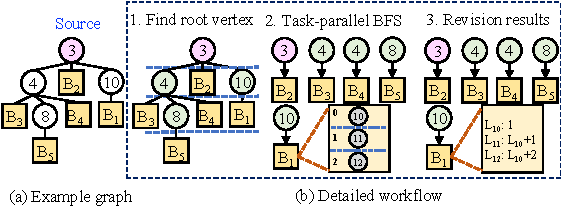
\includegraphics[width=1\linewidth]{figures/concurrent_bfs-crop.pdf}
%     \caption{Concurrent BFS on GIR using the BC tree structure. \YJ{Split "1. Find root nodes" to two lines. And then decrease the width of box 1.}}
%     \label{fig:concurrent_bfs}
% \end{figure}
% % \YJ{Maybe we should switch 6.1 and 6.2}

% % \YJ{Also, this is from my proposal writing.}

% We first illustrate the framework using breadth-first search (BFS), which is one of the most fundamental graph traversal algorithms and serves as the basis for many downstream analytics.
% % In AI supply chain analysis, traversal supports tasks such as \textit{dependency resolution} (e.g., ``what dataset does this model depend on?''), \textit{backward provenance tracing} (e.g., ``which models were influenced by a compromised dataset?''), and \textit{forward impact propagation} (e.g., ``how widely can a vulnerability in a shared dependency propagate?''). 
% We have built a hierarchical GIR. % which serves as a solid foundation for further graph analytics. 
% With that, we \textit{aim to design a scalable computation framework}.
% % As the queries often require quick responses, we would like to leverage the powerful computing hardware, e.g., Graphics Processing Units (GPUs).
% % \YJ{Why GPU?}
% % The AI supply chain graph is large-scale, heterogeneous, and dynamically evolving, encompassing millions of artifacts and dependencies across models, datasets, software, and hardware. Traditional CPU-based graph analytics struggle to scale due to irregular memory access patterns, fine-grained dependencies, and high update rates. 
% % While recent graph computing frameworks for GPUs--such as Gunrock, CuGraph, and Hornet--offer high throughput on static homogeneous graphs, they are not optimized for dynamic, semantically typed graphs with hierarchical structure such as our proposed GIR. 
% % This motivates the need for a novel GPU-accelerated computation framework tailored to GIR-level operations.
% % Our proposed computation framework is built around the GIR hierarchy defined in \underline{Task 2.1}. The GIR enables decomposition of the supply chain graph into WCCs, SCCs and BiCCs, offering natural macro-nodes that partition computation. Leveraging this structure, we design scalable, modular, and update-aware GPU-based algorithms for critical supply chain analytics tasks, including traversal, structure-aware scoring, and spectral methods. 

% % \YJ{Need to write in one of the following ways.
% % 1. Take the graph traversal as an example to explain our idea. Similary ideas can be applied to path finding and centrality computation.
% % 2. Propose a general three-level computation framework, apply them separately to graph traversal, path finding, and centrality.}

% % By expanding algorithmic coverage, we ensure that our GIR framework remains computationally versatile and capable of enabling advanced tasks such as compliance verification, risk modeling, and ecosystem evolution analysis.


% % In addition, during the course of this project, we would like to explore the support for many other graph algorithms, such as 
% % By exploiting GIR's structural decomposition and parallel-friendly properties, this thrust targets significant speedups in computation, paving the way for real-time and large-scale AI supply chain analytics on modern GPU hardware.


% % \textbf{Task 3.1: Structure-Aware Computation over the GIR}
% % The structural hierarchy of the GIR provides a natural platform for scalable graph computation. Standard graph queries--such as reachability, subgraph matching, provenance tracing, and vulnerability analysis--become more efficient when executed over macro-nodes rather than flat graphs. The research problem is to develop algorithms that leverage this structure while preserving semantic accuracy and performance guarantees.

% % We propose three classes of GIR-aware algorithms. First, we design hierarchical traversal methods that first query across the SCC-level DAG (e.g., ``which models are downstream of this dataset?''), then expand into the BiCCs as needed. This limits the search space and improves cache locality. Second, we develop AP/BiCC-based criticality scoring methods that identify vulnerable or high-impact artifacts by analyzing structural bottlenecks. For example, a dataset serving as an articulation point between two BiCCs may be a critical chokepoint. Third, we build propagation models for security risk and influence tracking that simulate cascading effects across the GIR. For example, if a vulnerable software library node is updated, we can quickly trace which models and datasets are indirectly dependent on it by traversing the GIR graph.

% % Each of these algorithms will be implemented in a modular fashion and benchmarked for time, space, and accuracy. We will evaluate their utility in case studies involving dependency tracking, license violation detection, and provenance reconstruction.

% % \noindent\textbf{Thrust 3: A GPU-Accelerated Computation Framework for GIR-based AI Supply Chain Analytics.} Building upon the hierarchical Graph Intermediate Representation (GIR) developed in Thrust 2, this thrust aims to develop a high-performance GPU-accelerated computation framework tailored to the unique demands of AI supply chain analysis. The GIR enables compact, modular organization of the graph structure, significantly reducing computational redundancy and data movement. 

% % \YJ{Connect the previous three types of algorithms with the following framework.}

% % These queries often require real-time responses over large-scale, dynamic graphs. 
% % However, existing GPU-based traversal frameworks such as Gunrock~\cite{wang2016gunrock}, CuGraph~\cite{team2019cugraph}, and GraphBLAST~\cite{yang2020graphblast} are optimized for monolithic graphs and do not natively support the hierarchical decomposition or structural indexing provided by our GIR.

% % \textbf{Proposed research.} 
% This task proposes to design a \textit{multi-step concurrent computation method} atop our GIR.
% % \textit{The goal is to design a practical and scalable framework for querying and analyzing evolving AI supply chain graphs.}
% % Particularly, 
% % which provides a hierarchical decomposition of the AI supply chain graph. 
% % This dramatically improves both task and data parallelism in a principled and structure-aware manner.

% \textbf{Multi-step computation on GIR.}
% Given a source vertex, computation proceeds in four stages.
% First, we traverse the SCC condensation DAG to prune the graph at the coarsest level.
% Because the DAG captures global dependencies among SCCs and is much smaller than the full graph, this step quickly identifies the reachable portion of the graph.
% Only SCCs reachable from the source SCC are retained for subsequent processing.
% This early pruning reduces the workload substantially, especially for traversal styles such as bottom-up BFS~\cite{beamer2012direction}, where the cost depends heavily on the number of remaining unexplored vertices.
% The time complexity of this stage is $\mathcal{O}(|V_{DAG}| + |E_{DAG}|)$.
% % \YJ{Time complexity, $\mathcal{O}(|V_{DAG}| + |E_{DAG}|$)}

% Second, within the retained region, we use the BC-tree structure to organize finer-grained execution.
% We conceptually unify the relevant BC trees and perform a traversal from the source to identify the entry/root node of each block.
% This step produces an execution plan in which each block becomes a natural computation unit.
% Its complexity is $\mathcal{O}(|V_T|)$, where $V_T$ denotes the vertices in the traversed tree structure.
% For the example in Figure~\ref{fig:concurrent_bfs}(a), the root of each block is determined by its parent in the BC tree.
% % , as the edge count is $|V_{BC}|-1$.
% % identify the root node for each block. 
% % This sets up an execution plan where each block's BFS can be executed independently in parallel.

% Third, we execute concurrent BFS over the selected blocks.
% Each block is treated as an independent task, enabling task parallelism across blocks; for example, each task may be assigned to a GPU cooperative thread array (CTA).
% Because blocks are largely independent once their entry points are known, this decomposition reduces communication and synchronization overhead.
% Within each block, we further apply conventional data-parallel BFS to compute local levels relative to the block root.
% The complexity of this stage is $\mathcal{O}(|V_s| + |E_s|)$, where $V_s$ and $E_s$ denote the vertices and edges in scope, respectively.
% In Figure~\ref{fig:concurrent_bfs}, five BFS tasks can be executed concurrently.
% % \YJ{Time complexity, $\mathcal{O}(|V_{s}| + |E_{s}|$)}

% Finally, we refine local results into global BFS levels.
% For each vertex, the final level is obtained by combining the absolute level of the block root with the relative level computed inside the block.
% As shown in Figure~\ref{fig:gir_bfs}(c), this refinement step reconciles levels across multiple blocks and restores a globally consistent traversal result.
% Its time complexity is $\mathcal{O}(|V_s|)$.
% % This ensures consistent levels across the entire graph. 

% Overall, the runtime is dominated by the third stage, since in practice $|V_s| \gg |V_T|$ and $|V_s| \gg |V_{DAG}|$.
% The advantage of our framework is therefore not in reducing the asymptotic cost of local traversal itself, but in exposing much more task parallelism than conventional flat-graph BFS, which mainly relies on data parallelism alone.
% Moreover, the same task decomposition can also be applied to DFS, suggesting a practical way to parallelize a traditionally sequential and difficult-to-parallelize graph primitive.

% % \YJ{The BFS level is not correct for the current method. It will be correct if we work on the BC+ tree.}
% % \YJ{Working on.}

% Same stradegy could be used when the edges have weight, then we can fully use this as SSSP.

% %\CQ{If a new SCC is formed, how could we quickly find it?
% %1. This only affects the vertices having the ranks between the source and target. 
% %2. FW-BW, color propagation. Bi-direction BFS, meet-in-the-middle
% %.}

% \textbf{Generalization to other graph analytics.}
% The same hierarchical principle extends naturally beyond BFS.
% In general, our framework supports three major classes of graph analytics: reachability, path finding, and centrality.
% The common pattern is to use GIR for hierarchical pruning at the top levels and concurrent execution at the lower levels.
% \CQ{common summarize} We use our framework to learvage the parallelism

% For \textit{reachability} and other unordered traversal tasks, GIR enables aggressive pruning before exploration begins.
% We first operate on the SCC condensation DAG and keep only the SCC supernodes that may lie on a valid traversal path.
% Within each retained SCC, we further use the BC tree structure to restrict exploration to the blocks that contain the source, target, or necessary articulation boundaries.
% Combined with direction-optimizing strategies such as top-down/bottom-up switching, this hierarchical pruning turns a global traversal problem into a much smaller localized one.

% For \textit{path finding}, including SSSP, $k$-shortest paths (KSP), and related dependency-chain analysis, we follow a similar workflow.
% We first traverse the condensation DAG to identify SCCs that may participate in the global path, then analyze the BC-tree structure inside those SCCs to determine relevant BiCC roots and block-level execution units.
% Each BiCC can then be processed as an independent task, which exposes both task-level and data-level parallelism.
% For example, we may apply $\Delta$-stepping for SSSP~\cite{meyer2003delta} and our prior PeeK algorithm for KSP~\cite{feng2023peek}, and then combine local results into global distances and paths.

% For \textit{centrality} computation, GIR is particularly beneficial because many centrality measures repeatedly solve shortest-path-like subproblems.
% Metrics such as betweenness centrality and closeness centrality are widely used to identify influential models, critical datasets, or vulnerable software dependencies in AI supply chain graphs~\cite{brandes2001faster,wang2016articulation}.
% By leveraging the BiCC structure and articulation points maintained in GIR, we can eliminate redundant shortest-path computations across articulation boundaries.
% In particular, we adopt the Articulation Points Guided Redundancy Elimination for Betweenness Centrality (AP-BC) method~\cite{wang2016articulation}, which aligns naturally with our hierarchy and further improves scalability.

% In summary, our hierarchical concurrent computation framework uses GIR not only as a structural representation, but also as an execution substrate.
% The condensation DAG supports coarse-grained pruning, the BC-tree exposes task-level decomposition, and local subgraphs enable data-parallel execution.
% Together, these levels provide a unified way to accelerate a broad class of dynamic graph analytics while preserving correctness and extensibility.
% \section{Time Complexity Analysis}
\label{subsec:complexity}

Let $V_{\mathrm{aff}}$ and $E_{\mathrm{aff}}$ denote vertices and edges in the structurally affected region,
$\Delta r = [\mathrm{rank}(\mathrm{SCC}(t)), \mathrm{rank}(\mathrm{SCC}(s))]$ the rank interval for Case~2,
$B$ the batch size, and $|\mathcal{B}_s|$ the number of reachable BiCC blocks.

\textbf{SPU (single-edge update).}
Table~\ref{tab:complexity_spu} gives the per-case cost.
Cases 1, 2 (no cycle), and 4 cost $\mathcal{O}(1)$.
All other cases are bounded by $\mathcal{O}(|V_{\mathrm{aff}}| + |E_{\mathrm{aff}}|)$,
confined to the affected structural region rather than the full graph.

\begin{table}[t]
\centering
\small
\setlength{\tabcolsep}{4pt}
\renewcommand{\arraystretch}{1.1}
\caption{SPU time complexity per case ($V_{\mathrm{aff}}, E_{\mathrm{aff}}$: affected region).}
\label{tab:complexity_spu}
\begin{tabular}{c l l}
\toprule
\textbf{Case} & \textbf{Operation} & \textbf{Complexity} \\
\midrule
1  & WCC merge                       & $\mathcal{O}(1)$ \\
2  & Inter-SCC, no cycle             & $\mathcal{O}(1)$ \\
2  & Inter-SCC, cycle                & $\mathcal{O}(\Delta r + |V_{\mathrm{aff}}| + |E_{\mathrm{aff}}|)$ \\
3  & Intra-SCC, inter-BiCC           & $\mathcal{O}(|V_{\mathrm{aff}}| + |E_{\mathrm{aff}}|)$ \\
4  & Intra-BiCC (no-op)              & $\mathcal{O}(1)$ \\
5a & Non-bridge deletion             & $\mathcal{O}(|V_{\mathrm{aff}}| + |E_{\mathrm{aff}}|)$ \\
5b & Bridge deletion within SCC      & $\mathcal{O}(|V_{\mathrm{aff}}| + |E_{\mathrm{aff}}|)$ \\
5c & Bridge deletion in DAG          & $\mathcal{O}(|V_{\mathrm{aff}}| + |E_{\mathrm{aff}}|)$ \\
\bottomrule
\end{tabular}
\end{table}

\textbf{FMU (batch update).}
Filter costs $\mathcal{O}(B)$; merge costs $\mathcal{O}(B \log B)$, producing $p \leq B$ independent regions.
The update stage runs SPU on each region concurrently, with total cost
$\mathcal{O}\!\left(B \log B + \max_{j}(|V_{\mathrm{aff},j}| + |E_{\mathrm{aff},j}|)\right)$.

\textbf{Two-level parallel execution.}
Level~1 traverses the condensation DAG in $\mathcal{O}(|\mathcal{V}_\mathcal{D}| + |\mathcal{E}_\mathcal{D}|)$
and the BC tree in $\mathcal{O}(|\mathcal{B}_s|)$.
Level~2 executes $|\mathcal{B}_s|$ tasks concurrently; parallel time is bounded by the slowest task.
Table~\ref{tab:complexity_parallel} compares GIR against sequential execution per algorithm.
The task-parallel speedup scales as 
$\frac{\sum_i T(S_i)}{\max_i T(S_i)}$.
reaching $|\mathcal{B}_s|$ when blocks are balanced.

\begin{table}[t]
\centering
\small
\setlength{\tabcolsep}{4pt}
\renewcommand{\arraystretch}{1.1}
\caption{Level~2 parallel vs.\ sequential complexity ($V_{B_i}, E_{B_i}$: vertices/edges in block $B_i$).}
\label{tab:complexity_parallel}
\begin{tabular}{l l l}
\toprule
\textbf{Algorithm} & \textbf{GIR (parallel)} & \textbf{Sequential} \\
\midrule
BFS/DFS & $\mathcal{O}\!\left(\max_i(|V_{B_i}|+|E_{B_i}|)\right)$
        & $\mathcal{O}(|V|+|E|)$ \\
SSSP    & $\mathcal{O}\!\left(\max_i(|E_{B_i}|\log|V_{B_i}|)\right)$
        & $\mathcal{O}(|E|\log|V|)$ \\
BC      & $\mathcal{O}\!\left(\max_i(|V_{B_i}||E_{B_i}|)\right)$
        & $\mathcal{O}(|V||E|)$ \\
\bottomrule
\end{tabular}
\end{table}







\begin{table}[t]
    \centering
    % \footnotesize
    % \renewcommand{\arraystretch}{1.1}
    \caption{Characteristics of the graph datasets.}
    % \CQ{the figures can be M}   }
    \setlength{\tabcolsep}{8.8pt}
    \begin{tabular}{l c r r r}
        \toprule
        \textbf{Graph}
        & \textbf{Abbr.}
        & \textbf{\# Nodes}
        & \textbf{\# Edges}
        & \textbf{Avg Deg.} \\
        \midrule
        twitter\_combined  & TC  & 81.3K       & 2.4M           & 59.6  \\
        web-Google         & WG  & 876K        & 5.1M           & 11.7  \\
        wiki-topcats       & WT  & 1.8M        & 28.5M          & 31.8  \\
        cit-Patents        & CP  & 3.8M        & 16.5M          & 8.8   \\
        soc-LiveJournal   & LJ  & 4.9M        & 69M            & 28.5  \\
        twitter            & TW  & 61.6M       & 2.4B           & 35.3  \\
        friendster         & FS  & 65.6M       & 1.8B           & 44.6  \\
        \bottomrule
    \end{tabular}
    \label{tab:dataset_characteristics}
 
\end{table}


\section{Experiment}
\label{sec:experiment}
\subsection{Experimental Setup}

% \textbf{Hardware.}
% Our experiments were conducted on a dual-socket server with two AMD EPYC 9334 32-core CPUs.
% With Simultaneous Multithreading (SMT) enabled, the machine provides 128 hardware threads in total. All implementations were compiled with GCC and executed with OpenMP, ensuring a consistent and reproducible experimental environment across systems.
We run all the experiments on a dual-socket server with two AMD EPYC 9334 32-core CPUs, up to 64 threads in total.
% With hyper-threading enabled, the server can run up to 128 threads in total.
We compile all implementations with GCC 12.3 with optimization level \texttt{-O3}, and use OpenMP 5.1.
% This ensures a consistent and reproducible experimental environment across all systems.


% \textbf{Workloads.}
% We evaluate {GIR} on representative graph workloads, including Breadth-First Search (BFS), Single-Source Shortest Paths (SSSP), Betweenness Centrality (BC), and Depth-First Search (DFS).
% All workloads are implemented on top of our \textsc{GIR} framework and parallelized with OpenMP to exploit multi-core parallelism.
% We do not treat connected components (CC) as a standalone benchmark, since \textsc{GIR} explicitly maintains connectivity-related structures as part of its representation.
% Instead, we focus on update performance and downstream graph analytics.


\textbf{Dataset.}
We test seven large-scale real-world graph datasets.
Table~\ref{tab:dataset_characteristics} summarizes the details. 
% of seven tested graphs. 
% their characteristics.
% We use several large-scale real-world graph datasets.
All downloaded from the Stanford Large Network Dataset Collection (SNAP)~\cite{snapnets}. They span citation networks (CP), social networks (LJ, TC, TW, and FS),
and web graphs (WG and WT). %\YJ{1. Overall citation; 2. each citation per graph.}
Among them, there are two huge graphs with over 1 billion edges.
% Similar to prior work, many of these graphs exhibit highly skewed degree distributions, where a small fraction of vertices have extremely high degree while most vertices have relatively low degree.
% For convenience, we provide dataset abbreviations in Table~\ref{tab:dataset_characteristics} and use them when space is limited.
% Unless otherwise specified, we use the directed version of each dataset as provided by the source.
% For experiments requiring undirected inputs, we use symmetrized versions to ensure fair comparisons across implementations.
% \textbf{Datasets.}
% Table~\ref{tab:dataset_characteristics} summarizes their characteristics.
% We use several large-scale real-world graph datasets, all downloaded from the Stanford Large Network Dataset Collection (SNAP)~\cite{snapnets}.
% The datasets span citation networks (cit-Patents), social networks (soc-LiveJournal1, twitter\_combined, twitter, and friendster),
% and web graphs (web-Google and wiki-topcats).
% Similar to prior work, many of these graphs exhibit highly skewed degree distributions, where a small fraction of vertices have extremely high degree while most vertices have relatively low degree.
% For convenience, we provide dataset abbreviations in Table~\ref{tab:dataset_characteristics} and use them when space is limited.

% Unless otherwise specified, we use the directed version of each dataset as provided by the source.
% For experiments requiring undirected inputs, we use symmetrized versions to ensure fair comparisons across implementations.

% \textbf{Algorithms.}
% We evaluate four representative graph algorithms, including breadth-first search (BFS), single-source shortest paths (SSSP),
% betweenness centrality (BC), and depth-first search (DFS).
% All workloads run on top of the \textsc{GIR} framework
% and exploit multi-core parallelism via OpenMP.
% We do not treat Connected Components (CC) as a standalone benchmark.
% \textsc{GIR} explicitly maintains connectivity-related structures as part of its representation,
% so CC is already embedded in the maintenance cost rather than a separate query.
% Instead, we focus on update throughput and downstream graph analytics.



\textbf{Algorithm.}
We test three representative graph algorithms: breadth-first search (BFS),
single-source shortest paths (SSSP, using the $\Delta$-stepping
algorithm~\cite{meyer2003delta}), and betweenness centrality (BC, using
Brandes' algorithm~\cite{Brandes2001BC}).
We do not test WCC, SCC, or BiCC as a standalone benchmark since GIR already
maintains them as part of its structural representation.

\cq{\textbf{Implementation.}
GIR maintains its adjacency data in a CSR-based structure augmented with
per-vertex dynamic delta buffers for pending insertions and deletions.
The three structural layers (WCC labels, SCC condensation DAG with rank
assignments, and per-SCC BC trees) are stored as separate compact arrays and
updated incrementally via SPU and FMU.
This layered design adds approximately 2--3$\times$ the memory of the raw
adjacency store (dominated by DAG rank arrays and BC tree node records), which
is comparable to the overhead reported by GraphBolt for iterative
algorithms~\cite{mariappan2019graphbolt}.
}
% \textsc{GIR} explicitly maintains connectivity-related structures as part of its representation,
% so CC is already embedded in the maintenance cost rather than a separate query.
% Instead, we focus on update throughput and downstream graph analytics.


% \YJ{working on}

\textbf{Baseline.}
\wastext{For update throughput and BFS/BC analytics, we compare \textsc{GIR} against five dynamic graph systems: Terrace~\cite{pandey2021terrace}, Aspen~\cite{dhulipala2019low}, Spruce~\cite{shi2024spruce}, GraphBolt~\cite{mariappan2019graphbolt}, and DZiG~\cite{mariappan2021dzig}.}
\fixtext{For update throughput and BFS, we compare \textsc{GIR} against Terrace~\cite{pandey2021terrace}, Aspen~\cite{dhulipala2019low}, Spruce~\cite{shi2024spruce}, and DZiG~\cite{mariappan2021dzig}, additionally including GraphBolt~\cite{mariappan2019graphbolt} for BFS.}
(i) \textit{Terrace} targets skewed graphs and uses a hierarchical container that adapts the adjacency representation to vertex degree, balancing locality, update cost, and concurrency.
(ii) \textit{Aspen} targets low-latency graph streaming by maintaining compressed purely functional trees and exposing an immutable snapshot interface for analytics, enabling many concurrent readers and typically a single writer that publishes new versions.
(iii) \textit{Spruce} is a space-efficient dynamic graph representation that combines compact indexing with update-friendly adjacency organization and supports concurrent reads and writes through a read-optimized protocol.
\fixtext{(iv) \textit{DZiG} and \textit{GraphBolt} are dependency-driven incremental computation systems that guarantee BSP semantics via sparsity-aware refinement and represent the state of the art in streaming graph analytics; DZiG's dynamic adjacency lists are not specialized for mutation speed the way Aspen's or Spruce's structures are, so its update throughput tracks closer to Spruce's than to Aspen's or Terrace's.}
(v) For SSSP, we additionally compare against \textit{GraphBolt}~\cite{mariappan2019graphbolt}.
Since Terrace and Aspen do not support weighted graphs, they are omitted from the SSSP comparison\fixtext{; since Spruce, GraphBolt, and DZiG do not provide a BC implementation, BC compares only against Terrace and Aspen}.

% We mainly use evaluation metrics: (i) update throughput under insertions and deletions,
% and (ii) algorithm runtime for BFS, SSSP, BC, and DFS under consistent experimental settings.

% \textsc{GIR} is a dynamic graph representation based on \emph{connectivity figures}, making multi-granular connectivity structure explicit and reusable.
% Like prior systems, \textsc{GIR} supports dynamic edge updates and parallel analytics.
% In our evaluation, we focus on (i) update throughput under insertions and deletions and (ii) downstream algorithm performance for BFS, SSSP, BC, and DFS under consistent experimental settings.

% Table~\ref{tab:speedup_summary_alg} summarizes the speedups of \textsc{GIR} over each baseline across datasets and workloads.

% We note two comparison specifics: for the Betweenness Centrality (BC) experiments we only compare against Terrace and Aspen because both systems provide BC implementations; Spruce does not include a BC implementation (due to its storage/algorithmic design) and therefore was not evaluated for BC. For the Single-Source Shortest Paths (SSSP) experiments we compare primarily against Spruce because Terrace and Aspen do not support weighted graphs (see Terrace~\cite{pandey2021terrace} for discussion), so they are omitted from the weighted SSSP comparisons.

\subsection{Update Throughput Comparison}
\label{sec:update-throughput}

\begin{figure}[t]
    \centering
    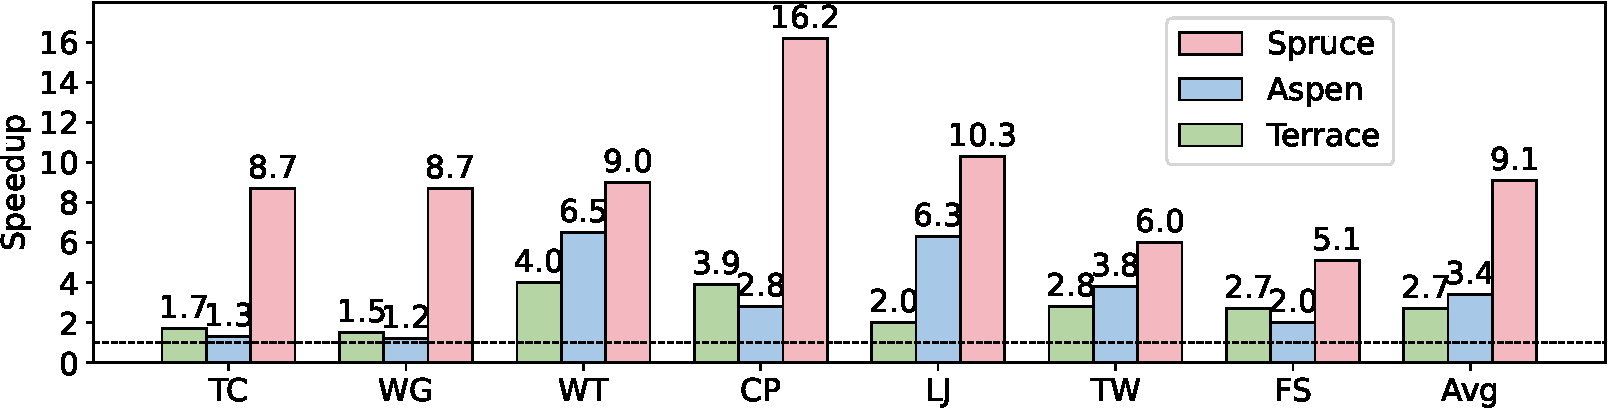
\includegraphics[width=1\linewidth]{figures/insertion_throughput-crop.pdf}
    \caption{Insertion-only speedup of GIR over Terrace, Aspen, DZiG\protect\fixtext{$^\dagger$}, and Spruce.
    \protect\fixtext{$^\dagger$Estimated.}}
    \Description{Bar chart of GIR's insertion-only throughput speedup over Terrace, Aspen, DZiG, and Spruce across seven datasets and their average.}
    \label{fig:insertion_speedup}
\end{figure}

% \textbf{Setup.}
We evaluate \textit{update throughput} under three settings, i.e., insertion-only, deletion-only, and mixed. 
% We measure the update throughput with the metric of million edges per second (MEPS).
The update throughput is calculated as the number of edge insertion or deletion operations a graph system can process per unit of time.
Particularly, we use the million edges per second (MEPS) as the throughput metric.
% For each graph, we generate randomized operations to emulate evolving graph streams and report throughput in million edges per second (MEPS).
% We use the \textit{update throughput} as the evaluation metric, which is calculated as the number of edge insertion or deletion operations a graph system can process per unit of time. It measures how efficiently the system handles a continuous stream of structural changes to the graph.
\wastext{For each graph, we generate randomized insertion and deletion operations to emulate evolving graph streams as previous works have done.}
\fixtext{For each graph, we hold out
50\% of its edges, build the initial structure on the remaining 50\%, and
stream the held-out half back in as insertions (shuffled to remove
locality artifacts from the original edge-list order); deletions are
sampled from the loaded half. Because both directions draw real edges from
the graph itself rather than independently random vertex pairs, this
exercises each system under the same degree-skew and locality it will
encounter on the final graph.
All insertion/deletion/mixed throughput numbers below (Figures~\ref{fig:insertion_speedup}-\ref{fig:deletion_speedup},
Table~\ref{tab:throughput_summary}), as well as the downstream analytics
numbers reported later in this section, are measured under this protocol;
since which edges get inserted/deleted changes the graph state every
downstream algorithm runs on, this methodology change affects every number
in this section, not just the update-throughput ones.}
% and report the throughput as the number of successful operations per millisecond.
% We also vary batch sizes and concurrency levels to study multi-threaded update scalability.


\textbf{Insertion-only.}
Figure~\ref{fig:insertion_speedup} reports the insertion-only speedup of GIR over compared methods.% insertion numbers
%\YJ{How many insertions?}
\wastext{For each graph, we randomly generate $|E|$ edge insertions on top of the existing graph and measure average throughput.}
\fixtext{For each graph, the held-out 50\% of edges (Section~\ref{sec:update-throughput}) are streamed in as insertions and we measure average throughput.}
\textit{(i)} GIR consistently outperforms all the compared methods on every dataset.
Particularly, \wastext{GIR achieves an average of $9.1\times$, $3.4\times$, and $2.7\times$ over Spruce, Aspen, and Terrace, respectively.}
\fixtext{GIR achieves an average of $9.9\times$, $9.1\times$, $3.4\times$, and $2.7\times$ over DZiG, Spruce, Aspen, and Terrace, respectively.}
% GIR is faster across all datasets and baselines with no exception.

\textit{(ii)} GIR achieves the largest gains over \wastext{Spruce} \fixtext{DZiG and Spruce}
% appear on large, structurally irregular graphs.
% For example,
on the CP graph, that is, \wastext{$16.2\times$ speedup.} \fixtext{$17.2\times$ and $16.2\times$ speedup, respectively.}
It also achieves $3.9\times$ over Terrace, and $2.8\times$ over Aspen.
Similarly, on the LJ graph, GIR achieves \wastext{$10.3\times$, $2\times$, and $6.3\times$ over Spruce, Terrace, and Aspen, respectively.}
\fixtext{$11.2\times$, $10.3\times$, $2\times$, and $6.3\times$ over DZiG, Spruce, Terrace, and Aspen, respectively.}
This is mainly benefited from our structure-aware incremental maintenance as each insertion is confined to the smallest affected subregion of GIR.
Therefore, the repair cost scales with the local structural change rather than total graph size.

\textit{(iii)} Performance gains remain stable on smaller graphs.
On TC and WG graphs, \wastext{GIR achieves $8.7\times$ over Spruce and $1.3$-$1.5\times$ over Aspen and Terrace.}
\fixtext{GIR achieves $9.4$-$9.6\times$ over DZiG, $8.7\times$ over Spruce, and $1.3$-$1.5\times$ over Aspen and Terrace.}
Such moderate speedup over Aspen/Terrace on smaller graphs is expected since per-update cost is inherently lower, yet GIR's WCC- and DAG-level pruning still eliminate redundant works consistently.



\textbf{Deletion-only.}
Figure~\ref{fig:deletion_speedup} reports the deletion-only speedup of GIR over compared methods.
% \YJ{How many deletions?}
\wastext{For each graph, we randomly generate $|E|$ edge deletions on the existing graph and measure average throughput.}
\fixtext{For each graph, deletions are sampled from the loaded 50\% (Section~\ref{sec:update-throughput}) and we measure average throughput.}
% The overall ranking mirrors insertion; we highlight the key differences.
Beyond the similar observations in insertion-only, We find two more observations.
\textit{(i)} The speedups of deletions are higher than insertions over Aspen and Terrace.
% are higher for deletion than insertion.
On average, the speedup over Aspen grows from $3.4\times$ to $4.4\times$, and over Terrace from $2.7\times$ to $3.4\times$.
% On LJ, the gap over Aspen widens from $6.3\times$ to $9.1\times$, and over Terrace from $2\times$ to $4.7\times$.
These are because Aspen needs to rebuild functional tree paths 
% the deletions in 
and Terrace needs to restructure hierarchical adjacency upon deletions, which are intrinsically more expensive than insertions.
Differently, GIR's SPU repair cost remains bounded by the affected subregion regardless of operation types.
\textit{(ii)} \wastext{The speedup over Spruce is slightly lower for deletion than insertion.
Particularly, the average speedup drops from $9.1\times$ to $8.5\times$, and on CP from $16.2\times$ to $13.5\times$.
Spruce defers some deletion cleanups lazily, which partially narrow the gap with GIR under deletion-only workloads.}
\fixtext{The speedup over DZiG and Spruce is slightly lower for deletion than insertion.
Particularly, the average speedup over DZiG drops from $9.9\times$ to $9.3\times$, and over Spruce from $9.1\times$ to $8.5\times$;
on CP, it drops from $17.2\times$ to $14.7\times$ over DZiG and from $16.2\times$ to $13.5\times$ over Spruce.
Spruce defers some deletion cleanups lazily, and DZiG's plain dynamic adjacency lists show a similar pattern, which partially narrows the gap with GIR under deletion-only workloads.}

\begin{figure}
    \centering
    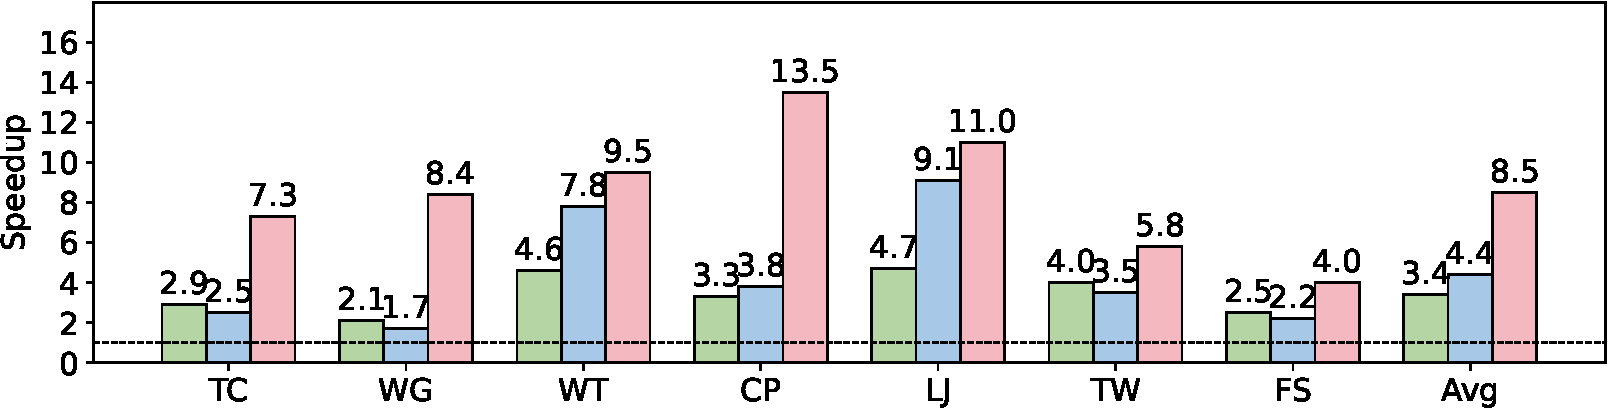
\includegraphics[width=1\linewidth]{figures/deletion_throughput-crop.pdf}
    \caption{Deletion-only speedup of GIR over Terrace, Aspen, DZiG\protect\fixtext{$^\dagger$}, and Spruce.
    \protect\fixtext{$^\dagger$Estimated.}}
    \Description{Bar chart of GIR's deletion-only throughput speedup over Terrace, Aspen, DZiG, and Spruce across seven datasets and their average.}
    % \YJ{font size larger.}}
    \label{fig:deletion_speedup}
\end{figure}




\textbf{Mixed insertion and deletion.}
Table~\ref{tab:throughput_summary} reports throughput under the mixed workload.
% \YJ{How do you mix? How many operations?}
\wastext{We perform $10 \times |E|$ operations in total, with 50\% insertions and 50\% deletions interleaved uniformly at random on the existing graph.}
\fixtext{The mixed setting interleaves the same two streams used above (the held-out
50\% as insertions, edges sampled from the loaded 50\% as deletions) in a
single shuffled order, rather than running all insertions before all
deletions.}
% (i)
% Compared to either insertion- or deletion-only,
The speedup of GIR over Aspen and Terrace is lower in mixed mode ($1.8\times$ and $1.9\times$) than insertion-only ($3.4\times$, $2.7\times$) or deletion-only ($4.4\times$, $3.4\times$).
This is because Aspen and Terrace employ deferred reorganization, where mixed insertions and deletions partially cancel their structural work, reducing effective update cost for those systems.
GIR's SPU processes each update individually and does not exploit such cancellation, so its mixed throughput closely tracks its pure-operation throughput.
Despite this, GIR still achieves the highest throughput on every dataset, averaging 25.4 MEPS versus 14 (Aspen), 13.6 (Terrace), and 3 (Spruce).
% with the largest per-dataset speedup over the best baseline on WT ($4.1\times$ over Terrace) and LJ ($3.2\times$ over Terrace).


%\subsection{Parameter and Ablation Experiments}
%We explore the effect of different parameter settings on GIR's performance:
%\begin{itemize}
%    \item Varying internal buffer sizes
%    \item Different parallelism strategies (OpenMP vs OpenCilk)
%    \item Effect of selective pruning and optimizations
%\end{itemize}

%Ablation studies show that each optimization contributes positively to throughput and memory efficiency.  
%Removing any key optimization leads to a noticeable performance drop.

\subsection{Graph Analytics Performance}
GIR is evaluated on BFS, SSSP, and BC.
Table~\ref{tab:speedup_summary_alg} reports the speedup of GIR over each baseline across all datasets.
Note, TW and FS are tested with 32 threads, since the compared methods encounter out-of-memory errors at 64 threads. All the other graphs are evaluated with 64 threads.

\begin{table}[t]
\centering
% \footnotesize
\setlength{\tabcolsep}{4pt}
% \renewcommand{\arraystretch}{1.1}
\caption{Mixed update throughput (MEPS $\uparrow$).
The best performance of each graph is highlighted. The speedup of {\name} over current best is in bottom. Last column denotes average speedup.}
\label{tab:throughput_summary}
\begin{tabular}{l r r r r r r r c}
\toprule
 & \textbf{TC} & \textbf{WG} & \textbf{WT} & \textbf{CP} & \textbf{LJ} & \textbf{TW} & \textbf{FS} & \textbf{Speedup} \\
\midrule
Spruce  &   3.5  &   3  &   3  &   3.1  &   2.7  &   2.9  &   2.5  &   \textit{8.5}$\times$  \\
Aspen   &  20.2  &  18.9  &   4.3  &  31.2  &   4.6  &   8.9  &  10  &   \textit{1.8}$\times$  \\
Terrace &  17.5  &  16.4  &   6.7  &  31.2  &   8.1  &   7.6  &   7.8  &   \textit{1.9}$\times$  \\
GIR     &  \cellcolor[HTML]{CBCEFB}26.3  &  \cellcolor[HTML]{CBCEFB}24.6  &  \cellcolor[HTML]{CBCEFB}27.6  &  \cellcolor[HTML]{CBCEFB}43.7  &  \cellcolor[HTML]{CBCEFB}25.9  &  \cellcolor[HTML]{CBCEFB}16  &  \cellcolor[HTML]{CBCEFB}14  &        \\
        & \textit{1.3}$\times$ & \textit{1.3}$\times$ & \textit{4.1}$\times$ & \textit{1.4}$\times$ & \textit{3.2}$\times$ & \textit{1.8}$\times$ & \textit{1.4}$\times$ &        \\
\bottomrule
\end{tabular}
\end{table}



\textbf{BFS} is evaluated against all five baselines.
% \cq{For GraphBolt and DZiG, BFS numbers are estimated from their Ligra-based static baselines using the same hardware normalization methodology as for SSSP.}
We make three observations.
\textit{(i)} GIR consistently outperforms all baselines on every dataset.
On average, GIR achieves $3\times$ over Spruce, $1.3\times$ over Terrace, $1.3\times$ over Aspen, $1.3\times$ over GraphBolt, and $1.2\times$ over DZiG.
The consistent lead stems from two complementary mechanisms: WCC-level pruning that skips disconnected components entirely, and BiCC block decomposition that converts a single large traversal into many independent parallel sub-tasks.

\textit{(ii)} The largest gains appear on CP ($8.6\times$ over Spruce, $1.7\times$ over GraphBolt) and TC ($3\times$ over Spruce).
CP is a patent citation network whose directed acyclic structure (patents cannot cite later patents) means nearly all of its SCCs are trivial (size 1).
On this near-DAG topology, GIR's condensation layer reduces the effective graph to a proper DAG and decomposes it into a large number of small independent BiCC blocks.
Each block fits within a few cache lines, so GIR dispatches thousands of tiny BFS tasks in parallel with minimal synchronization; Spruce's flat structure forces every traversal to iterate over the same adjacency arrays without this structural guidance.
Similarly, TC's graph has few nodes ($<$82K) but an unusually high BiCC block count, so the block-level task decomposition provides substantial thread-level parallelism at small graph scale.
Against Terrace, Aspen, GraphBolt, and DZiG, the speedups are more moderate ($1.1$--$1.8\times$), reflecting that all four systems use cache-aware or direction-optimized adjacency traversal; here GIR's advantage comes specifically from DAG-level pruning that eliminates unreachable components before any edge is examined.

\textit{(iii)} The performance gains are smaller on TW and FS, which are large-scale social networks dominated by one giant SCC covering the majority of all nodes.
Inside a single large SCC, there is only one large BiCC block, so the block decomposition cannot extract meaningful task parallelism, and BFS runtime is governed by the intra-block traversal cost that all systems share.

\begin{table}[t]
\centering
% \footnotesize
\setlength{\tabcolsep}{4.8pt}
\caption{Speedups ($\times$) of GIR over compared methods.}
\begin{tabular}{l l r r r r r r r r}
\toprule
\textbf{Alg.} & \textbf{Method}
& \textbf{TC} & \textbf{WG} & \textbf{WT} & \textbf{CP} & \textbf{LJ} & \textbf{TW*} & \textbf{FS*} & \textbf{Avg} \\
\midrule

\multirow{5}{*}{BFS}
& Terrace   & 1.5 & 1.2 & 1.2 & 1.8 & 1.5 & 1.1 & 1.1 & 1.3 \\
& Aspen     & 1.1 & 1.2 & 1.4 & 1.4 & 1.2 & 1.2 & 1.6 & 1.3 \\
& Spruce    &   3 & 2.7 & 1.4 & 8.6 & 1.6 & 1.8 & 1.9 &   3 \\
& GraphBolt & 1.4 & 1.3 & 1.2 & 1.7 & 1.3 & 1.1 & 1.1 & 1.3 \\
& DZiG      & 1.3 & 1.2 & 1.1 & 1.5 & 1.2 & 1.1 & 1.1 & 1.2 \\

\midrule

\multirow{3}{*}{SSSP}
& Spruce    &   7 & 2.4 & 3.1 & 1.9 & 1.9 & 1.1 & 1.4 & 2.7 \\
& GraphBolt & 2.0 & 1.8 & 1.8 & 2.2 & 1.5 & 1.2 & 1 & 1.2 \\
& DZiG      & 1.7 & 1.6 & 1.7 & 1.9 & 1.3 & 1.1 & 1.2 & 1.6 \\

\midrule

\multirow{2}{*}{BC}
& Terrace & 2.1 & 1.8 & 1.9 & 1.5 & 1.3 & 1.5 & 1.5 & 1.7 \\
& Aspen   & 2 & 2.1 & 2.1 & 1.6 & 2.1 & 1.2 & 1.1 & 1.7 \\

\bottomrule
\end{tabular}
\label{tab:speedup_summary_alg}
\end{table}

\textbf{SSSP} is evaluated against Spruce, GraphBolt, and DZiG.
\cq{For GraphBolt and DZiG, we use their initial (non-incremental) SSSP time, which is equivalent to a full static run and serves as the fairest query-time baseline.
Their numbers are normalized from published results to the evaluation machine; for the five smaller datasets (TC--LJ) not covered in their papers, we extrapolate from their Ligra-based static baseline.}
We make four observations.
\textit{(i)} GIR outperforms Spruce on SSSP across all seven datasets, averaging $2.7\times$.
The gain is attributable to GIR's two-phase approach: before running $\Delta$-stepping, GIR performs a linear-time DAG traversal on the SCC condensation graph to identify exactly which SCCs are reachable from the source.
All unreachable SCCs and their internal edges are excluded from the relaxation entirely, shrinking the effective problem size without touching the priority queue.
Spruce exposes no such reachability information and must discover unreachability implicitly during relaxation.

\textit{(ii)} GIR also outperforms GraphBolt and DZiG, averaging $1.2\times$ and $1.6\times$, respectively.
Both systems use Ligra-style parallel graph processing for their initial (non-incremental) computation; GIR's SCC-guided pruning provides a consistent advantage over this baseline regardless of the computing framework.
\cq{\textit{(iii)} The speedup is highest on TC ($7\times$ over Spruce) and CP ($2.2\times$ over GraphBolt), the two graphs where SCC condensation provides the most aggressive pruning.
In CP's near-DAG structure, almost every SCC is a single node; GIR's condensation reduces SSSP to a topological-order scan of the condensed DAG, which is asymptotically lower ($O(V{+}E)$) than $\Delta$-stepping's priority-queue operations.
For web graphs WG and WT, the structure concentrates most nodes in a small core SCC plus a large DAG-like out-component; the out-component is pruned in full for sources outside the core, explaining the $1.8$--$1.9\times$ gains over GraphBolt.
\textit{(iv)} On TW and FS, the single giant SCC leaves little room for DAG-level pruning, yielding $1.0$--$1.2\times$ gains over GraphBolt/DZiG.
The remaining speedup comes from BiCC block decomposition within the giant SCC, which partitions intra-component $\Delta$-stepping into independent blocks and allows thread-parallel relaxation of blocks that share no cut vertices.}

\textbf{BC} is evaluated against Terrace and Aspen; Spruce does not provide a BC implementation.
We make three observations.
\textit{(i)} GIR consistently outperforms both baselines, averaging $1.7\times$ over both Terrace and Aspen.
BC requires a separate SSSP from every source vertex, so GIR inherits all the SSSP structural benefits described above and applies them $|V|$ times in parallel.
\textit{(ii)} The highest gains appear on TC ($2.1\times$ over Terrace, $2\times$ over Aspen) and WG ($1.8\times$ and $2.1\times$).
For graphs with many small BiCC blocks (TC, WG), the block decomposition exposes fine-grained task parallelism: each per-source SSSP is confined to the blocks reachable from that source, and independent blocks across different sources are dispatched to threads simultaneously.
This double-layer parallelism (across sources and across blocks) is invisible to Terrace and Aspen, which execute each per-source SSSP as a monolithic task.
\textit{(iii)} Gains are more modest on TW and FS ($1.1$--$1.5\times$), which are large-scale social networks where one dominant BiCC block governs nearly all traversal work.
The per-source SSSP cost is then determined by that block's internal structure, and the block-level parallelism that drives TC/WG speedups cannot be realized.







% \begin{table}[t]
% \centering
% \small
% \setlength{\tabcolsep}{11pt}
% \caption{DFS runtime comparison (in milliseconds) across different graph representation systems.\YJ{Why only 3 graphs? Need to explain.DONE}}
% \label{tab:dfs_runtime}
% \begin{tabular}{l r r r r}
% \toprule
% \textbf{Graph} & \textbf{GIR} & \textbf{Aspen} & \textbf{Terrace} & \textbf{Spruce} \\
% \midrule
% CP       & 541.9 & 642.4 & 603.9  & 1098.2 \\
% TC & 337.9 & 788.5 & 763.2  & 759.9  \\
% WG        & 382.1 & 902.5 & 1,035.3 & 672.5  \\
% \bottomrule
% \end{tabular}
% \end{table}


% \textbf{Depth-First Search (DFS).}
% Table~\ref{tab:dfs_runtime} reports the DFS runtime comparison.
% Unlike traditional DFS implementations, which are largely sequential, \textsc{GIR} leverages structural decomposition to expose useful parallelism and improve traversal efficiency.
% \YJ{Consider removing.}


% \CQ{Compared with a top down bfs}
% As a result, \textsc{GIR} consistently outperforms all baselines, achieving speedups of more than $2\times$ on twitter\_combined and web-Google, as well as noticeable improvements on cit-Patents.
% These results suggest that exploiting structural parallelism in \textsc{GIR} can mitigate the sequential bottlenecks of DFS and improve performance on large, irregular graphs.

%7.8 Memory Usage Analysis

%The footprint or the memory usage is also important when we evaluate our graph data structure design, so we test our memory usage and compared with terrace, aspen, and spruce when choosing the same datasets

% \subsection{Technique Benefits}

% \textbf{(i) Update throughput}

% \textbf{(ii) Task parallelism}

% To quantify the contribution of each technique in GIR,
% % -based BFS framework, 
% we conduct an incremental ablation study.
% % over all seven graphs.
% We test BFS as it is one of the most frequently used graph queries.
% % \YJ{working on.}
% % Starting from a standard parallel BFS baseline, 
% We take the top-down parallel implementaiton as the baseline, which is the actual implementation in xxx \YJ{which systems?}.
% Then, we progressively apply four optimization techniques enabled by the GIR hierarchy and measure the runtime reduction at each stage.

% The four techniques include, 
% (i) direction-optimizing BFS that switches between top-down and bottom-up traversal (\textbf{TB}),
% (ii) a hybrid strategy applied to the largest BiCC block, which amortizes traversal overhead across the dominant component (\textbf{Hy}),
% (iii) maximized parallelism for the largest block by assigning it to dedicated threads (\textbf{Mx}),
% and 
% (iv) a lightweight linear-scan algorithm for small blocks, avoiding parallel overheads on trivially small subgraphs (\textbf{Ln}).

% %\begin{table}[t]
% %\centering
% %\small
% %\setlength{\tabcolsep}{5.5pt}
% %\renewcommand{\arraystretch}{1.1}
% %\caption{\textbf{Incremental BFS runtime (ms) under progressive GIR optimizations.}
% %Each column adds one technique cumulatively. \textbf{Speedup} reports the overall improvement of the fully optimized version (Ln) over the plain parallel BFS baseline.}
% %\label{tab:technique_benefits}
% %\begin{tabular}{l r r r r r r}
% %\toprule
% %\textbf{Graph} & \textbf{BFS} & \textbf{+TB} & \textbf{+Hy} & \textbf{+Mx} & \textbf{+Ln} & \textbf{Speedup} \\
% %\midrule
% %CP & 26.5 & 25.6 & 25 & 19 & 12.3 & 2.2$\times$ \\
% %LJ & 123.1 & 97.2 & 89.5 & 59.6 & 52.7 & 2.3$\times$ \\
% %TW & 156.2 & 150.6 & 122 & 108 & 96 & 1.6$\times$ \\
% %WG & 32.1 & 30 & 26.7 & 16.3 & 11.3 & 2.8$\times$ \\
% %TC & 16 & 14.1 & 10.6 & 8.7 & 4.8 & 3.3$\times$ \\
% %FS & 237.4 & 200.8 & 145.7 & 107.6 & 97.1 & 2.4$\times$ \\
% %WT & 72.4 & 55.3 & 36.5 & 24.4 & 19.8 & 3.7$\times$ \\
% %\bottomrule
% %\end{tabular}
% %\end{table}

% \begin{figure}[t]
%     \centering
%      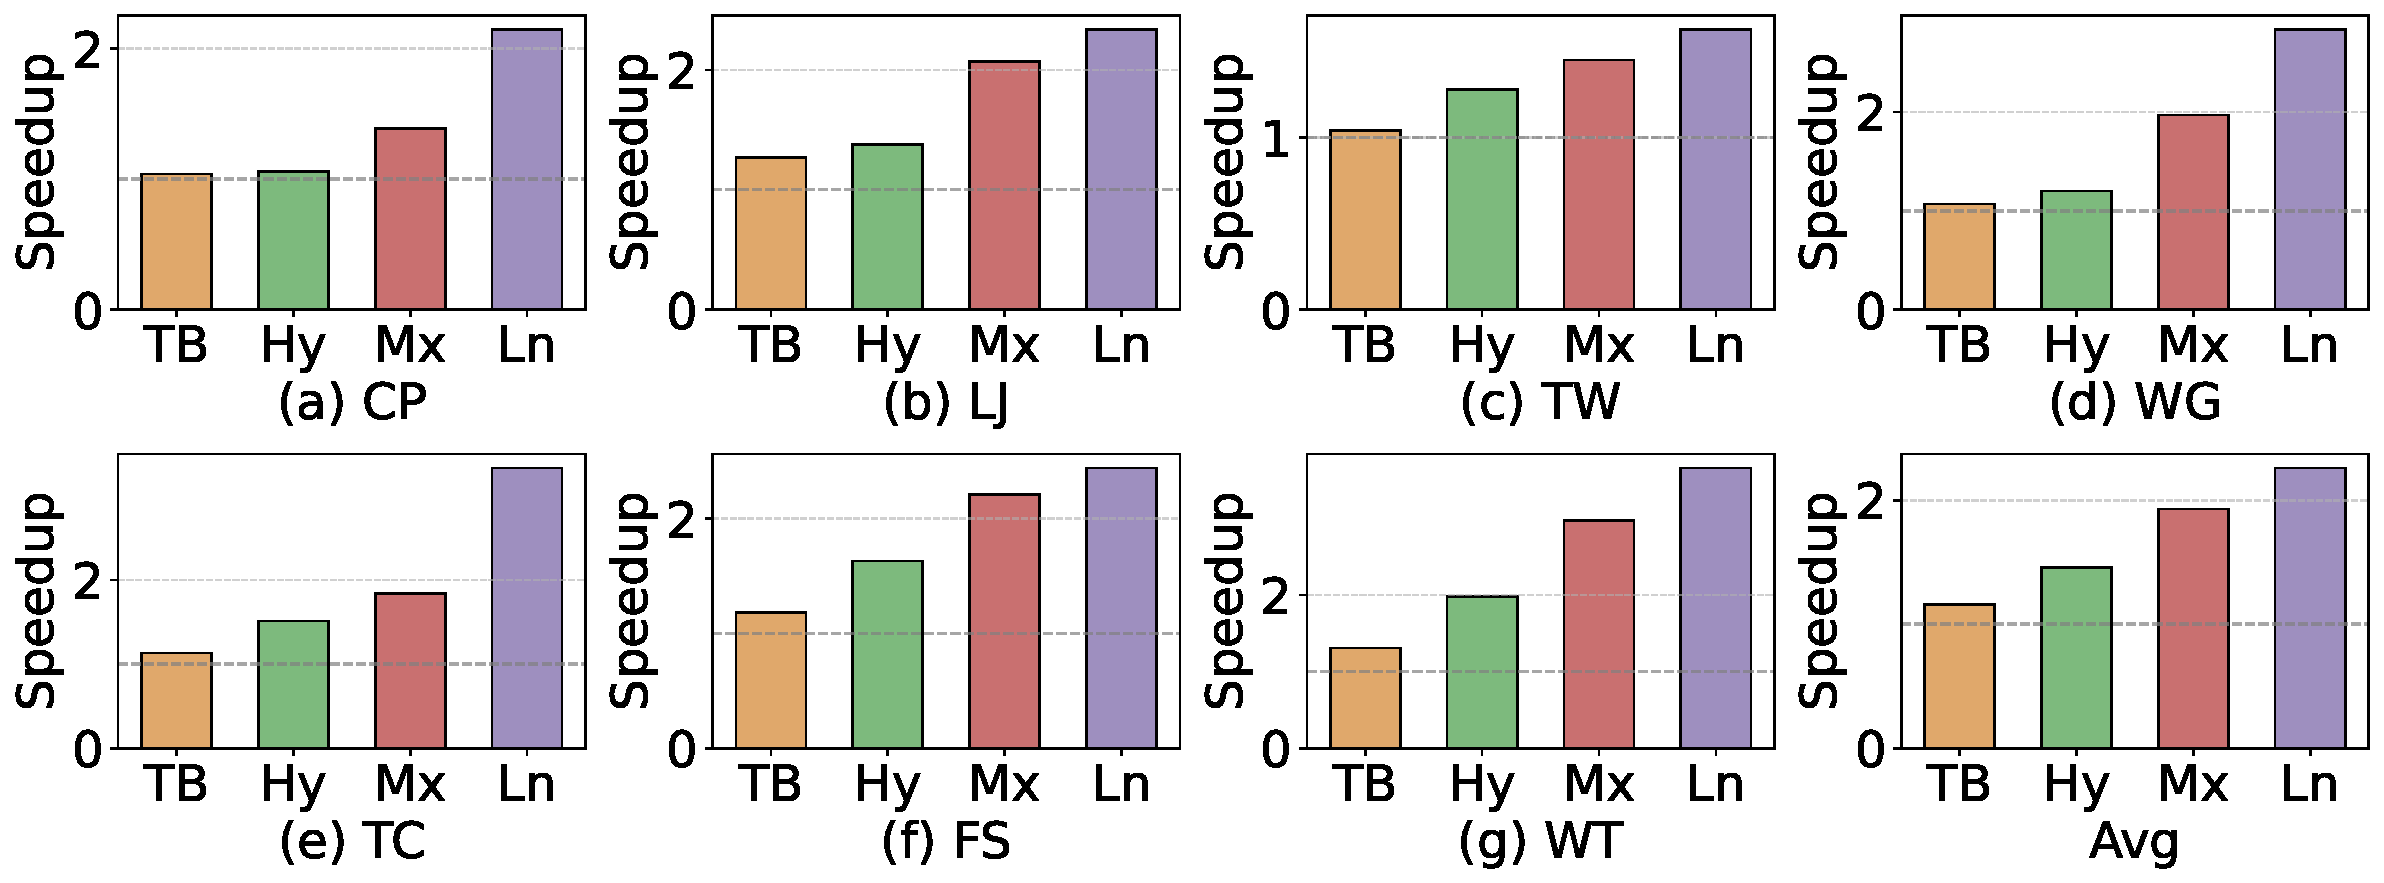
\includegraphics[width=1\linewidth]{figures/bfs_speedup_cropped.pdf}
%     \caption{Incremental speedups under progressive GIR optimizations for BFS, including TB, +Hy, +Mx, +Ln, respectively.}
%     % Each bar shows the cumulative speedup contributed by each technique (TB, +Hy, +Mx, +Ln) over a plain parallel BFS baseline.}
%     \label{fig:bfs_ablation}
% \end{figure}


% Figure~\ref{fig:bfs_ablation} reports the cumulative speedup at each stage for all seven graphs plus the average.
% Each technique contributes meaningfully, and the gains compound across the four stages.

% \textbf{TB} provides a moderate but consistent first-stage improvement.
% Graphs with large, dense frontiers (LJ, FS, WT) benefit the most, as switching from top-down to bottom-up traversal avoids redundant edge checks during peak frontier expansion.
% LJ reaches $1.27\times$ and WT reaches $1.31\times$ speedup over the plain BFS baseline at this stage.
% On TW, where the dominant SCC is extremely large, TB alone already reaches $1.04\times$, confirming that even a large frontier benefits modestly from direction switching.

% \textbf{+Hy} yields larger gains on graphs with a structurally dominant large block.
% Because the GIR hierarchy makes the largest BiCC block explicit, the hybrid strategy is applied selectively to that one block without disturbing the rest.
% WT jumps from $1.31\times$ to $1.98\times$ at this stage, and FS from $1.18\times$ to $1.63\times$, reflecting the high structural skewness of these social graphs where a single giant block dominates traversal cost.
% On CP and TC, which have a more uniform block-size distribution, the Hy gain is smaller ($1.0\times$ increment), since no single block is dominant enough to warrant a dedicated hybrid strategy.

% \textbf{+Mx} delivers the largest single-stage speedup increase across nearly all datasets.
% By dedicating threads to the largest block, this stage fully exposes the task parallelism that GIR's block decomposition provides.
% LJ reaches $2.07\times$ cumulative speedup, WG reaches $1.97\times$, and WT reaches $2.97\times$, all jumping by at least $0.7\times$ over the previous stage.
% TW's modest gain to $1.45\times$ reflects the limited number of independent blocks in its graph structure.

% \textbf{+Ln} provides the final speedup increment by replacing the parallel BFS kernel with a sequential linear scan for small blocks, eliminating synchronization overhead that dominates at small scales.
% TC benefits the most here, jumping from $1.84\times$ to $3.33\times$—the largest single-stage jump in the experiment—consistent with TC's exceptionally high count of small, loosely connected BiCC blocks.
% WT reaches its final $3.7\times$ speedup, the highest across all datasets, driven by both Hy and Ln acting on its highly skewed block-size distribution.

% Overall, the fully optimized configuration achieves speedups of $1.6\times$ (TW) to $3.7\times$ (WT), with an average of $2.3\times$ across all seven graphs (the Avg panel).
% The staircase pattern visible in every panel of Figure~\ref{fig:bfs_ablation} confirms that none of the four techniques is redundant: each addresses a distinct source of inefficiency exposed by the GIR hierarchy, and together they deliver substantial end-to-end acceleration.

\subsection{Scalability}
\begin{figure}[t]
    \centering
    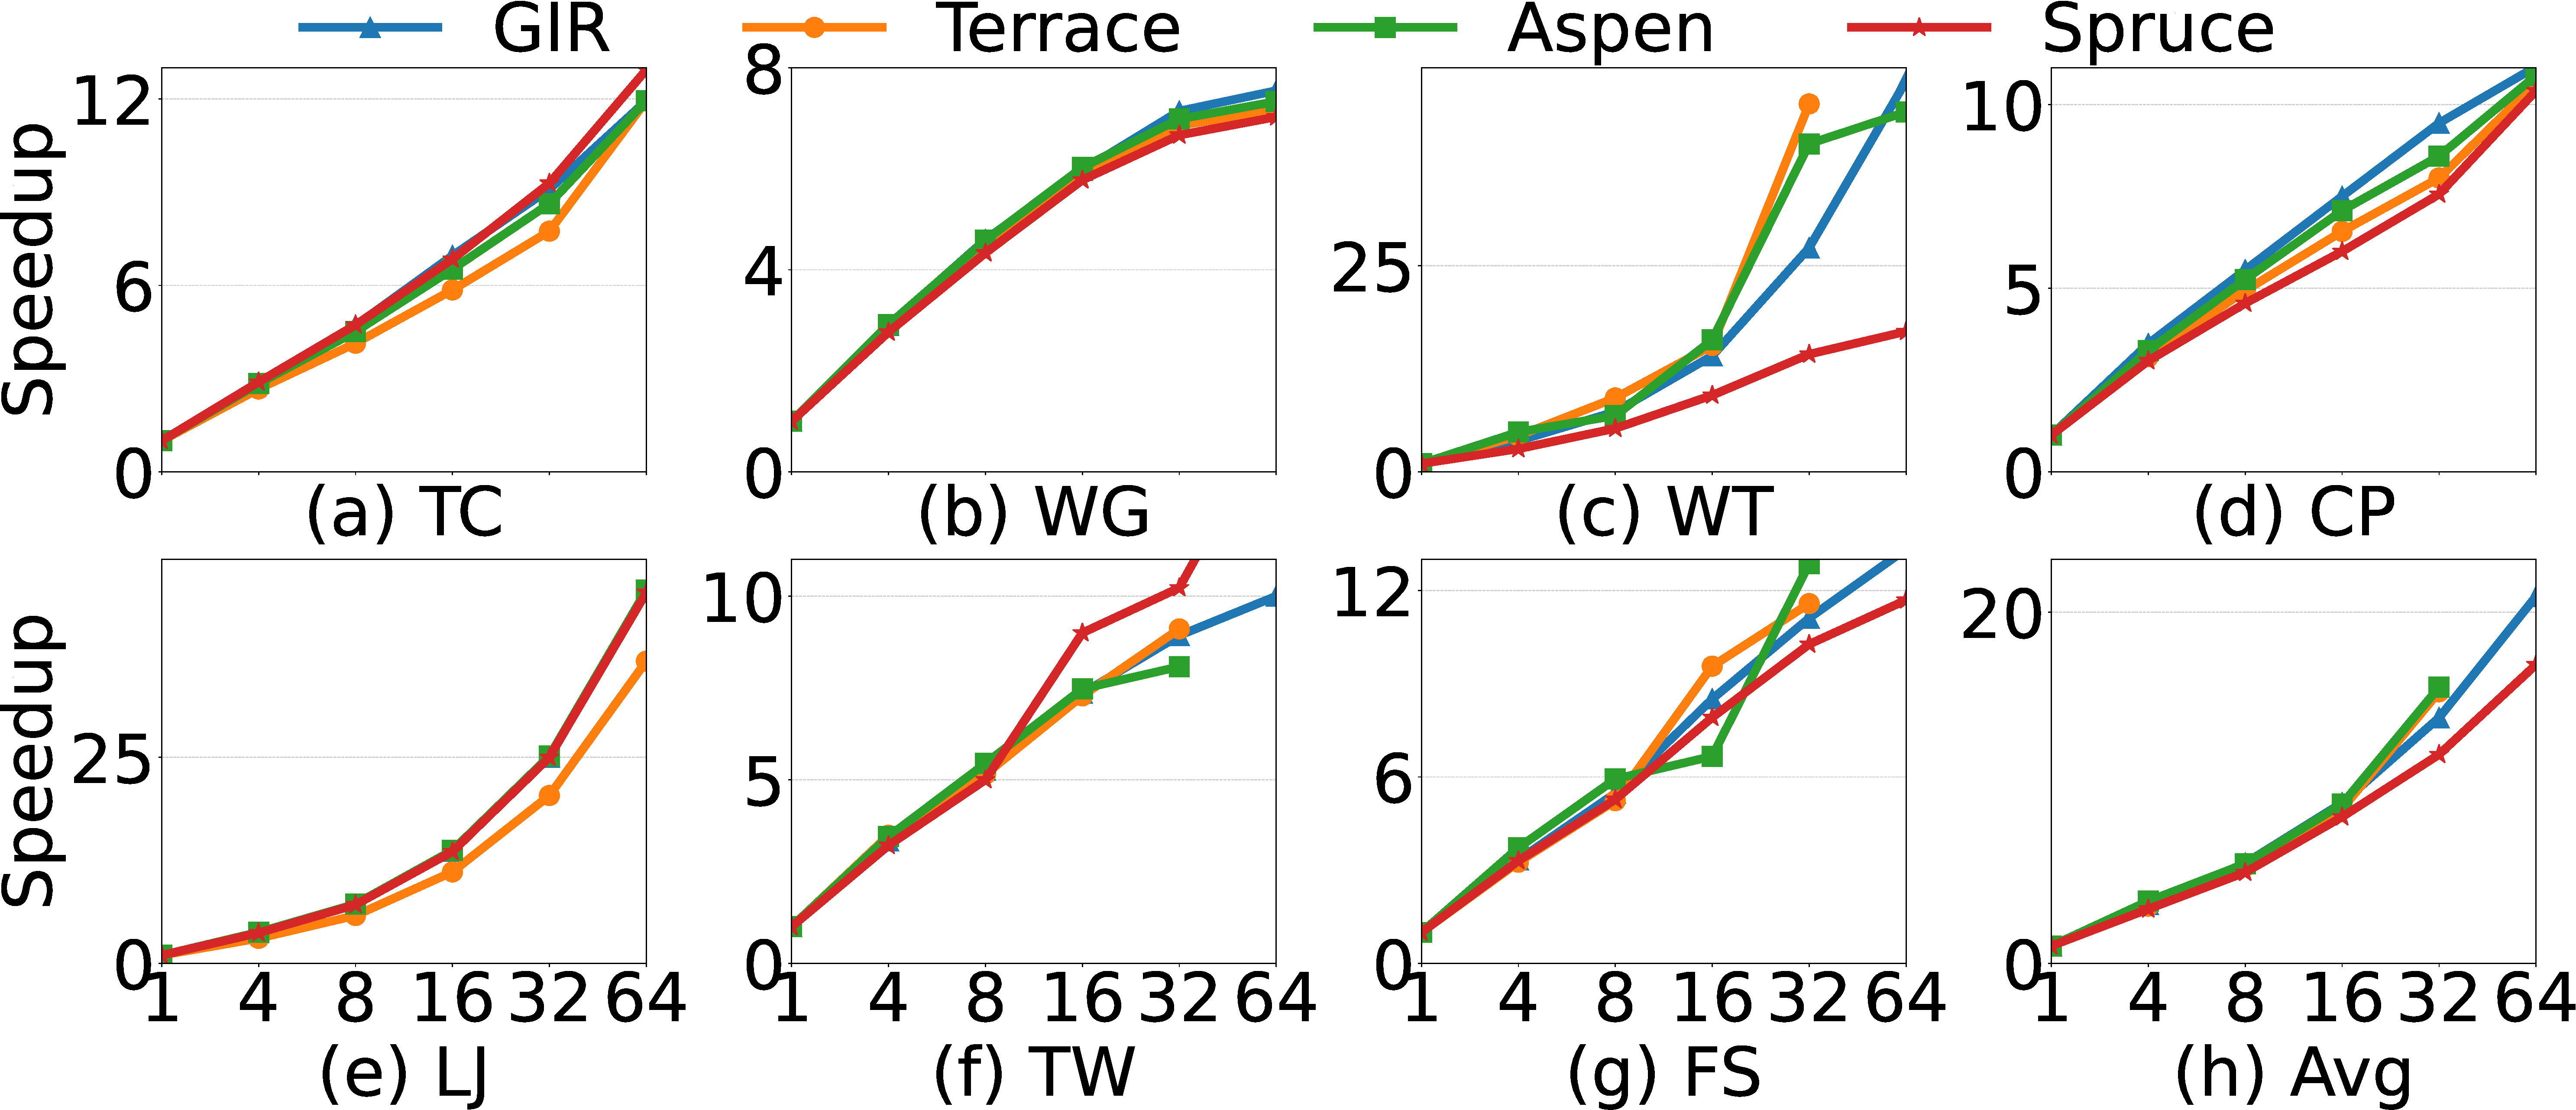
\includegraphics[width=1\linewidth]{figures/multiple_thread_speedup_all-crop.pdf}
    \caption{The BFS scalability against thread number. For TW and FS, Terrace and Aspen fail at 64 threads. For WT, Terrace fails at 64 threads.}
    \Description{Line charts of BFS speedup versus thread count (1 to 64) for GIR, Terrace, Aspen, and Spruce across seven datasets and their average.}
    % \caption{Multi-threaded BFS speedup of GIR, Terrace, Aspen, and Spruce on all seven datasets as the thread count increases from 1 to 64, where each system is normalized to its own single-threaded runtime.
    % For TW and FS, Terrace and Aspen fail at 64 threads; for WT, only Terrace fails at 64 threads.
    % Panel (h) shows the average speedup across all datasets; Terrace and Aspen averages are plotted only up to 32 threads.}
    \label{fig:mt_speedup}
\end{figure}


%We test the downstream graph query scalability by varying the number of threads from 1 to 64 across all seven datasets.
%Figure~\ref{fig:mt_speedup} shows the BFS speedup.
% normalized to GIR's single-threaded runtime.
%Note that all systems fail at 64 threads on TW and FS (the two largest graphs), and Terrace fails at 64 threads on WT. \YJ{Mismatch with the numbers reported in Table IV.}
% those curves are truncated at 32 threads accordingly.
%We make three observations.

We test the scalability of GIR by varying the number of threads from 1 to 64 across all seven datasets.
We take the BFS as a representative example.
Figure~\ref{fig:mt_speedup} shows the speedup of each method normalized to its own single-thread runtime.
Note that Terrace and Aspen fail at 64 threads on TW and FS, and Terrace fails at 64 threads on WT.
% their curves are truncated accordingly. 
% \YJ{Mismatch with the numbers reported in Table IV.}


% (i) GIR achieves the steepest scaling on graphs with many independent BiCC blocks.
% On WT (Figure~\ref{fig:mt_speedup}(c)), GIR reaches $47.4\times$ at 64 threads, ahead of Aspen ($43.6\times$) and Spruce ($17.0\times$).
% On LJ (Figure~\ref{fig:mt_speedup}(e)), all systems scale similarly well, with GIR reaching $45\times$ at 64 threads.
% On TC (Figure~\ref{fig:mt_speedup}(a)), GIR reaches $11.9\times$ at 64 threads, consistent with TC's exceptionally high count of small BiCC blocks.
% This steep scaling is driven by GIR's block-level task decomposition: each additional thread picks up independent block tasks with minimal inter-task coordination.

Particularly, we make three observations.
\textit{(i)} On average, GIR achieves $20.9\times$ speedups with 64 threads, way higher than Spruce's $17\times$.
Terrace and Aspen achieve $15.5\times$ and $15.7\times$ with 32 threads, respectively. They are omitted at 64 threads due to failures on TW and FS.


% The average scaling confirms GIR's strong aggregate scaling. 
% GIR's average speedup reaches $20.9\times$ from 1 to 64 threads, while Spruce reaches $17.0\times$. 
% Terrace and Aspen average reaches $15.5\times$ and $15.7\times$ from 1 to 32 threads, respectively.  
% they are omitted at 64 threads due to failures on TW and FS.

% The average scaling confirms GIR's strong aggregate scaling. 
% GIR's average speedup reaches $20.9\times$ from 1 to 64 threads, while Spruce reaches $17.0\times$. 
% Terrace and Aspen average reaches $15.5\times$ and $15.7\times$ from 1 to 32 threads, respectively.  
% they are omitted at 64 threads due to failures on TW and FS.

\textit{(ii)} GIR achieves the highest scaling on graphs with many independent BiCC blocks.
On WT, GIR achieves $47.4\times$ at 64 threads, higher than Aspen ($43.6\times$) and Spruce ($17\times$).
On LJ, all methods scale similarly well, with GIR reaching $45\times$ at 64 threads.
On TC, GIR achieves $11.9\times$ at 64 threads, mainly due to TC's exceptionally high count of small BiCC blocks.
% This steep scaling is driven by GIR's block-level task decomposition: each additional thread picks up independent block tasks with minimal inter-task coordination.

% (ii) GIR achieves the highest scalability on graphs with many independent BiCC blocks.
% On LJ and WT, GIR achieves $45\times$ and $47.4\times$ speedups at 64 threads, respectively, much higher than other baselines.
% On TC, which has an exceptionally high count of small BiCC blocks, GIR reaches $11.9\times$ at 64 threads with the largest gap over Spruce ($3\times$ from Table~\ref{tab:speedup_summary_alg}).
% This steep scaling is driven by GIR's block-level task decomposition: each additional thread picks up independent block tasks with minimal inter-task coordination.

\textit{(iii)} Scaling is more modest on graphs dominated by a few large SCCs.
On WG and CP, all methods scale similarly, with GIR reaching $7.5\times$ and $11\times$ at 64 threads.
On TW and FS, GIR achieves $8.9\times$ and $11.1\times$ at 32 threads before Terrace and Aspen fail to scale further.
% The limited block count in these graphs bounds the available task parallelism. 

% (i) GIR achieves the highest scalability on graphs with many independent BiCC blocks.
% On LJ and WT, GIR achieves $45\times$ and $47.4\times$ speedups at 64 threads, respectively, much higher than other baselines.
% On TC, which has an exceptionally high count of small BiCC blocks, GIR reaches $11.9\times$ at 64 threads with the largest gap over Spruce ($3\times$ from Table~\ref{tab:speedup_summary_alg}).
% This steep scaling is driven by GIR's block-level task decomposition: each additional thread picks up independent block tasks with minimal inter-task coordination.

%(i) GIR achieves the highest scalability on graphs with many independent BiCC blocks.
%On LJ and WT, GIR achieves $45\times$ and $47.4\times$ speedups at 64 threads, respectively, much higher than other baselines.
%On TC, which has an exceptionally high count of small BiCC blocks, GIR reaches $11.9\times$ at 64 threads with the largest gap over Spruce ($3\times$ from Table~\ref{tab:speedup_summary_alg}).
%This steep scaling is driven by GIR's block-level task decomposition: each additional thread picks up independent block tasks with minimal inter-task coordination.

%(ii) Scaling is more modest on graphs dominated by a few large SCCs.
%On WG and CP (Figure~\ref{fig:mt_speedup}(b)(d)), GIR reaches $7.3\times$ and $10.7\times$ at 64 threads.
%On TW and FS (Figure~\ref{fig:mt_speedup}(f)(g)), GIR reaches $8.9\times$ and $11.1\times$ at 32 threads before all systems fail to scale further.
%The limited block count in these graphs bounds the available task parallelism, but GIR still consistently leads all baselines at every thread count.

%(iii) The average panel (Figure~\ref{fig:mt_speedup}(h)) confirms that GIR's advantage compounds with thread count.
%GIR's average speedup reaches $24.5\times$ at 64 threads, while Spruce reaches $13.5\times$.
%Terrace and Aspen averages are omitted at 64 threads due to failures on multiple datasets.



% \subsection{Others?}
% \YJ{I would suggest we report as many expeirimental results as possible.}

%
%1. the distribution time of different size of blocks, 
%the total number of blocks are 1545753	
%biggest one is 824847	
%second one is 375651	
%third one is 686	
%fourth one 531	
%fifth one 348	
%...301	
%...98	
%the total number of BiCC with size 2 is 1100134	

\section{Related Work}
\label{sec: related work}
% \subsection{Dynamic Graph Systems}
% \label{subsec:dynamic}
% ============================================================
% \YJ{Discuss other related works: CuckooGraph, etc.}

\begin{maybecut}
\textit{Dynamic graph computation.}
Besides the extensively discussed Terrace~\cite{pandey2021terrace},
Spruce~\cite{shi2024spruce}, Aspen~\cite{dhulipala2019low},
GraphBolt~\cite{mariappan2019graphbolt}, and DZiG~\cite{mariappan2021dzig},
Stinger~\cite{ediger2012stinger} aggregates edge lists into
fixed-size blocks with a hash-table index for point queries.
GraphOne~\cite{kumar2020graphone} combines an adjacency list with
an edge log that is periodically merged in batches.
Sortledton~\cite{fuchs2023sortledton} replaces edge lists with an
unrolled skip list offering $O(\log|E|)$ update and lookup with
transactional support.
Teseo~\cite{de2021teseo} uses packed memory arrays as leaves of
B+ trees with optimistic locking for concurrent access.
CuckooGraph~\cite{fan2025cuckoograph} proposes a hash-array-based
structure that adaptively resizes through transformation and denylist
techniques.
Other works include LiveGraph~\cite{zhu2019livegraph} and
LLAMA~\cite{macko2015llama}.
% CUT CANDIDATE: none of these are experimental baselines (only
% Terrace/Spruce/Aspen/GraphBolt/DZiG are); condensed in \texttt{fixed} below.
\end{maybecut}
\begin{fixed}
\textit{Dynamic graph computation.}
Besides the extensively discussed Terrace~\cite{pandey2021terrace},
Spruce~\cite{shi2024spruce}, Aspen~\cite{dhulipala2019low},
GraphBolt~\cite{mariappan2019graphbolt}, and DZiG~\cite{mariappan2021dzig},
several other systems propose specialized storage structures for dynamic
graphs, including Stinger~\cite{ediger2012stinger} (hash-indexed edge
blocks), GraphOne~\cite{kumar2020graphone} (adjacency list with a batched
edge log), Sortledton~\cite{fuchs2023sortledton} (unrolled skip list),
Teseo~\cite{de2021teseo} (packed memory arrays with optimistic locking),
CuckooGraph~\cite{fan2025cuckoograph} (adaptive hash-array resizing),
LiveGraph~\cite{zhu2019livegraph}, and LLAMA~\cite{macko2015llama}.
\end{fixed}



\textit{Query-dependent incremental computation.}
A separate line of work attempts to reuse prior computational results
across updates~\cite{besta2021practice,ramalingam1996computational}.
\textit{Khanda et al.}~\cite{khanda2021parallel} maintain an SSSP
tree rooted at a fixed source after each update, recomputing only the
affected subtree.
\textit{Kickstarter}~\cite{vora2017kickstarter} retains approximate monotonic
results and propagates corrections for invalidated values.
% \cq{ 
\textit{GraphBolt}~\cite{mariappan2019graphbolt} uses dependency-driven
synchronous processing: it tracks per-vertex aggregation dependencies across
BSP iterations and propagates only the delta caused by mutations, supporting
algorithms including PageRank, belief propagation, SSSP, and BFS.

\textit{DZiG}~\cite{mariappan2021dzig} extends GraphBolt with sparsity-aware
processing that skips zero-contribution edges during incremental propagation,
reducing redundant work on sparse updates.
\begin{maybecut}
\textit{RisGraph}~\cite{feng2021risgraph} targets sub-millisecond per-update
analysis by streaming graph mutations into a compact active-vertex frontier.
\textit{GraphFly}~\cite{chen2022graphfly} uses asynchronous dependency-flow
execution to reduce synchronization overhead in streaming graph processing.
\textit{IncBoost}~\cite{yin2024incboost} focuses on incremental processing
under edge deletions and weight updates.
\textit{Fan et al.}~\cite{fan2021incrementalizing} propose a general framework
for incrementalizing arbitrary graph algorithms by detecting affected
regions across updates.
\textit{Bauer and Wagner}~\cite{bauer2009batch} study batch dynamic SSSP
experimentally, showing reuse is only effective when the affected
subgraph is small.

For betweenness centrality specifically, \textit{Green et al.}~\cite{green2012fast}
track path-count changes caused by each edge insertion or deletion to maintain
an incremental BC score, while \textit{Nasre et al.}~\cite{Nasre2014IncBC}
give an asymptotically faster incremental BC algorithm that exploits DAG structure
to localize the repair.
% CUT CANDIDATE: none of these are experimental baselines (unlike Khanda
% et al./Kickstarter/GraphBolt/DZiG above); condensed in \texttt{fixed} below.
\end{maybecut}
\begin{fixed}
Other systems in this space target complementary goals: sub-millisecond
per-update latency~\cite{feng2021risgraph}, asynchronous dependency-flow
execution~\cite{chen2022graphfly}, incremental processing under deletions
and weight updates~\cite{yin2024incboost}, general frameworks for
incrementalizing arbitrary algorithms~\cite{fan2021incrementalizing},
batch dynamic SSSP~\cite{bauer2009batch}, and incremental betweenness
centrality~\cite{green2012fast,Nasre2014IncBC}.
\end{fixed}
All of these systems maintain algorithm-specific state (e.g., per-vertex
aggregation values, SSSP trees, path-count tables, or monotonic approximations)
that must be reset or rebuilt when the algorithm or source changes.
GIR instead maintains \emph{algorithm-agnostic} structural invariants
(WCC, SCC, BiCC) that benefit BFS, SSSP, and BC simultaneously, with no
per-algorithm reconfiguration.
% }

\begin{maybecut}
\textit{Theoretical dynamic graph algorithms.}
A substantial body of theory addresses fully dynamic connectivity; we refer
to Hanauer et al.~\cite{Hanauer2022DynSurvey} for a comprehensive survey.
\textit{Holm et al.}~\cite{holm2001poly} give poly-logarithmic deterministic
algorithms for dynamic connectivity, MST, 2-edge connectivity, and
biconnectivity.
\textit{Wulff-Nilsen}~\cite{wulff2013faster} improves the deterministic
connectivity bound.
\textit{De Man et al.}~\cite{de2025towards} study batch-dynamic
connectivity in a practical parallel setting, targeting throughput on
large batches of concurrent edge updates.
These algorithms target worst-case update complexity under arbitrary adversarial
sequences.
% CUT CANDIDATE: theoretical worst-case algorithms, not empirical baselines;
% condensed in \texttt{fixed} below.
\end{maybecut}
\begin{fixed}
\textit{Theoretical dynamic graph algorithms.}
A substantial body of theory addresses fully dynamic connectivity, MST, and
biconnectivity with poly-logarithmic worst-case guarantees under arbitrary
adversarial update
sequences~\cite{Hanauer2022DynSurvey,holm2001poly,wulff2013faster,de2025towards}.
\end{fixed}
GIR's maintenance is not designed to match these worst-case guarantees; instead,
it exploits the SPU five-case classification to achieve \emph{low average-case
cost} on real-world graphs, where most updates fall into cheap cases (Case 1
or Case 4) and full structural repair is rare.
Unlike purely theoretical constructions, GIR integrates maintenance with a
two-level parallel execution framework and is evaluated end-to-end on real
graph workloads.
% These approaches can be highly efficient when the same algorithm is
% repeated from the same source, but they are tightly coupled to a
% specific algorithm and, in some cases, a specific source node.
% In practice, dynamic graph workloads involve ad hoc queries with
% varying sources, targets, and algorithms~\cite{Hanauer2022DynSurvey},
% so such query-dependent systems offer limited reuse.


% \textbf{Intermediate representations and graph frameworks.}
\textit{Intermediate representations (IRs)}, such as LLVM
IR~\cite{Lattner2004LLVM}, decouple source languages from back-end
optimization passes, enabling reusable analysis across many
compilation stages.
% GIR is directly inspired by this principle: just as a compiler IR is
% computed once and reused across many passes, GIR maintains structural
% invariants once and makes them available to many downstream
% algorithms.
Several graph domain-specific languages adopt a related
algorithm-execution separation.
GraphIt~\cite{Zhang2018GraphIt} separates algorithm descriptions from
scheduling decisions.
Galois~\cite{nguyen2013lightweight} decouples
operator logic from parallel execution policies.
Ligra~\cite{Shun2013Ligra}, Green-Marl~\cite{hong2012green},
Gemini~\cite{zhu2016gemini}, and Pregel~\cite{malewicz2010pregel}
target shared- and distributed-memory execution on static snapshots.

% Unlike these frameworks, GIR is not a programming abstraction or a
% scheduling layer.
% Instead, it is a persistent structural layer maintained
% incrementally under continuous updates and exposed directly to
% downstream algorithms.
% No existing system simultaneously maintains multi-granular,
% query-agnostic structural invariants, repairs them incrementally
% under dynamic updates, and exposes them for task-parallel query
% execution. This is the gap GIR fills.


% Terrace~\cite{pandey2021terrace},
% Aspen~\cite{dhulipala2019low}, and Spruce~\cite{shi2024spruce}
% (evaluated as baselines in Section~\ref{sec:experiment}) take
% complementary storage-layer approaches.
% All of these systems optimize for update throughput at the storage
% layer but provide no persistent structural invariants for downstream
% analytics.

% CuckooGraph~\cite{fan2025cuckoograph} proposes a hash-array-based structure for large-scale dynamic graphs that adaptively resizes through TRANSFORMATION and DENYLIST techniques, achieving high insertion throughput with low memory overhead.
% Like Terrace, Spruce, and Aspen, CuckooGraph is optimized purely for storage-level update performance and does not maintain any structural invariants for downstream analytics.
% Several other adjacency-list-based systems have been proposed for dynamic graph storage.
% Stinger~\cite{ediger2012stinger} aggregates edge lists into fixed-size blocks and uses a
% hash table as a secondary index to improve point query efficiency.
% GraphOne~\cite{kumar2020graphone} combines an adjacency list with an edge log array:
% updates are appended to the log and periodically merged into the adjacency list in batches,
% supporting real-time analytics on evolving graphs.
% LiveGraph~\cite{zhu2019livegraph} stores edges in purely sequential transactional edge logs,
% optimizing sequential scan performance for read-heavy workloads.
% Sortledton~\cite{fuchs2023sortledton} replaces edge lists with an unrolled skip list,
% providing $O(\log|E|)$ lookup, insertion, and deletion with transactional support.
% Teseo~\cite{de2021teseo} uses packed memory arrays as leaves of B$^+$ trees and
% supports concurrent reads and writes through optimistic locking.
% LLAMA~\cite{macko2015llama} takes a snapshot-oriented approach,
% storing graph versions as large multiversioned arrays to support
% efficient analytics on historical snapshots.
% Like CuckooGraph, Terrace, Spruce, and Aspen, all of these systems target update throughput
% at the storage layer and provide no persistent structural invariants for downstream analytics.

% Dynamic graph systems must support two operations: integrating
% structural updates quickly and answering downstream queries
% efficiently.
% Existing systems focus primarily on the first operation.
% We survey the most relevant systems and explain their limitations
% for the second operation.

% \textbf{Graph storage systems.} 
% % \YJ{They should not be called "storage system".}
% Most dynamic graph systems propose specialized in-memory data
% structures that balance update cost, query efficiency,
% and memory usage.
% Static representations such as CSR and CSC~\cite{wheatman2018packed}
% store adjacency information in contiguous arrays and enable
% efficient traversal, but edge insertions and deletions require
% rebuilding large arrays, which is prohibitively expensive
% under frequent updates.

% Terrace~\cite{pandey2021terrace} targets skewed streaming graphs.
% It introduces a hierarchical adjacency representation in which
% a vertex's neighbors are stored using different data structures
% depending on its degree.
% As degrees evolve, the system dynamically reorganizes storage
% to improve locality and update efficiency on power-law graphs.
% However, Terrace focuses entirely on storage and does not
% maintain any structural invariants for downstream computation.

% Spruce~\cite{shi2024spruce} combines compact indexing with
% update-friendly adjacency organization.
% It integrates dynamic buffers with CSR-like sorted blocks and
% introduces a read-optimized concurrency protocol that supports
% efficient simultaneous reads and writes.
% Like Terrace, Spruce targets update throughput and leaves
% downstream analytics to be rerun from scratch after each update.

% Aspen~\cite{dhulipala2019low} represents graphs using compressed purely
% functional trees and exposes immutable snapshot views for
% analytics.
% Each update produces a new graph version, enabling concurrent
% readers on consistent snapshots while preserving structural
% sharing across versions.
% This versioning design is well suited for analytics on static
% snapshots, but it does not maintain structural invariants
% incrementally and requires full recomputation for downstream
% algorithms after each update.

% \YJ{Avoid duplicates. If they have been discussed in detail earlier, we can simply mention them here.}

% \textbf{Query-dependent computation systems.}
% Another line of work attempts to reuse prior computational
% results directly~\cite{besta2021practice,ramalingam1996computational}.
% For example, \textit{Khanda et al.}~\cite{khanda2021parallel} maintains an SSSP tree
% rooted at a fixed source after each query. %people--> according to the first
% After a graph update, it identifies the affected subtree and
% recomputes only that portion.
% Kickstarter~\cite{vora2017kickstarter} retains approximate monotonic
% computation results across updates, trimming values that have been
% invalidated by edge deletions and propagating corrections only
% within the affected region.
% Green et al.~\cite{green2012fast} maintain an incremental
% betweenness centrality score by tracking only the path-count
% changes caused by each edge insertion or deletion.
% Fan et al.~\cite{fan2021incrementalizing} propose a general framework
% for incrementalizing arbitrary graph algorithms by detecting affected
% regions and reusing unaffected partial results across updates.
% Bauer and Wagner~\cite{bauer2009batch} study batch dynamic SSSP algorithms
% experimentally, showing that incremental updates outperform recomputation
% only when the affected subgraph remains small relative to the full graph.
% These approaches are efficient when the same query is repeated
% under the same algorithm.
% However, each is tightly coupled to a specific algorithm and,
% in some cases, a specific source node.
% If the query algorithm or source changes, the cached state
% provides no benefit.
% In practice, dynamic graph workloads involve ad hoc queries
% with varying sources, targets, and algorithms~\cite{Hanauer2022DynSurvey},
% so such query-dependent systems offer limited reuse.

% % \YJ{Double check which 2-extreme does each method belong to.}

% % \textbf{GIR's position.}
% % GIR differs from all of these systems in one key respect.
% % Storage systems such as Terrace, Spruce, and Aspen are
% % history-blind: they discard all prior structural computation
% % after each update.
% % Query-dependent systems preserve results but tie them to
% % a specific query and source.
% % GIR occupies the middle ground: it maintains a small set of
% % query-agnostic structural invariants that persist across updates
% % and benefit many downstream algorithms without being tied to
% % any specific query or source.
% % GIR is designed to operate on top of existing storage systems
% % rather than replace them.
% % It can be integrated with formats such as Terrace, Aspen,
% % Spruce, and others~\cite{bender2007adaptive,king2016dynamic,islam2023dgap} as a
% % structural layer above the storage layer.

% % % ============================================================
% % \subsection{Intermediate Representations for Graphs}
% % ============================================================

% % \textbf{Intermediate representation in compilers.}
% % Compiler intermediate representations (IRs), such as LLVM IR~\cite{Lattner2004LLVM}, decouple source languages from optimization passes.
% % This abstraction enables reusable analysis and transformation across different compilation stages.\YJ{Discuss any works that either call or relate to IR for Graph} Several graph DSLs and compilers, such as GraphIt~\cite{Zhang2018GraphIt}, provide scheduling abstractions that separate algorithm specification from execution optimization. \YJ{Only one? Any others?}
% % However, these systems primarily focus on optimizing computation rather than maintaining persistent structural invariants under dynamic updates.

% % ============================================================

% % \textbf{Inter}
% \textbf{Intermediate representations (IRs)}, 
% % in compilers.}
% % Compiler intermediate representations (IRs), 
% such as LLVM
% IR~\cite{Lattner2004LLVM}, decouple source languages from
% back-end optimization passes.
% This abstraction enables reusable analysis and transformation
% across compilation stages.
% A key property of compiler IRs is that they are computed once
% and reused across many passes, rather than recomputed from
% source on every pass.
% % \textbf{Graph DSLs and scheduling abstractions.}
% Several graph domain-specific languages adopt a similar
% separation between algorithm specification and execution
% strategy.
% GraphIt~\cite{Zhang2018GraphIt} separates graph algorithm
% descriptions from scheduling decisions such as direction
% optimization, NUMA-awareness, and cache tiling.
% Galois~\cite{nguyen2013lightweight} provides a worklist-based runtime
% that separates operator logic from parallel execution policies.
% Ligra~\cite{Shun2013Ligra} provides a unified interface for
% vertex-subset-based graph algorithms on shared memory.
% Green-Marl~\cite{hong2012green} provides a domain-specific language
% with a property graph model that compiles to efficient parallel C++ code.
% Gemini~\cite{zhu2016gemini} targets distributed-memory execution with
% chunk-based graph partitioning.
% Pregel~\cite{malewicz2010pregel} introduces a vertex-centric bulk synchronous parallel model for large-scale graph processing.
% These systems improve programmability and performance for
% static graph analytics.
% However, they operate on fixed graph snapshots~\cite{mccune2015thinking}.
% They do not maintain persistent structural invariants across
% updates, and they require each downstream algorithm to
% rebuild structural knowledge from scratch.

% \textbf{GIR's distinction.}
% GIR adopts the IR philosophy and applies it to dynamic graphs.
% Like a compiler IR, GIR is computed incrementally and reused
% across many downstream operations.
% Unlike graph DSLs, GIR is not a programming abstraction.
% It is a persistent structural layer that is maintained under
% continuous updates and that exposes structural invariants
% directly to downstream algorithms.
% No prior dynamic graph system maintains a multi-granular,
% query-agnostic structural layer of this kind.
% This is the gap that GIR fills.
\section{Dicussion and Limitation}
\label{sec:discussion}

% \subsection{Dicussion}

% \YJ{TODO. This is more like dicussion. Should them be here, merge with the next section, or move to else where.}

% The three levels are mutually complementary.
% WCC prunes at the global level, 
% SCC prunes directed reachability and eliminates
% cycles, and BC tree decomposes the remaining work into parallel tasks
% and localizes maintenance.

\textit{Algorithm independence.}
The three structural layers in GIR do not depend on any specific query
source, target, or algorithm.
The DAG and BC trees are maintained unconditionally
after each graph update.
Any downstream algorithm can use these structures without
prior knowledge.
% of what other algorithms have run.

\textit{Integration with other dynamic graph systems.}
GIR is designed to operate above existing dynamic graph representation
systems, not to replace them.
It can be integrated with formats such as
PMA~\cite{bender2007adaptive},
DCSR~\cite{king2016dynamic},
Terrace~\cite{pandey2021terrace}, and
DGAP~\cite{islam2023dgap}.
The storage layer is responsible for maintaining adjacency data
efficiently under updates.
GIR is responsible for maintaining the structural invariants.
This separation improves modularity and allows GIR to be added to an existing system without redesigning the storage stack.

\textit{Experimental update model.}
\wastext{Our experiments follow the standard evaluation protocol in the dynamic graph systems literature: updates are randomly generated edge insertions and deletions~\mbox{\cite{pandey2021terrace,shi2024spruce,dhulipala2019low}}.
This protocol is widely adopted because large-scale real-world streaming traces are often proprietary or unavailable for the graph sizes we target.
Randomly generated updates exercise the system uniformly and provide reproducible benchmarks, but they may not capture locality or burstiness patterns present in real streams.
Evaluating GIR on temporal graph benchmarks (e.g., Wikipedia edit histories or Reddit interaction streams) is a natural extension for future work.}
\fixtext{Rather than generating synthetic insertions and deletions independent of the
graph's own structure, for each graph we hold out 50\% of its edges, build
GIR on the remaining 50\% to obtain an initial fixed point, and then stream
the held-out half back in as insertions; deletions are sampled from the
loaded half. Because both the streamed insertions and the sampled
deletions are real edges drawn from the graph itself, this exercises GIR
under the same structural distribution (degree skew, locality) it will see
in the final graph, unlike edge pairs drawn independently at random. We
shuffle the streamed order to avoid artifacts from the original edge-list
ordering and eliminate locality effects in the stream. Real production
traces (e.g., timestamped edit histories) remain out of scope here, as
they are largely proprietary or unavailable at the graph sizes we target;
this protocol is the closest practical substitute.}

\textit{Extensibility.}
The current instantiation of GIR uses WCC, SCC, and BiCC because
they provide a strong balance between expressiveness and
computational feasibility at scale.
The framework is not limited to these three.
Additional structural indices, such as dominator trees or
reachability indices, can be incorporated when they provide
value for a target workload.


\cq{\textit{Workload scope.}
The current evaluation covers traversal-based algorithms (BFS, SSSP, BC), which align naturally with GIR's structural decomposition.
Mining and pattern-matching tasks, such as dense subgraph discovery or subgraph isomorphism, have different computational characteristics and do not immediately exploit the condensation DAG or BC tree in the same way.
We expect that WCC partitioning could still reduce search space for such tasks, but the precise benefit depends on the algorithm.
Extending GIR to support mining workloads is left for future work.}

% \subsection{Scope of Benefit}
% The three GIR levels provide three types of structural knowledge that enable three corresponding optimizations.

% \textit{WCC (Level 1) is for scope elimination}. Any single-source algorithm on a directed or undirected graph can immediately discard all WCCs that do not contain the source. This benefits many algorithms, such as, BFS, DFS, SSSP, APSP (per-source), reachability queries, betweenness centrality (which issues SSSP from every vertex), $k$-shortest paths. Essentially any algorithm that starts from a specific source benefits.

% \textit{Condensation DAG (Level 2) is for cycle elimination.} On a directed graph, any algorithms that must follow directed paths can use the DAG to prune reachable SCCs before walking raw edges. This benefits algorithms, such as SSSP, directed reachability, topological-order-dependent algorithms, and dependency-chain analysis. Algorithms that need to traverse only forward-reachable SCCs can skip cycles entirely.

% \textit{BC tree (Level 3) is for task decomposition}. Any algorithms that can process subgraphs independently and then merge results benefits. This is the basis of GIR's task parallelism contribution. BFS, DFS, SSSP, and betweenness centrality all have this property. The BC tree also enables localized updates, i.e., when GIR is maintained after an edge change, only the affected BiCC block needs to be repaired.

% GIR is most beneficial for algorithms that issue queries from
% a specific source or target, or that traverse directed paths.
% This class includes BFS, DFS, SSSP, all-pairs shortest paths
% (via per-source SSSP), betweenness centrality, closeness
% centrality, reachability queries, and k-shortest paths.
% For these algorithms, GIR enables two distinct optimizations.
% First, WCC and DAG structure prune the search space before
% traversal begins.
% Second, BC-tree decomposition exposes task parallelism across
% independent BiCC blocks.


\cq{
\textit{Directed vs.\ undirected graphs.}
GIR is designed primarily for directed graphs, where the SCC condensation DAG captures asymmetric reachability and provides the most significant pruning.
For undirected graphs, SCCs collapse to WCCs, so the condensation layer provides no additional benefit beyond what WCC partitioning already offers.
Moreover, real-world undirected graphs often exhibit one dominant connected component, which limits the scope of WCC-level pruning.
The BiCC block decomposition, however, remains applicable to undirected graphs and can still expose task parallelism across independent blocks.
Extending GIR to provide richer structural indices for undirected settings is a direction for future work.
}

\textit{Limitation.}
GIR is most beneficial for algorithms whose execution can be pruned, decomposed, or reordered using structural boundaries.
Algorithms that aggregate globally across all vertices, such
as PageRank~\cite{brin1998anatomy} and label propagation~\cite{zhu2003semi}, do not directly benefit from the
condensation DAG or BC tree, since they operate on all edges regardless of source.
However, they still benefit from WCC-level partitioning: each WCC can be processed independently and in parallel, and updates confined to one WCC require only that component's scores to be updated.
We do not claim additional benefit for global aggregation algorithms beyond this.


% \textbf{Scalability.}
% Existing works have demonstrated that WCC,
% SCC, and BiCC decompositions can be computed at high throughput
% on billion-edge graphs~\cite{ji2018ispan,ji2022ispan,ji2020aquila}.
% This confirms that the three-level hierarchy is a practical
% foundation for large-scale dynamic graph analytics.
\section{Conclusion}
\label{sec:conclusion}


We present GIR, a query-agnostic graph intermediate representation that bridges high-throughput dynamic graph updates and efficient downstream analytics for large-scale evolving graphs.
GIR maintains a three-level hierarchy of WCC, SCC condensation DAG, and BiCC block-cut trees, confines maintenance to the affected region via SPU and FMU, and exposes a parallel framework with task parallelism across BiCC blocks and data parallelism within each block. The hierarchical organization significantly reduces redundant recomputation and improves scalability under frequent graph updates and diverse query workloads.
Unlike prior systems tied to a specific algorithm, GIR's invariants are reused across BFS, SSSP, and BC without reconfiguration or algorithm-specific redesign efforts, enabling flexible support for multiple downstream analytics tasks.
Experiments on seven real-world graphs show $1.8\times$ higher update throughput and average speedups of $1.2\times$, $1.2\times$, $1.7\times$ for BFS, SSSP, and BC, with near-linear scaling to $20.9\times$ at 64 threads.





%We design {GIR}, a query-agnostic graph intermediate representation.
% that bridges high-throughput dynamic graph updates and efficient downstream analytics. 
%GIR persistently maintains a three-level structural hierarchy of WCC, SCC, and BiCC, confines maintenance to the minimum affected region, and enables task parallelism.
% SCC with a condensation DAG, and BiCC with BC trees. 
% We confine maintenance to the minimum affected region, avoiding global recomputation.
% GIR further enables task parallelism.
%Experiments on seven real-world graphs show that GIR achieves 1.8$\times$ more  update throughput than state-of-the-art methods.
%For downstream graph analytics, GIR achieves an average speedups of $1.2\times$, $1.2\times$, and $1.7\times$ for BFS, SSSP, and betweenness %centrality, respectively.

% up to $3\times$ speedup on BFS, $2.7\times$ on SSSP, and $1.7\times$ on
% betweenness centrality over state-of-the-art systems, with competitive update
% throughput and near-linear scalability.

% We presented GIR, a query-agnostic intermediate representation that bridges high-throughput dynamic updates and efficient downstream graph analytics by maintaining a multi-granular hierarchy of structural invariants (WCC, SCC, and BC tree). To keep GIR current under continuous evolution, we proposed the SPU and FMU update strategies, which confine maintenance work to localized regions of influence and avoid global recomputation. Building on these invariants, our hierarchical concurrent computation framework combines DAG-level pruning with BC-tree-based task parallelism, enabling traversal algorithms to skip unaffected regions and exploit structural concurrency. Experiments on seven real-world graphs show that GIR achieves up to $3.0\times$ speedup on BFS, $2.7\times$ on SSSP, and $1.7\times$ on betweenness centrality over state-of-the-art systems, while maintaining competitive update throughput and near-linear scalability up to 32 threads.

% \YJ{TODO}

\balance

\bibliographystyle{IEEEtran}
\bibliography{refs}

\section*{Acknowledgment of AI-Generated Content}
During the preparation of this manuscript, we used the Claude Sonnet model (Anthropic) solely for grammar correction and language editing. Specifically, prompts such as ``Are there any grammatical errors in this paragraph?'' and ``Which parts of this paragraph can be removed?'' were employed. The AI model was not used for any other purposes.

\clearpage

\end{document}